%% Hello emacs, this is -*- latex -*-
\typeout{ ====================================================================}
\typeout{ This is file neuralringer.tex, created at 27-Aug-2005 }
\typeout{ Maintained by Andre Anjos <Andre.dos.Anjos@cern.ch> }
\typeout{ ====================================================================}

\chapter{Sistema neural de deteção elétron/jato baseado em calorimetria}
\label{chap:neural}

Neste capítulo, define-se um sistema de extração de característica em anéis de
deposição energética, associado a um sistema de discriminação neural, para o
projeto de um classificador de partículas ótimo para o Segundo Nível de
Filtragem do experimento ATLAS. Este classificador supera significativamente
em desempenho o sistema clássico de deteção que é usado como base no
experimento ATLAS. O sistema proposto tem ainda as vantagens de ser modular,
rápido e de simples manutenção.

\section{Revisão da literatura}
\label{sec:review}

%\textit{Introduzir um histórico de das diversas técnicas até hoje, emprego de
%RN em HEP, Hera, D0, LEP. Faltando...}

%Perfil:

%\begin{itemize}
%\item Entre 10-15 páginas máximo;
%\item[OK] Bruce Demby escreveu um review completo na NIM;
%\item[OK] Chrss Kiesling implementou RN no Trigger do H1, autor do processo de
%relevância? 
%\item Verificar publicações no CERN, Fermilab e Desy (\eng{via} SPIRES?);
%\item Verificar publicações nos congressos (IEEE, ACAT, ISCAS, de 2000 para
%cá); 
%\item[OK] Redes Neurais e mapeamento topológico em calorimetria (Wisconsin);
%\item Por alto como se fazia no LEP;
%\item \textbf{Seixas}: coloque aqui outras idéias...
%\end{itemize}

Os primeiros sistemas de deteção baseados em redes neurais artificiais,
aplicados à Física de altas energias, surgiram em 1987, na reconstrução de
partículas carregadas e píons neutros \cite{denby-nim-1997}. Hoje em dia
\cite{denby-nim-2004}, cerca de 20 anos passados, tais sistemas são
empregados em praticamente todas as áreas desta ciência, desde da concepção de
detetores \cite{wilk-nim-2006}, filtragem e aquisição de dados
\cite{denby-nim-2003, kohne-nim-1997, varela-cms-1998},
passando pela reconstrução \eng{offline} e análise
\cite{kiesling-nim-2004}. [\textit{Missing references, seixas tracking!}].

A razão da aplicação de métodos estocásticos 



\section{Discriminação linear}
\label{sec:lms}

O discriminador de Fisher \cite{fisher} ou a Análise de Discriminação Linear
descrevem algoritmos bem definidos para que se maximize a capacidade
discriminante de um corte no plano com N dimensões, que separa duas classes de
amostras \cite{duda}. Esta técnica requer que determinadas características nas
amostras estejam presentes, entre elas, que os dados apresentem uma
distribuição gaussiana e que as matrizes de covariância para ambas as classes
em separado sejam idênticas\footnote{A Análise de Discriminação Quadrática, no
entanto, demonstra que esta característica pode ser relaxada considerando-se
que seja sempre possível projetar, através de uma transformação linear, o
espaço de entrada em um outro espaço onde as matrizes de covariância sejam
iguais e portanto recaindo no caso simples.}. Muitas vezes, na prática, os
valores de média e a covariância não estão disponíveis e devem ser estimados,
o que normalmente leva a falhas no cálculo do ponto ótimo de
discriminação. Dentre as técnicas de estimação da média e covariância, pode-se
destacar a estimação por máxima verossimilhança ou por máximo a
\textit{posteriori} \cite{duda}.

De posse dos valores de média e covariância das classes, o plano de separação
seria definido da seguinte forma:

\begin{equation}
\overrightarrow{w} = \Sigma^{-1}(\overrightarrow{\mu}_0 -
\overrightarrow{\mu}_1) 
\label{eq:weight-1}
\end{equation}

O operador $\Sigma$ na Equação~(\ref{eq:weight-1}) representa a covariância ou
\textit{variância cruzada} das observações do universo de entrada e $\mu$ as
médias das duas classes de eventos que se deseja separar. Um problema que se
segue é da inversibilidade de $\Sigma$, que dependerá de quão bem o conjunto
de amostras representa as classes a serem discriminadas. Por exemplo, se
$\Sigma$ possui combinações lineares dos dados disponíveis, o ranque desta
matriz será inferior ao número de amostras e portanto a matriz não será
inversível. Embora existam maneiras de superar o problema, é possível fazer
uso de outras técnicas derivadas deste sistema primário para que se maximize a
discriminação das classes de eventos dado um conjunto de amostras.

Por causa das dificuldades discutidas, muitas técnicas iterativas surgiram
para que seja possível a definição de um plano ótimo de separação linear à
partir de amostras de dados reais. Dentre elas, o algoritmo do Mínimo Médio
Quadrático \cite{widrow} (do inglês \eng{Least Mean Square} ou LMS) é um dos
mais utilizados. Este método pode ser considerado um caso especial de uma rede
neural totalmente conectada e sem realimentação (veja Seção~\ref{sec:neural}
para uma discussão mais detalhada), com as seguintes ressalvas:

\begin{itemize}
\item Há somente um neurônio conectando todas as entradas com a saída da rede;
\item A função de ativação deste neurônio ($\phi(\dot)$) é a função identidade
$f(x) = x$.
\end{itemize}

Para o treinamento, definem-se alvos para as duas classes de eventos e a
função de erro:

\begin{equation}
E(\overrightarrow{w}) = \frac{1}{2} e^2(n)
\label{eq:mse-definition}
\end{equation}

Nesta equação, $\overrightarrow{w}$ é o vetor de pesos que define o plano de
separação linear e $e(n)$ é o erro na saída da rede com relação ao alvo para a
classe escolhida na amostra $n$, ou seja $e(n) = d(n)-y(n)$ ($d(n)$ é o
alvo). Desta forma, derivando-se esta função de erro com relação aos pesos
sinápticos $\overrightarrow{w}$, mostra-se que o gradiente de $E$ será:

\begin{equation}
\frac{\partial E(\overrightarrow{w})}{\partial \overrightarrow{w}} =
-x(n)e(n) 
\end{equation}

Nesta equação, $x(n)$ representa a n-ésima entrada que leva o neurônio linear
a uma saída $y(n)$. E, com este resultado, define-se a fórmula de treinamento
do LMS:

\begin{equation}
\hat{w}(n+1) = \hat{w}(n) + \alpha x(n)e(n)
\label{eq:lms}
\end{equation}

Nesta equação, $\alpha$ representa a taxa de aprendizagem, um parâmetro para a
suavização da trajetória do treinamento no espaço da função de erro
$E(\overrightarrow{w})$. A Equação~(\ref{eq:lms}) representa a fórmula
clássica do treinamento de um classificador LMS, indicando um método
bem-definido de atualização dos pesos da rede para que se convirja a um erro
mínimo. Em implementações realísticas de um classificador LMS, é possível
agrupar a correção dos pesos $\hat{w}$ em bateladas ou épocas de forma que se
suavize a migração do sistema para o mínimo global. No treinamento em épocas,
os pesos sinápticos são corrigidos tendo por base a média dos erros para todos
os eventos de uma época, ao invés da atualização instantânea proposta pela
Equação~(\ref{eq:lms}).

Como é possível inspecionar diretamente na Equação~(\ref{eq:lms}), os pesos do
detetor são atualizados segundo um produto interno dos erros multiplicados
pelas respectivas entradas, uma época do treinamento. No caso de existirem
grandes diferenças de magnitude entre as variáveis de entrada de um sistema
LMS, é possível que o processo de treinamento se torne tendencioso em função
destas variáveis. Para eliminar o risco de tendência no treinamento devido a
magnitude das componentes da entrada, é também prática que cada entrada seja
subtraída da sua média e dividida pela sua variância.

Finalmente, a Figura~\ref{fig:lms-flow} mostra o diagrama de blocos do
discriminador LMS que será empregado neste estudo. O valor da saída $y$ é
utilizado para definir a R.O.C. do discriminador e escolher, ao invés de
quatro, apenas um corte que maximize a capacidade discriminante do
sistema. Alvos ($t$) para cada uma das classes são escolhidos e o sinal de
erro é utilizado para corrigir os pesos sinápticos, até que o sistema convirja
para o erro mínimo.

\begin{figure}
\begin{center}
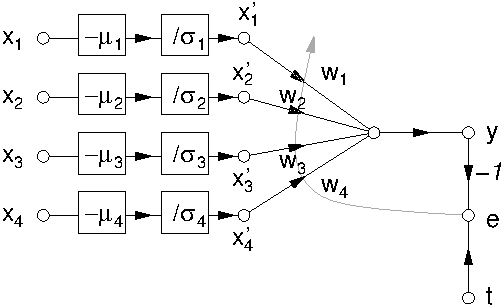
\includegraphics{lms-flow}
\end{center}
\caption{O diagrama de fluxo do discriminador LMS que será empregado na
discriminação elétron-jato.}
\label{fig:lms-flow}
\end{figure}

\subsection{Implementação do LMS na separação e\-lé\-tron-jato}
\label{sec:lms-ej}

Levando-se em consideração as 4 variáveis definidas pelo T2Calo, é possível
encontrar o plano quadri-dimensional que define um discriminador linear ótimo,
usando-se o algoritmo LMS, como descrito anteriormente. A separação em classes
de treinamento e teste, como apresentada na Seção~\ref{sec:eghypo}, será
re-aproveitada aqui, para que seja possível a comparação dos resultados nos
dois casos.

O sistema de treinamento e teste foi implementado em um ambiente de trabalho
C++, seguindo o paradigma da orientação à objetos (OO) \cite{stroustrup,
booch}. Este ambiente, que será re-utilizado em várias partes deste trabalho,
será discutido em detalhes na Seção~\ref{sec:framework}. A
Figura~\ref{fig:train-flow} contém um diagrama de fluxo com os diversos passos
do sistema de treinamento implementando. Inicialmente, os bancos de dados
usados para o treinamento e teste da rede são carregados. Os valores de média
e variância dos dados, levando-se em consideração a estatística de cada uma
das classes de dados, são extraídos do conjunto de treinamento e guardados
juntos aos pesos $\hat{w}(n)$, para que sejam aplicados durante o
treinamento\footnote{De fato, seria mais eficiente que os fatores de
normalização fossem aplicados previamente ao treinamento. No entanto, uma vez
que deseja-se re-aproveitar a base de código para rodar o discriminador em uma
etapa seguinte, é mais simples do ponto de vista da implementação que a
normalização seja aplicada como parte do passo de execução do
discriminador.}. Os pesos sinápticos são aleatoriamente inicializados (entre
$-1$ e $+1$). Valores-alvo para cada uma das classes são pré-fixados: $-1$
para elétrons e $+1$ para jatos. O processo de treinamento é então
disparado. Para cada época ou batelada de treinamento, um conjunto de elétrons
e jatos é escolhido aleatoriamente à partir dos bancos-de-dados
disponíveis. Os valores de erro são calculados e sua média é aplicada para a
correção dos pesos sinápticos, considerando a taxa de aprendizagem
$\alpha$. As melhores redes, tomando-se o valor do produto SP como referência,
são guardadas a cada passo de treinamento. 

\begin{figure}
\begin{center}
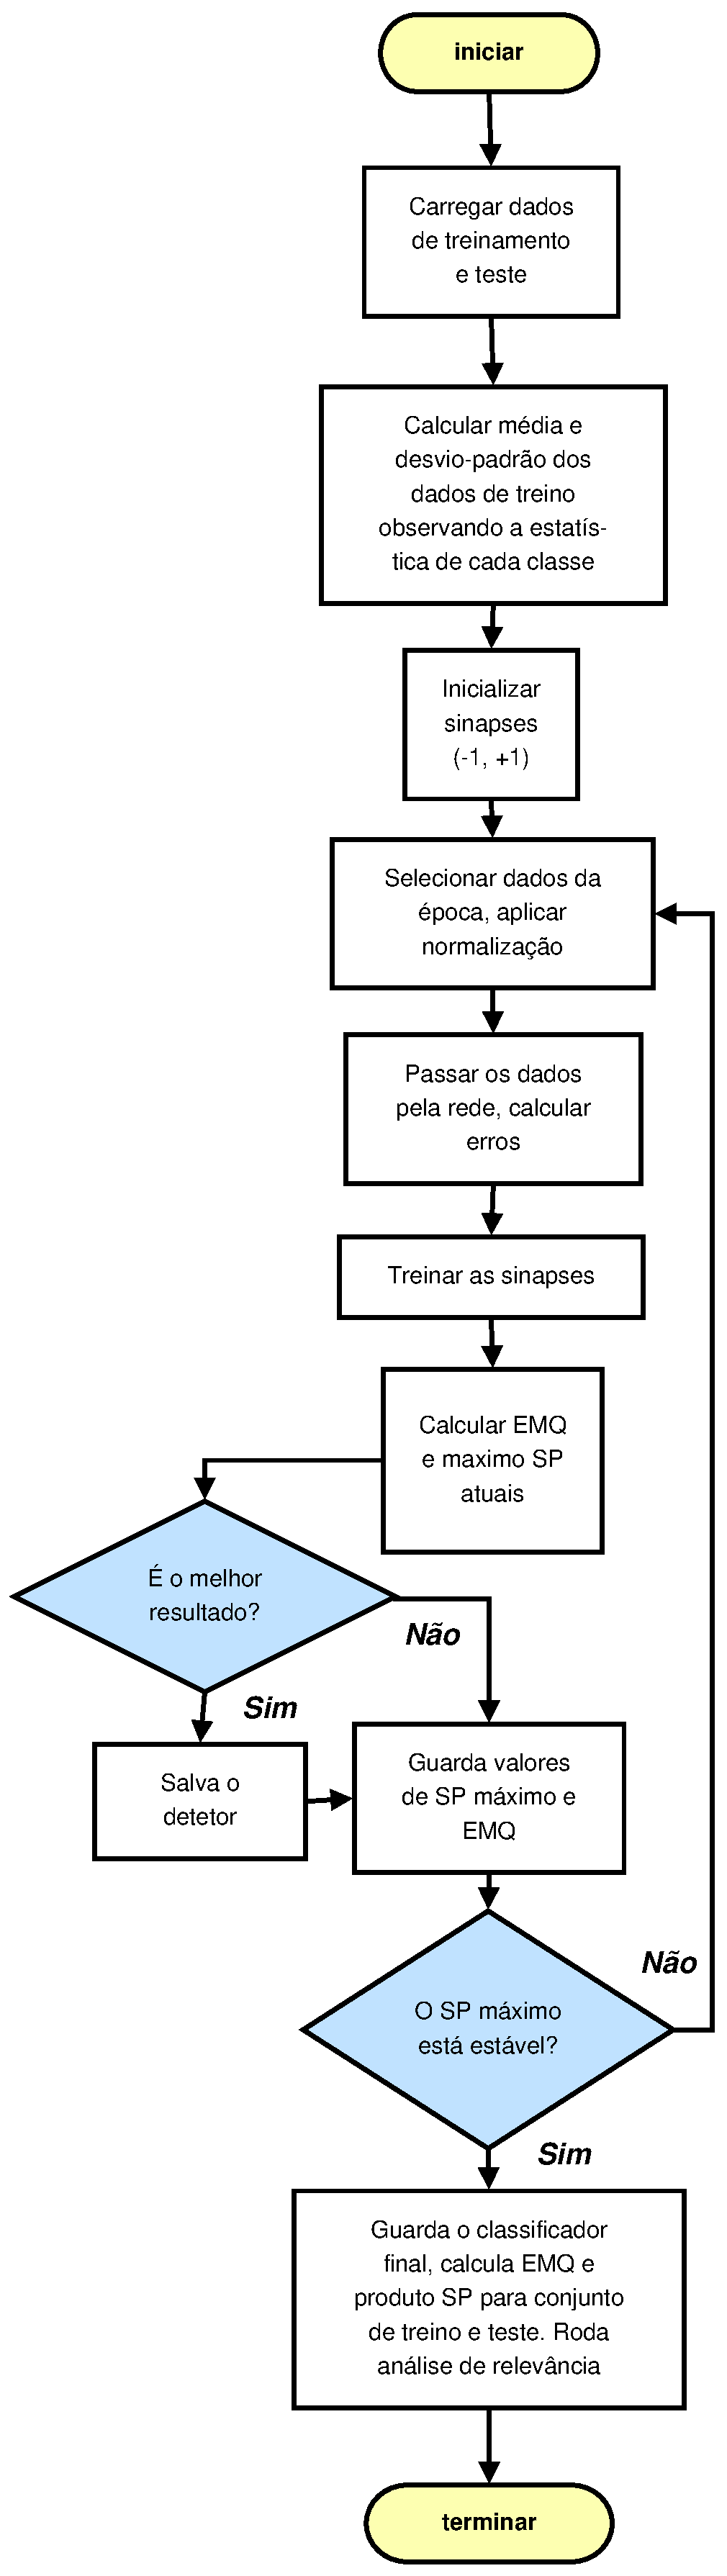
\includegraphics[scale=0.35]{train-flow}
\end{center}
\caption{O fluxo implementado para o treinamento do discriminador LMS.}
\label{fig:train-flow}
\end{figure}

Um sistema configurável é utilizado para detetar a estagnação do
treinamento. Este sistema baseia-se na observação do valor do produto SP para
o conjunto de teste. Quando este valor atinge um estado no qual as alterações
sinápticas não o modificam significativamente (levando-se em consideração uma
margem de erro configurável), e por um número de iterações, o treinamento é
automaticamente parado. O melhor discriminador até então é recarregado. Um
estudo dos valores de Erro Médio Quadrático (EMQ, do inglês \eng{Mean-square
error}, MSE) é feito para os conjuntos de treinamento e teste. O produto SP
máximo também é avaliado para os dois conjuntos de dados. Esta técnica tem o
objetivo de evitar um treinamento excessivo da rede (do inglês
\eng{overtraining}) fazendo com que ela se especialize em demasiado nestes
dados sem conseguir ter uma capacidade de discriminação generalizada. O valor
da variação do produto SP a partir do qual considera-se que o sistema esteja
estagnado dependerá do problema. Valores típicos estão na ordem de $10^{-3}$.

Para este trabalho, optou-se pela a não utilização de um conjunto de validação
do sistema de deteção. Este conjunto poderia ser utilizado para verificar a
operação do sistema após o treinamento. No entanto, a física disponível para o
estudo é limitada devido a natureza de geração de eventos. Para se realizar
uma análise baseada no LVL2, elétrons e jatos que passem a um corte do LVL1
devem ser simulados, uma vez que o LHC ainda não encontra-se operacional. 

A taxa de redução do LVL1 é bastante expressiva, atingindo uma redução de
aproximadamente 1000 vezes na taxa de contaminação de elétrons. Desta forma,
para produzir 1000 jatos que passariam a um corte do LVL1 é necessário que se
produza cerca de 1 milhão de eventos deste tipo. Cada simulação de um evento
pode durar muitos minutos, às vezes horas de processamento do poder de
computação disponível.

%Por outro lado, a física simulada é representativa do tipo de partículas
%que deseja-se analisar.

\subsection{Resultados da aplicação do LMS na separação e\-lé\-tron-jato}

Utilizando o sistema descrito anteriormente e a separação dos dados (em
classes de treinamento e teste) proposta no início do estudo, realizou-se um
conjunto de testes para a determinação de um discriminador linear ótimo
baseado nas quatro variáveis extraídas pelo T2Calo. Dois parâmetros foram
considerados neste exercício:

\begin{itemize}
\item O número de elementos na batelada ($N$);
\item O valor da taxa de treinamento ($\alpha$).
\end{itemize}

Embora seja possível assumir que o sistema convergirá em todas as condições,
valores muito grandes para a taxa de treinamento (ou pequenos para a
quantidade de eventos na batelada) poderão fazer o processo de convergência ao
mínimo parecer instável e disparar erros no sistema de parada automática do
treinamento. Desta forma, conduziu-se um conjunto de testes para a
determinação dos parâmetros de treinamento que acarretem em uma migração suave
ao erro mínimo do discriminador, no menor tempo possível. Os resultados podem
ser vistos nas Figuras~\ref{fig:lms-lr-analysis} e
\ref{fig:lms-esize-analysis}. Cada ponto nos gráficos representa a média sobre
dez treinamentos realizados à partir de um conjunto de pesos iniciais
sorteados (uniformemente) aleatoriamente no intervalo $[-1, +1]$. O desvio
padrão com relação a média define o tamanho da barra de erro. Durante o
experimento, limitou-se o número máximo de passos de treinamento em
$1.000$. Desta forma, pontos nas curvas próximos a este valor no eixo vertical
indicam provável que o treinamento foi interrompido bruscamente pelo programa.

\begin{figure}
\begin{center}
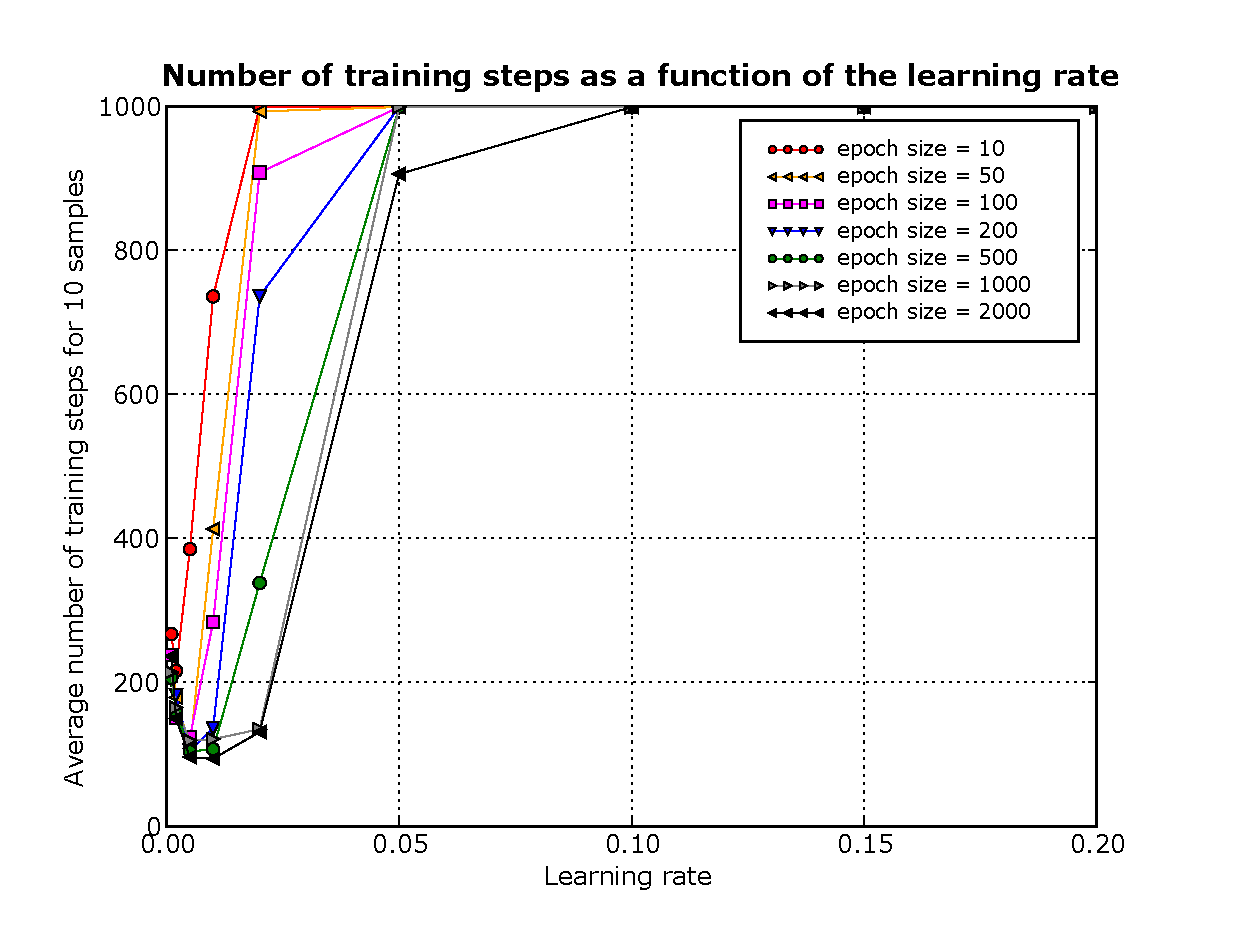
\includegraphics[scale=0.98]{lms/lms-lr-analysis}
\end{center}
\caption{Número de passos de treinamento médio para um detetor LMS baseado nas
4 características extraídas pelo T2Calo, em função da taxa de treinamento.}
\label{fig:lms-lr-analysis}
\end{figure}

\begin{figure}
\begin{center}
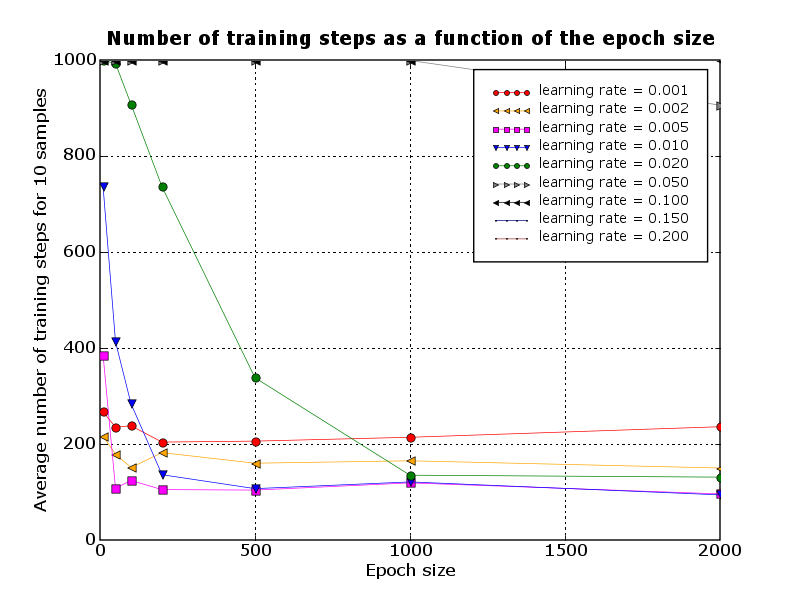
\includegraphics[scale=0.98]{lms/lms-esize-analysis}
\end{center}
\caption{Número de passos de treinamento médio para um detetor LMS baseado nas
4 características extraídas pelo T2Calo, em função do número de eventos por
época de treinamento.}
\label{fig:lms-esize-analysis}
\end{figure}

%\begin{table}
%\begin{center}
%\renewcommand{\baselinestretch}{1.0}
%{\tiny
%\begin{tabular}{|r|r|r|r|r|r|} \hline
%Taxa de treinamento ($\alpha$) & Época & Número de passos & Máximo SP (treino)
%& Máximo SP (teste) \\ \hline \hline 
%$0.0010$ & $10$ & $267\pm117.3$ & $1.5024\pm1.4\times 10^{-2}$ & $1.4975\pm1.7\times 10^{-2}$ \\ \hline
%$0.0010$ & $50$ & $235\pm50.8$ & $1.5045\pm2.1\times 10^{-2}$ & $1.5021\pm2.2\times 10^{-2}$ \\ \hline
%$0.0010$ & $100$ & $238\pm74.3$ & $1.5159\pm1.9\times 10^{-2}$ & $1.5114\pm1.6\times 10^{-2}$ \\ \hline
%$0.0010$ & $200$ & $204\pm62.0$ & $1.5193\pm1.6\times 10^{-2}$ & $1.5159\pm1.7\times 10^{-2}$ \\ \hline
%$0.0010$ & $500$ & $206\pm60.1$ & $1.5126\pm1.6\times 10^{-2}$ & $1.5078\pm1.7\times 10^{-2}$ \\ \hline
%$0.0010$ & $1000$ & $214\pm61.2$ & $1.5073\pm1.8\times 10^{-2}$ & $1.4996\pm1.7\times 10^{-2}$ \\ \hline
%$0.0010$ & $2000$ & $236\pm52.3$ & $1.5054\pm1.6\times 10^{-2}$ & $1.5009\pm1.4\times 10^{-2}$ \\ \hline
%$0.0020$ & $10$ & $216\pm42.7$ & $1.5122\pm1.0\times 10^{-2}$ & $1.5068\pm1.1\times 10^{-2}$ \\ \hline
%$0.0020$ & $50$ & $179\pm32.3$ & $1.5159\pm1.3\times 10^{-2}$ & $1.5129\pm1.1\times 10^{-2}$ \\ \hline
%$0.0020$ & $100$ & $151\pm29.4$ & $1.5111\pm1.4\times 10^{-2}$ & $1.5095\pm1.4\times 10^{-2}$ \\ \hline
%$0.0020$ & $200$ & $182\pm40.4$ & $1.5142\pm1.4\times 10^{-2}$ & $1.5088\pm1.6\times 10^{-2}$ \\ \hline
%$0.0020$ & $500$ & $160\pm42.0$ & $1.5077\pm2.0\times 10^{-2}$ & $1.5060\pm2.1\times 10^{-2}$ \\ \hline
%$0.0020$ & $1000$ & $165\pm34.2$ & $1.5089\pm1.7\times 10^{-2}$ & $1.5058\pm1.4\times 10^{-2}$ \\ \hline
%$0.0020$ & $2000$ & $150\pm35.8$ & $1.5080\pm1.3\times 10^{-2}$ & $1.5037\pm1.1\times 10^{-2}$ \\ \hline
%$0.0050$ & $10$ & $385\pm267.5$ & $1.5096\pm8.6\times 10^{-3}$ & $1.5053\pm7.6\times 10^{-3}$ \\ \hline
%$0.0050$ & $50$ & $108\pm33.8$ & $1.5150\pm1.2\times 10^{-2}$ & $1.5113\pm9.0\times 10^{-3}$ \\ \hline
%$0.0050$ & $100$ & $124\pm35.9$ & $1.5158\pm1.7\times 10^{-2}$ & $1.5096\pm1.5\times 10^{-2}$ \\ \hline
%$0.0050$ & $200$ & $105\pm23.2$ & $1.5191\pm1.4\times 10^{-2}$ & $1.5154\pm1.4\times 10^{-2}$ \\ \hline
%$0.0050$ & $500$ & $104\pm21.8$ & $1.5098\pm5.4\times 10^{-3}$ & $1.5066\pm6.3\times 10^{-3}$ \\ \hline
%$0.0050$ & $1000$ & $119\pm66.2$ & $1.5125\pm8.8\times 10^{-3}$ & $1.5100\pm8.0\times 10^{-3}$ \\ \hline
%$0.0050$ & $2000$ & $96\pm30.1$ & $1.5148\pm1.2\times 10^{-2}$ & $1.5123\pm1.2\times 10^{-2}$ \\ \hline
%$0.0100$ & $10$ & $736\pm422.9$ & $1.5153\pm6.9\times 10^{-3}$ & $1.5103\pm6.9\times 10^{-3}$ \\ \hline
%$0.0100$ & $50$ & $413\pm409.9$ & $1.5183\pm1.3\times 10^{-2}$ & $1.5140\pm1.1\times 10^{-2}$ \\ \hline
%$0.0100$ & $100$ & $284\pm228.8$ & $1.5116\pm1.0\times 10^{-2}$ & $1.5067\pm5.8\times 10^{-3}$ \\ \hline
%$0.0100$ & $200$ & $136\pm73.4$ & $1.5156\pm1.5\times 10^{-2}$ & $1.5124\pm1.5\times 10^{-2}$ \\ \hline
%$0.0100$ & $500$ & $107\pm36.0$ & $1.5145\pm1.2\times 10^{-2}$ & $1.5086\pm1.1\times 10^{-2}$ \\ \hline
%$0.0100$ & $1000$ & $121\pm46.1$ & $1.5122\pm1.5\times 10^{-2}$ & $1.5083\pm1.2\times 10^{-2}$ \\ \hline
%$0.0100$ & $2000$ & $94\pm35.7$ & $1.5136\pm1.1\times 10^{-2}$ & $1.5086\pm8.9\times 10^{-3}$ \\ \hline
%$0.0200$ & $10$ & $999\pm0.0$ & $1.5189\pm1.1\times 10^{-2}$ & $1.5130\pm1.1\times 10^{-2}$ \\ \hline
%$0.0200$ & $50$ & $993\pm17.4$ & $1.5152\pm1.4\times 10^{-2}$ & $1.5108\pm1.4\times 10^{-2}$ \\ \hline
%$0.0200$ & $100$ & $908\pm286.5$ & $1.5186\pm1.2\times 10^{-2}$ & $1.5156\pm1.2\times 10^{-2}$ \\ \hline
%$0.0200$ & $200$ & $736\pm423.5$ & $1.5195\pm1.4\times 10^{-2}$ & $1.5132\pm1.3\times 10^{-2}$ \\ \hline
%$0.0200$ & $500$ & $338\pm325.4$ & $1.5126\pm1.2\times 10^{-2}$ & $1.5097\pm1.2\times 10^{-2}$ \\ \hline
%$0.0200$ & $1000$ & $135\pm129.9$ & $1.5173\pm1.1\times 10^{-2}$ & $1.5113\pm1.0\times 10^{-2}$ \\ \hline
%$0.0200$ & $2000$ & $131\pm75.2$ & $1.5173\pm1.1\times 10^{-2}$ & $1.5128\pm1.2\times 10^{-2}$ \\ \hline
%$0.0500$ & $10$ & $999\pm0.0$ & $1.5263\pm1.4\times 10^{-2}$ & $1.5188\pm1.3\times 10^{-2}$ \\ \hline
%$0.0500$ & $50$ & $999\pm0.0$ & $1.5134\pm8.2\times 10^{-3}$ & $1.5117\pm9.3\times 10^{-3}$ \\ \hline
%$0.0500$ & $100$ & $999\pm0.0$ & $1.5239\pm1.2\times 10^{-2}$ & $1.5206\pm1.2\times 10^{-2}$ \\ \hline
%$0.0500$ & $200$ & $999\pm0.0$ & $1.5170\pm1.1\times 10^{-2}$ & $1.5113\pm1.1\times 10^{-2}$ \\ \hline
%$0.0500$ & $500$ & $999\pm0.0$ & $1.5109\pm9.6\times 10^{-3}$ & $1.5057\pm7.8\times 10^{-3}$ \\ \hline
%$0.0500$ & $1000$ & $999\pm0.0$ & $1.5154\pm1.1\times 10^{-2}$ & $1.5119\pm9.5\times 10^{-3}$ \\ \hline
%$0.0500$ & $2000$ & $906\pm220.9$ & $1.5122\pm1.2\times 10^{-2}$ & $1.5087\pm1.4\times 10^{-2}$ \\ \hline
%$0.1000$ & $10$ & $999\pm0.0$ & $1.5332\pm5.5\times 10^{-3}$ & $1.5246\pm8.4\times 10^{-3}$ \\ \hline
%$0.1000$ & $50$ & $999\pm0.0$ & $1.5256\pm1.4\times 10^{-2}$ & $1.5177\pm1.2\times 10^{-2}$ \\ \hline
%$0.1000$ & $100$ & $999\pm0.0$ & $1.5229\pm7.5\times 10^{-3}$ & $1.5143\pm4.9\times 10^{-3}$ \\ \hline
%$0.1000$ & $200$ & $999\pm0.0$ & $1.5174\pm1.3\times 10^{-2}$ & $1.5101\pm1.1\times 10^{-2}$ \\ \hline
%$0.1000$ & $500$ & $999\pm0.0$ & $1.5072\pm1.0\times 10^{-2}$ & $1.5023\pm7.2\times 10^{-3}$ \\ \hline
%$0.1000$ & $1000$ & $999\pm0.0$ & $1.5188\pm1.2\times 10^{-2}$ & $1.5149\pm1.2\times 10^{-2}$ \\ \hline
%$0.1000$ & $2000$ & $999\pm0.0$ & $1.5209\pm8.9\times 10^{-3}$ & $1.5167\pm6.6\times 10^{-3}$ \\ \hline
%$0.1500$ & $10$ & $999\pm0.0$ & $1.5385\pm8.0\times 10^{-3}$ & $1.5271\pm4.4\times 10^{-3}$ \\ \hline
%$0.1500$ & $50$ & $999\pm0.0$ & $1.5251\pm9.5\times 10^{-3}$ & $1.5178\pm1.0\times 10^{-2}$ \\ \hline
%$0.1500$ & $100$ & $999\pm0.0$ & $1.5203\pm1.3\times 10^{-2}$ & $1.5154\pm1.1\times 10^{-2}$ \\ \hline
%$0.1500$ & $200$ & $999\pm0.0$ & $1.5178\pm1.1\times 10^{-2}$ & $1.5112\pm9.7\times 10^{-3}$ \\ \hline
%$0.1500$ & $500$ & $999\pm0.0$ & $1.5180\pm1.1\times 10^{-2}$ & $1.5125\pm9.6\times 10^{-3}$ \\ \hline
%$0.1500$ & $1000$ & $999\pm0.0$ & $1.5150\pm8.5\times 10^{-3}$ & $1.5086\pm8.6\times 10^{-3}$ \\ \hline
%$0.1500$ & $2000$ & $999\pm0.0$ & $1.5138\pm1.1\times 10^{-2}$ & $1.5076\pm1.0\times 10^{-2}$ \\ \hline
%$0.2000$ & $10$ & $999\pm0.0$ & $1.5409\pm5.5\times 10^{-3}$ & $1.5329\pm4.8\times 10^{-3}$ \\ \hline
%$0.2000$ & $50$ & $999\pm0.0$ & $1.5242\pm9.9\times 10^{-3}$ & $1.5182\pm6.7\times 10^{-3}$ \\ \hline
%$0.2000$ & $100$ & $999\pm0.0$ & $1.5256\pm9.1\times 10^{-3}$ & $1.5149\pm7.1\times 10^{-3}$ \\ \hline
%$0.2000$ & $200$ & $999\pm0.0$ & $1.5214\pm9.3\times 10^{-3}$ & $1.5143\pm7.5\times 10^{-3}$ \\ \hline
%$0.2000$ & $500$ & $999\pm0.0$ & $1.5201\pm8.3\times 10^{-3}$ & $1.5140\pm6.7\times 10^{-3}$ \\ \hline
%$0.2000$ & $1000$ & $999\pm0.0$ & $1.5248\pm1.3\times 10^{-2}$ & $1.5174\pm1.2\times 10^{-2}$ \\ \hline
%$0.2000$ & $2000$ & $999\pm0.0$ & $1.5133\pm1.1\times 10^{-2}$ & $1.5080\pm1.1\times 10^{-2}$ \\ \hline
%\end{tabular}
%}
%\renewcommand{\baselinestretch}{1.5}
%\end{center}
%\caption{Média de passos de treinamento e máximos de produto SP em função da
%taxa de aprendizagem e tamanho da época para um classificador LMS elétron/jato
%baseado nas saídas do T2Calo.}
%\label{tab:lms-scan}
%\end{table}

Uma análise visual nestes gráficos indica que valores de taxa de treinamento
que minimizem o tempo de treinamento estão na faixa onde $\alpha < 0.02$,
enquanto que para o tamanho da época, em $N \geq 500$. Escolhe-se $N = 500$ e
$\alpha = 0.01$. Desta forma, depois de cerca de 10 passos, $5000$ eventos
terão sido apresentados a rede. Com 40 ou 50 passos, o sistema de treinamento
terá, possivelmente, apresentado todos os dados de treinamento ao menos uma
vez.\footnote{O sorteio dos eventos de uma batelada é feito de forma aleatória
seguindo uma distribuição uniforme e não há garantias que todos os eventos
sejam utilizados ao longo do treinamento, embora seja estatisticamente
provável que isto aconteça após um certo número de épocas. Esta probabilidade
aumenta com o número de eventos por época e com o número de épocas de
treinamento a qual a rede foi submetida.}.

A Figura~\ref{fig:lms-mse-evo} mostra a evolução do EMQ para uma das 10 redes
com $N = 500$ e $\eta = 0.01$, tanto para o conjunto de treinamento (no alto)
quanto para o conjunto de teste (embaixo). A Figura~\ref{fig:lms-sp-evo}
mostra um gráfico equivalente, mas para o produto SP, ao invés do EMQ. Como é
possível verificar, o sistema converge depois de pouco menos que 100 passos de
treinamento. A evolução do produto SP aumenta rapidamente no início do
treinamento, por cerca de 20 passos e depois permanecendo constante, em
aproximadamente 1,5 para o restante do treinamento. O mesmo não ocorre para o
EMQ que ainda continuará a diminuir, significativamente, por mais 60 a 80
passos antes da deteção automática da parada. Este comportamento indica que,
apesar do sistema conseguir aproximar melhor os alvos na saída, sua capacidade
discriminatória mantém-se praticamente inalterada após os 20 passos
iniciais. O perfil de evolução do produto SP e minimização do EMQ é seguido
pelo conjunto de teste, de forma bastante semelhante, indicando que a
estatística disponível no conjunto treino é representativa dos dados no
conjunto de teste.

%É interessante notar que após 20 passos de treinamento, $10000$
%elementos terão sido utilizados no treinamento da rede. Este valor é menor que
%o tamanho do conjunto de treinamento, com cerca de $15000$ elementos,
%indicando que o conjunto de dados, para a análise linear, ...

\begin{figure}
\begin{center}
\includegraphics[scale=0.98]{lms/mse-evolution}
\end{center}
\caption{Evolução dos valores do E.M.Q. ao longo do treinamento do detetor
LMS, para o conjunto de treinamento (topo) e de teste (embaixo). A taxa de
treinamento para este sistema é $0,01$ equanto que o tamanho da época
escolhido é $500$.}
\label{fig:lms-mse-evo}
\end{figure}

\begin{figure}
\begin{center}
\includegraphics[scale=0.98]{lms/sp-evolution}
\end{center}
\caption{Evolução dos valores do produto SP ao longo do treinamento do detetor
LMS, para o conjunto de treinamento (topo) e de teste (embaixo). A taxa de
treinamento para este sistema é $0,01$ equanto que o tamanho da época
escolhido é $500$.}
\label{fig:lms-sp-evo}
\end{figure}

A Figura~\ref{fig:lms-test-output} mostra os histogramas da saída da rede para
elétrons (alto) e jatos (embaixo), considerando-se o conjunto de teste. O
ponto ótimo de corte, determinado para que se maximize o produto SP da rede
para o conjunto de treinamento para este sistema é $-0,0473$. Nestas
condições, o máximo produto SP para o conjunto de teste é 1,51, definido no
ponto da curva R.O.C. (veja Figura~\ref{fig:lms-test-roc}) onde a eficiência
para a deteção de elétrons é 91,64\% enquanto que a eficiência para a deteção
de jatos é de 90,35\%. A Figura~\ref{fig:lms-vs-egamma-roc} mostra uma
comparativo entre o resultado da otimização proposta atualmente no experimento
ATLAS contra os resultados obtidos para este classificador. Através desta
figura é possível observar que o discriminador LMS tangencia a parte exterior
dos pontos da otimização proposta atualmente no experimento. O resultado
obtido com o algoritmo LMS, ao invés do longo processo de otimização proposto
originalmente, é atingido depois de apenas 1 minuto e 30 segundos de
treinamento em um computador dotado de um processador AMD 64 com \eng{clock}
de 2~GHz e 1~Gb de memória RAM. Ademais, tal sistema apresenta uma capacidade
discriminatória praticamente ótima após apenas 20 passos de treinamentos, isto
é, $\approx 25$ segundos na máquina citada.

\begin{figure}
\begin{center}
\includegraphics[scale=0.98]{lms/test-output}
\end{center}
\caption{Saída do detetor LMS em estudo para o conjunto de treino.}
\label{fig:lms-test-output}
\end{figure}

\begin{figure}
\begin{center}
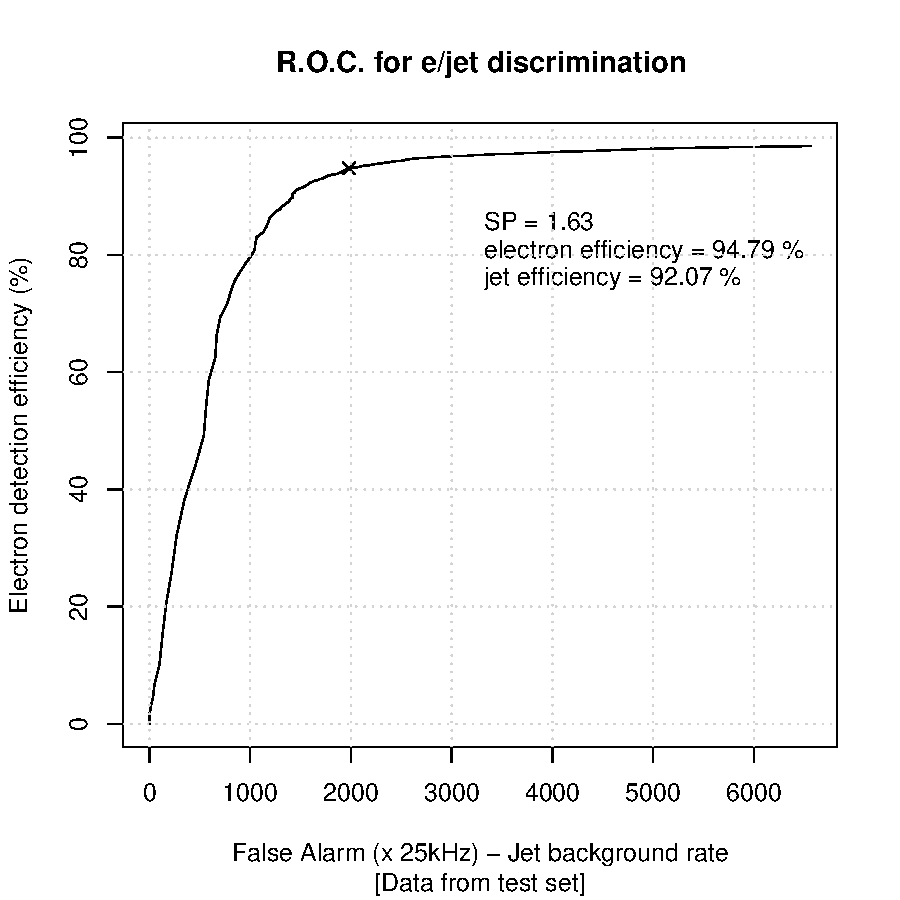
\includegraphics[scale=0.98]{lms/test-roc}
\end{center}
\caption{Curva R.O.C. para um detetor elétron/jato baseado no detetor LMS em
estudo.}
\label{fig:lms-test-roc}
\end{figure}

\begin{figure}
\begin{center}
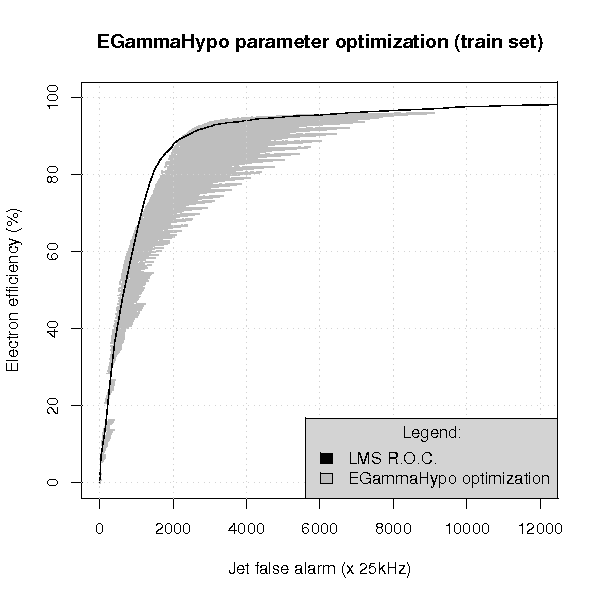
\includegraphics[scale=0.98]{lms/lms-vs-egamma-roc}
\end{center}
\caption{R.O.Cs comparativas entre a otimização atual para o EGammaHypo e um
detetor baseado no LMS.}
\label{fig:lms-vs-egamma-roc}
\end{figure}

As Figuras~\ref{fig:lms-test-sp-eta}, \ref{fig:lms-test-sp-phi} e
\ref{fig:lms-test-sp-emet} mostram, respectivamente, o valor do produto SP segundo
a distribuição dos dados em $\eta$, $\phi$ e $\etem$. O número anexo ao topo
de cada barra indica a quantidade de cada canal e é útil para que se considere
a relevância de um valor parcial no desempenho do discriminador. Nota-se que
na distribuição por $\eta$, há uma clara perda de eficiência na região
$|\eta| \approx 1,5$. Esta notável queda no desempenho do classificador é
devido a um espaço sem elementos de deteção nesta área (também conhecido como
\eng{gap} ou \eng{crack} dos calorímetros), por onde passam os cabos de
leitura e manutenção dos detetores internos. A eficiência é recuperada logo
após esta região. O gráfico de barras para a distribuição $\phi$ mostra-se
praticamente uniforme, indicando que o sistema funciona sem tendências para
todos os valores desta variável. Este resultado é esperado, já que o detetor é
simétrico neste eixo. A análise por $\etem$ demonstra uma predominante
qualidade de deteção para valores mais baixos de energia que valores mais
altos. Deve-se levar em conta que, embora a eficiência de deteção de elétrons
ainda seja máxima nesta última região, como mostra a
Figura~\ref{fig:lms-test-efficiency-emet}, o falso alarme na deteção de jatos
também apresenta-se máximo. Uma vez que o produto SP é uma figura de mérito da
eficiência agregada de ambas as classes de eventos do discriminador, ela
quantificar-se-á em zero nesta região. Este resultado está associado a baixa
estatística de dados disponível na região.

\begin{figure}
\begin{center}
\includegraphics[scale=0.98]{lms/test-sp-eta}
\end{center}
\caption{Análise do produto SP do detetor LMS, para os dados do conjunto de
teste ao longo de $\eta$.}
\label{fig:lms-test-sp-eta}
\end{figure}

\begin{figure}
\begin{center}
\includegraphics[scale=0.98]{lms/test-sp-phi}
\end{center}
\caption{Análise do produto SP do detetor LMS, para os dados do conjunto de
teste ao longo de $\phi$.} 
\label{fig:lms-test-sp-phi}
\end{figure}

\begin{figure}
\begin{center}
\includegraphics[scale=0.98]{lms/test-sp-emet}
\end{center}
\caption{Análise do produto SP do detetor LMS, para os dados do conjunto de
teste por $\etem$.} 
\label{fig:lms-test-sp-emet}
\end{figure}

\begin{figure}
\begin{center}
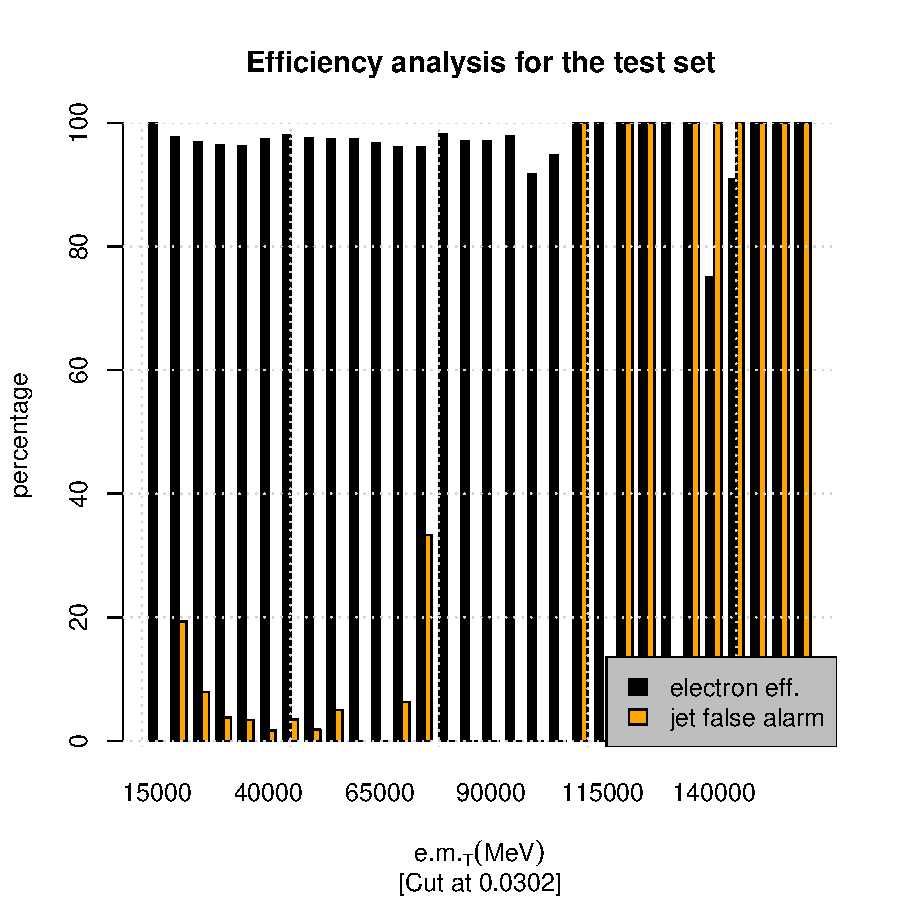
\includegraphics[scale=0.98]{lms/test-efficiency-emet}
\end{center}
\caption{Análise da eficiência de deteção de elétrons e falso alarme em jatos
para o detetor LMS, utilizando os dados do conjunto de teste, por $\etem$.}
\label{fig:lms-test-efficiency-emet}
\end{figure}

A Figura~\ref{fig:lms-vs-egamma} mostra um comparativo entre as duas técnicas
de deteção, por energia transversa na seção e.m.. Distingue-se que os dois
sistemas possuem respostas bastante próximas. Na primeira (mais à esquerda)
faixa de energia considerada, o EGammaHypo possui uma resposta melhor enquanto
que com o aumento da energia transversa o LMS apresenta-se mais eficiente, e
segue este padrão para quase todas as faixas consideradas, principalmente onde
há maior concentração de eventos de teste, como é possível determinar à partir
da Figura~\ref{fig:lms-test-sp-emet}.

\begin{figure}
\begin{center}
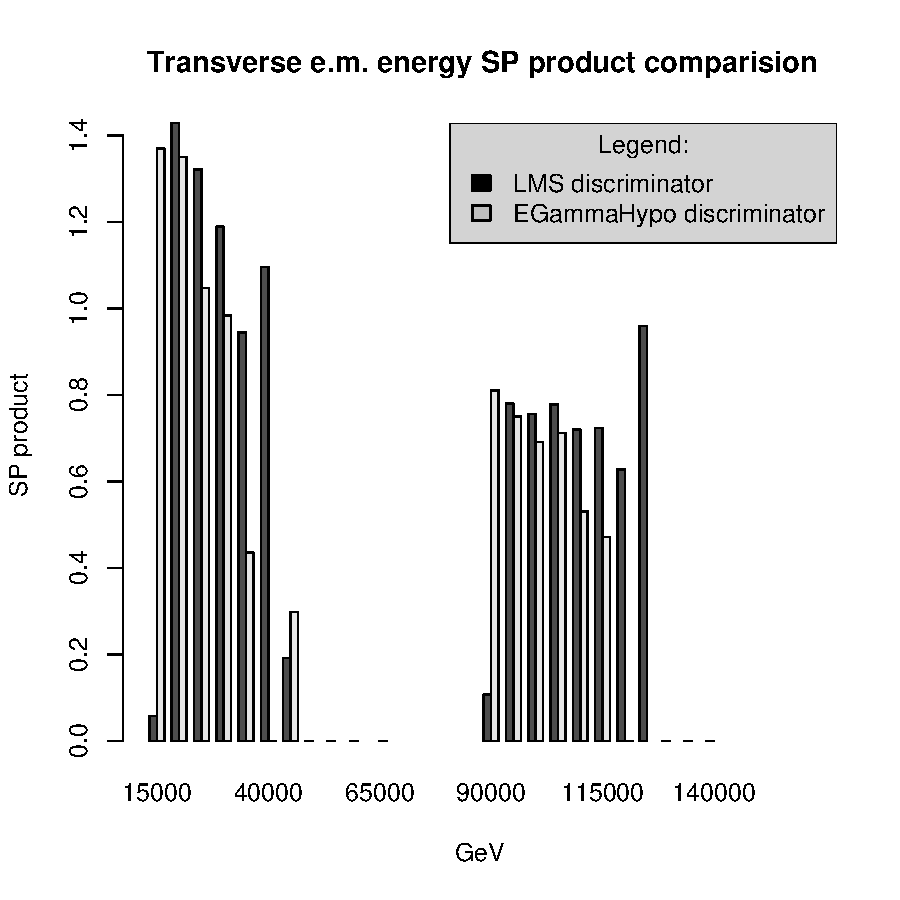
\includegraphics[scale=0.98]{lms/lms-vs-egamma}
\end{center}
\caption{Comparação do produto SP para um classificador baseado no LMS e o
EGammaHypo por energia transversa na seção e.m..}
\label{fig:lms-vs-egamma}
\end{figure}

\subsection{Relevância das características do T2Calo}

A técnica da análise de relevância \cite{relevance} tem por objetivo medir a
importância de cada uma das variáveis de entrada para um classificador. Nesta
técnica, suprime-se a contribuição da variável à composição da saída
substituindo-se seu valor, a cada evento, por sua média, para todos os eventos
disponíveis na entrada do sistema de discriminação. Observando-se a variação
da saída, é possível estimar a contribuição daquela variável ao processo
discriminatório. A estimativa de relevância da i-ésima componente de entrada
pode, então ser calculada pela fórmula:

\begin{equation}
R_i = \frac{1}{N} \text{ } \overset{N}{\underset{j=1}{\sum}} \text{ }
[\text{saída}(\overrightarrow{x_j}) -
\text{saída}(\overrightarrow{x_j}\mid_{x_{j,i} = \overline{x}_i})]^2 
\label{eq:relevance-mse}
\end{equation}

Em outras palavras, é possível definir a relevância da variável $x_i$, $R_i$,
como o EMQ da saída de um discriminador comparada a mesma saída quando faz-se
a variável assumir o valor de sua média. Nessa equação, $N$ representa o
número total de eventos (padrões) disponíveis para o classificador. A
Figura~\ref{fig:relevance-mse} mostra os valores de relevância para cada uma
das variáveis do classificador em análise. Esta figura mostra, mais uma vez,
que o conjunto de treino permite generalizar o comportamento do discriminador,
apresentando valores de relevância, para cada uma de suas variáveis, bastante
próximos daqueles valores calculados para o conjunto de teste. Esta figura
também mostra que a variável $\rcore$ é de extrema importância na determinação
da saída do detetor. Quando substituímo-la por sua média, o erro na saída
aumenta de mais de 3 pontos enquanto que para as demais variáveis, o impacto é
nitidamente menor. Esta figura também indica que a ordem de separação proposta
pelo EGammaHypo está em acordo com o processo de filtragem definido
automaticamente pelo LMS, levando-se em consideração a ordem onde os cortes
são aplicados por aquele algoritmo e a importância das variáveis nesse
processo de classificação. A importância destas variáveis ao sistema LMS
poderia ser utilizada para simplificá-lo. Por exemplo, seria possível
``podar'' a variável menos relevante e re-treinar o sistema para obter um
classificador mais rápido.

\begin{figure}
\begin{center}
\includegraphics[scale=0.98]{lms/relevance-mse}
\end{center}
\caption{Os valores de relevância para os conjunto de treino (cinza claro) e
teste (em cinza escuro), para as 4 variáveis do T2Calo e considerando-se o
classificador LMS em estudo.}
\label{fig:relevance-mse}
\end{figure}

Por outro lado, como foi visto nas análises de evolução do EMQ
(Figura~\ref{fig:lms-mse-evo}) e do produto SP (Figura~\ref{fig:lms-sp-evo}),
a capacidade discriminatória da rede reage de forma correlacionada, mas
\textbf{não necessariamente} idêntica ao processo de mapeamento da entrada
na saída proposto pelo LMS. Observa-se que, apesar de notarmos uma contínua
migração ao mínimo EMQ durante cerca de 100 passos de treinamento, após cerca
de apenas 20 passos, a capacidade discriminatória do sistema já atinge seu
máximo e ali permanece até o final do treinamento. Este comportamento indica
que exista uma diferença não-negligível entre estes dois parâmetros. Desta
forma, propõe-se uma variação do cálculo da relevância, mas agora baseando-se
no impacto da substituição do valor da variável pela sua média à capacidade
discriminatória da rede, agora representada pela variação do produto SP, da
seguinte forma:

\begin{equation}
R_{d_i} = \max(\text{SP}_{\text{original}}) - \max(\text{SP}(\overrightarrow{x_j}\mid_{x_{j,i} = \overline{x}_i}))
\label{eq:relevance-sp}
\end{equation}

Neste caso define-se a relevância $R_{d_i}$ da variável $i$ como a diferença
no produto SP máximo causado pela substituição desta variável pela sua
média. De fato, espera-se que a maior parte dos valores de relevância sejam
positivos, indicando uma degradação do desempenho do classificador seguindo a
neutralização de uma variável. Seria possível que se encontrasee valores de
relevância negativos, o que indicaria que uma variável está, na verdade,
atrapalhando o processo de classificação ao invés de melhorá-lo. A
Figura~\ref{fig:relevance-sp} mostra os valores de $R_d$ para o classificador
LMS em estudo. Como é possível ver nesta figura, o quadro é marginalmente
diferente daquele mostrado pela Figura~\ref{fig:relevance-mse}. A variável
mais importante para o processo discriminatório é ainda $\rcore$, seguindo-se
de $\eratio$ e $\ethad$. A variável $\etem$ é a menos relevante para o
processo de classificação de elétrons e jatos, o que já era esperado
observando-se as tendências com o EGammaHypo. Como é possível definir à partir
deste gráfico, seria preferencial uma poda da variável $\etem$ que da variável
$\ethad$, como sugeriria a Figura~\ref{fig:relevance-mse}. No mais, as duas
figuras são bastante compatíveis e indicam uma tendência importante: a
minimização do EMQ também maximizará o produto SP. Esta figura também
indicaria que a ordem na qual o EGammaHypo considera as variáveis de corte
(i.e. $\rcore \rightarrow
\eratio \rightarrow \etem \rightarrow \ethad$) seja não-ótima para o conjunto
de dados sendo analisado, mesmo que marginalmente. Observa-se que seria mais
interessante que o corte em $\etem$ fosse realizado por último ao invés do
corte em $\ethad$, pois desta forma o processo discriminatório seria mais
rápido.

\begin{figure}
\begin{center}
\includegraphics[scale=0.98]{lms/relevance-sp}
\end{center}
\caption{Os valores de relevância de discriminação para os conjunto de treino
(cinza claro) e teste (em cinza escuro), para as 4 variáveis do T2Calo e
considerando-se o classificador LMS em estudo.}
\label{fig:relevance-sp}
\end{figure}

\section{Métodos neurais de discriminação}
\label{sec:neural}

Redes neurais artificiais (RNA) vêm sendo atualmente utilizadas com sucesso em
problemas de otimização, controle e reconhecimento de padrões
\cite{haykin}. RNA's são modelos matemáticos inspirados no conhecimento
limitado que temos do cérebro animal. Neste contexto, entende-se que uma rede
neural pode aprender através do contato com os elementos de interesse de um
determinado espaço de entrada e que este conhecimento é armazenado através das
conexões sinápticas que conectam os elementos processadores (neurônios) da
rede. Dentre as características de uma RNA podemos destacar:

\begin{description}
\item[Robustez] Em ambientes extremamente \emph{agressivos} (sujeitos a falhas
e a radioatividade), como é o caso da operação do ATLAS, RNA's podem manter um
excelente desempenho, mesmo quando parte dos dados (canais de aquisição) de
entrada são perdidos;

\item[Generalização] RNA's podem extrair a informação relevante escondida sob
uma grande quantidade de ruído;

\item[Deteção de novos fenômenos] RNA's podem detetar a ocorrência de novos
objetos de forma bastante eficaz. Isto é \underline{extremamente} importante
em ambientes que podem revelar resultados inesperados (nova física);

\item[Simples implementação] RNA's podem ser facilmente descritas em
linguagens de programação convencionais, atingindo desempenhos satisfatórios
para um grande conjunto de aplicações em tempo real.
\end{description}

A utilização de RNA's em experimentos em Física de Altas Energias também vem
se popularizando ao longo das últimas década, principalmente na área de
calorimetria, tanto especificamente em sistemas de filtragem \cite{badgett92,
koehne96} quanto para análise pós-reconstrução \cite{altherr90}. Isto se deve
principalmente ao fato que RNA's consigam definir uma superfície de separação
não-linear no espaço de dados sendo considerado, normalmente atingindo
resultados bastante acurados na determinação do \eng{background} e ainda
retendo um desempenho satisfatório quando comparadas às técnicas de deteção
por cortes como as discutidas anteriormente (veja a
Seção~\ref{sec:def-eghypo}).

\subsection{Introdução ao processamento neural}

A Figura~\ref{fig:neuron} contém uma modelagem de um neurônio
genérico. Analogamente ao sistema LMS descrito na Seção~\ref{sec:lms}, os
elementos processadores de uma rede neural, chamados neurônios ou percéptrons,
são ativados por um conjunto de entradas $\overrightarrow{x}$, somadas de
acordo com um sistema linear de ponderação $\overrightarrow{w}$. O diferencial
entre o sistema linear proposto anteriormente e um neurônio está na função de
ativação que conduz o campo induzido $v_p =
\overrightarrow{x}*\overrightarrow{w}_{p}^{T}$ à saída. Enquanto que
no caso do LMS utiliza-se a função identidade, i.e., $y_p = v_p$, no caso de
percéptrons, faz-se uso de uma função não-linear, como por exemplo a função
tangente hiperbólica:

\begin{figure}
\begin{center}
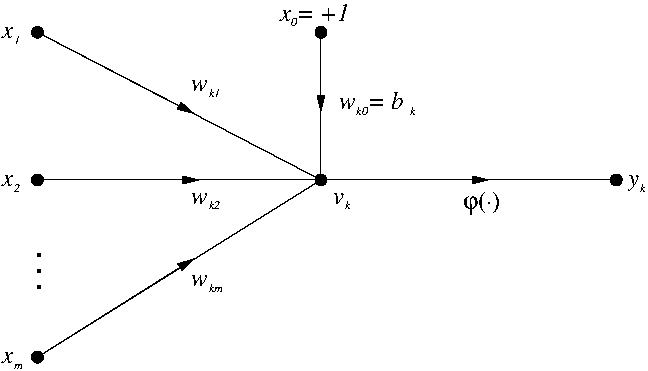
\includegraphics{neuron}
\end{center}
\caption{Grafo de fluxo de sinal de um neurônio artificial.}
\label{fig:neuron}
\end{figure}

\begin{equation}
tanh(v) = \frac{e^v - e^{-v}}{e^v + e^{-v}} = \frac{e^{2v} - 1}{e^{2v} + 1}
\label{eq:tanh}
\end{equation}

Ou a função logística (simplificada):

\begin{equation}
P(v) = \frac{1}{1 + e^{-v}}
\label{eq:logf}
\end{equation}

A razão da escolha de uma função não-linear para a ativação de um campo
induzido pode ser qualificado à partir da seguinte constatação: se sistema a
que se deseja classificar aprensenta um comportamento gaussiano, para ambas as
classes, i.e., os momentos de ordem superior a $2$ para ambas as classes são
todos iguais a zero, o classificador ótimo (bayesiano) resume-se um sistema
linear \cite{haykin}. Naturalmente nota-se que seja sempre possível
\textit{aproximar} ou modelar um sistema não-gaussiano em um desta espécie,
tendo por conseqüência os erros relativos a esta aproximação. De fato, foi o
que foi realizado na Seção~\ref{sec:lms-ej}, quando escolhou-se utilizar um
classificador linear para separar as quatro variáveis definidas pelo T2Calo.

Se o sistema que se deseja resolver apresenta um comportamento não-gaussiano,
o classificador ótimo não pode ser representando por um classificador
linear. Neste caso, utiliza-se uma função de ativação não-linear para que se
aproxime, de alguma forma, o comportamento não-linear do sistema de interesse.
As funções nas Equações~(\ref{eq:tanh}) e (\ref{eq:logf}) são normalmente
utilizadas por apresentarem amplitude limitada e possuírem derivada
trivialmente calculável. A razão de procurar-se funções com derivadas simples
(e suaves) ficará mais clara adiante, quando se definir o algoritmo de
treinamento. A amplitude limitada pode rapidamente ser verificada como uma
característica de interesse observando-se que o treinamento de um sistema que
trabalha por aprendizado seja muitas vezes executado com a retro-alimentação
de erros. Neste caso, para evitar oscilações e pontos de ressonância, um
sistema cuja a saída seja limitada apresenta natural vantagem se comparado a
outro análogo \cite{haykin}.

Este estudo está focado na utilização de RNA's utilizando percéptrons em
múltiplas camadas (do inglês \eng{Multi-layer perceptrons} ou MLP),
completamente conectadas, sem realimentação e com treinamento baseado na
retropropagação de erros. Introduziremos o processo de treinamento destes
sistemas à seguir.

\subsection{Treinamento por retro-propagação de erros}

Para sistemas com apenas uma camada neural, observa-se que, ao buscar-se o
ponto de mínimo da superfície de erro (quadrático), naturalmente otimiza-se o
conjunto de pesos de tal forma que o sistema consiga mapear a entrada nos
alvos de saída. A única restrição do método é que a função de ativação do
campo induzido do neurônio $\varphi(\cdot)$ seja diferenciável.
\cite{rosenblatt}. O problema do treinamento de uma rede MLP é um pouco mais
complexo. Um grafo de fluxo de uma rede MLP completamente conectada pode ser
visto na Figura~\ref{fig:simple-mlp}. Neste caso considera-se que a rede
possui apenas uma camada escondida e apenas um neurônio de saída pois se
identifica intimamente com os casos de uso que abordaremos. Ainda sim, seria
possível considerar casos com um número maior de neurônios de saída ou com
mais camadas escondidas generalizando os casos exemplificados aqui.

\begin{figure}
\begin{center}
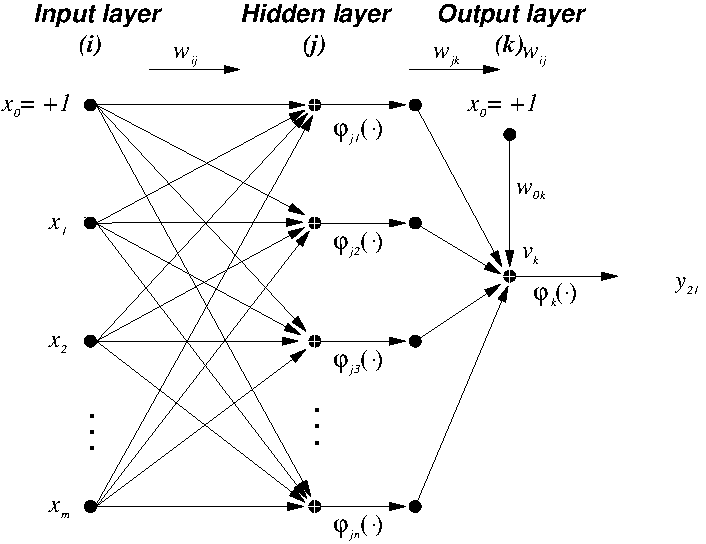
\includegraphics{simple-mlp}
\end{center}
\caption{Modelagem de uma rede MLP, totalmente conectada e sem
retro-propagação de sinal.}
\label{fig:simple-mlp}
\end{figure}

Para o sistema em questão, o mecanismo de treinamento para o neurônio de saída
é idêntico ao treinamento de um percéptron simples, e pode ser facilmente
definido da seguinte forma:

\begin{align}
\text{Se define-se o erro como } \mathcal{E}(n) &= \frac{1}{2}e_{k}^{2}(n)
\label{eq:error-def} \\
\text{e considerando-se que } \frac{\partial\mathcal{E}(n)}{\partial
w_{jk}(n)} &= \frac{\partial\mathcal{E}(n)}{\partial e_k(n)} \frac{\partial
e_k(n)}{\partial y_k(n)} \frac{\partial y_k(n)}{\partial v_k(n)}
\frac{\partial v_k(n)}{\partial w_{jk}(n)} \label{eq:partials} \\
\text{ou seja, } \frac{\partial\mathcal{E}(n)}{\partial
w_{jk}(n)} &= e_k(n)(-1)\varphi_{k}'(v_{k}(n))y_{k}(n)
\label{eq:partials-solution} \\
\text{e, resumindo, } \Delta w_{jk}(n) &=
-\eta\frac{\partial\mathcal{E}(n)}{\partial w_{jk}(n)} = \eta
e_{k}(n)\varphi_{k}'(v_{k}(n))y_{k}(n)
\end{align}

Normalmente, define-se:

\begin{align}
\text{Gradiente local: } \delta_k(n) &= - e_k(n)\varphi_{k}'(v_k(n)) \\
\text{e desta forma } \Delta w_{jk}(n) &= \eta\delta_k(n)y_{k}(n)
\label{eq:neural-train}
\end{align}

Este sistema de equações segue o princípio definido anteriormente para o LMS,
mas sem assumir nada sobre a função de ativação $\varphi(\cdot)$. Nota-se que
para uma função de ativação onde $y_k(n) = v_k(n)$, recai-se no algoritmo de
treinamento do LMS: $\Delta w_{jk}(n) = \eta e_{j}(n)y_{j}(n)$. Desta forma, é
possível considerar o LMS como um caso especial de uma rede neural com apenas
uma camada e cuja a função de ativação é a função identidade. Nestas equações,
$n$ representa a época ou batelada de treinamento.

O segundo caso de interesse acontece quando o neurônio $j$ está localizado em
uma camada oculta da rede. Neste caso, não existe uma resposta desejada (alvo)
específica para aquele neurônio. Desta forma, tentar-se-á definir o sinal de
erro de um neurônio escondido recursivamente, através da retro-propagação do
erro na saída final da rede em direção ao neurônio desejado. Iniciamos,
intuitivamente, com a definição do gradiente local do neurônio escondido $j$:

\begin{equation}
\delta_j(n) = -\frac{\partial\mathcal{E}(n)}{\partial
v_j(n)} = -\frac{\partial\mathcal{E}(n)}{\partial
y_j(n)}\frac{\partial y_j(n)}{\partial v_j(n)} =
-\frac{\partial\mathcal{E}(n)}{\partial y_j(n)}\varphi_{j}'(v_j(n))
\end{equation}

Tendo em conta, que para o caso específico em análise:

\begin{align}
\mathcal{E}(n) &= \frac{1}{2}e_{k}^{2}(n) \\
\text{conclui-se que } \frac{\partial\mathcal{E}(n)}{\partial y_j(n)} &=
e_{k}\frac{\partial e_k(n)}{\partial y_j(n)} = e_{k}\frac{\partial
e_k(n)}{\partial v_k(n)}\frac{\partial v_k(n)}{\partial y_j(n)}
\end{align}

A primeira derivada parcial, $\partial e_k(n)/\partial v_k(n)$, já foi
calculada para o caso do neurônio de saída, na passagem da
Equação~(\ref{eq:partials}) para a
Equação~(\ref{eq:partials-solution}). Utiliza-se a mesma analogia aqui. Para o
cálculo da segunda derivada parcial, pela Figura~\ref{fig:simple-mlp}
deduz-se que:

\begin{align}
v_k(n) &= \sum_{j} w_{jk}(n)y_j(n) \\
\text{e, portanto: } \frac{\partial v_k(n)}{\partial y_j(n)} &= w_{jk}(n)
\end{align}

Assim sendo, o gradiente local do neurônio escondido $j$ assim se define:

\begin{equation}
\delta_j(n) = \varphi_{j}'(v_j(n))\delta_k(n)w_{jk}(n)
\label{eq:local-gradient-hidden}
\end{equation}

Substituindo $\delta_j(n)$ na Equação~(\ref{eq:neural-train}), chega-se a
fórmula de treinamento do neurônio escondido. No caso onde há muitas saídas na
rede, a Equação~(\ref{eq:local-gradient-hidden}) é trivialmente redefinida da
seguinte forma: 

\begin{equation}
\delta_j(n) = \varphi_{j}'(v_j(n))\sum_{k}\delta_k(n)w_{jk}(n)
\label{eq:local-gradient-hidden-multi}
\end{equation}

No caso em que existem múltiplas camadas escondidas, propaga-se recursivamente
o erro em direção à camada de entrada, aplicando-se a
Equação~(\ref{eq:local-gradient-hidden-multi}). 

\subsubsection{Funções de ativação} 

A função de ativação $\varphi(\cdot)$ deve ser diferenciável em toda a
extensão do domínio de interesse. No entanto, para simplificar o cálculo
computacional dos gradientes locais, é habitual a escolha de funções que
possuam um cálculo trival de suas derivadas. Como exemplo, foram citadas as
funções tangente hiperbólica (Equação~\ref{eq:tanh}) e a função logística
simplificada (Equação~\ref{eq:logf}). No caso da função logística:

\begin{align}
\varphi(z) &= \frac{1}{1 + e^{-z}} \\
\text{Daí } \varphi'(z) &= \frac{e^{-z}}{[1+e^{-z}]^2}
\end{align}

Levando-se em consideração que para um neurônio genérico $y =
\varphi(v)$. Então:

\begin{equation}
\varphi'(v) = \frac{e^{-v}}{[1+e^{-v}]^2} = \frac{1+e^{-v}}{[1+e^{-v}]^2} -
\frac{1}{[1+e^{-v}]^2} = \varphi(v)[1 - \varphi(v)] = y(1-y)
\end{equation}

No caso da tangente hiperbólica, equivalentemente:

\begin{align}
\varphi(z) &= \tanh(z) \\
\varphi'(z) &= \text(sech)^2(z) = 1 - \tanh^2(z) \\
\varphi'(v(n)) &= 1 - \varphi^2(z) = 1-y^2(n)
\end{align}

Estas duas funções de ativação permitem um cálculo absolutamente trivial do
gradiente local e por esta razão são computacionalmente bastante
eficientes. No decorrer deste estudo utilizaremos a função tangente
hiperbólica com função de ativação dos percéptrons das redes estudadas.

\subsubsection{Convergência}

O algoritmo de retropropagação usa uma estimativa instantânea do gradiente da
superfície de erro no espaço dos pesos. Por esta razão, este sistema possui
uma inerente natureza estocástica e tende a oscilar ao redor da direção de
convergência ótima, ao mínimo da função de erro. Isso acontece pois é difícil
antever se inclinações demasiado bruscas ou suaves em uma das direções da
superfície de erro não influenciarão excessivamente o deslocamento do
sistema. Muitas vezes, a utilização de um amortecimento (ou \emph{momento})
durante o treinamento pode melhorar a resposta do sistema. Utiliza-se esta
técnica para suavizar a migração das redes em direção ao mínimo da superfície
de erro. Outra técnica é a normalização dos dados de entrada da rede, de forma
que se evite que a diferença de magnitude e variabilidade das componentes de
entrada cause tendências no treinamento neural.

Um problema recorrente no treinamento de redes neurais são mínimos locais, que
podem fazer com que o sistema fique ``preso'' em uma região que não represente
o mínimo global da superfície de erro. Esta característica não é somente mais
uma conseqüência da utilização da estimativa instantânea para definir a
direção de movimentação dos pesos, mas muitas vezes ocorre por dispor-se de
uma quantidade limitada de eventos que representem o fenômeno que se deseja
mapear.

Para que se assegure de que o sistema convirja sempre a um patamar equivalente
de mínimo, deve se realizar um número de experimentos com os mesmos parâmetros
de treinamento e teste para todos os casos de estudo. Em cada teste
inicializa-se os pesos sinápticos à partir de um ponto diferente da superfície
de erro. Desta forma, será possível detetar e avaliar se o problema em estudo
estará sujeito a mínimos locais.

\subsection{\textit{NeuralRinger}: Projeto e implementação}
\label{sec:framework}

O \eng{NeuralRinger} é um pacote totalmente desenvolvido usando o paradigma da
orientação à objetos, implementado em C++ \cite{stroustrup} e especialmente
concebido para executar a operação de filtragem de partículas dentro do
LVL2. Outras soluções para treinamento e execução de redes neurais, tais como
o pacote SNNS \cite{snns} foram investigadas antes do desenvolvimento deste
sistema. Entrentanto, os pacotes em questão são normalmente utilizados para
uma grande variedade de sistemas neurais. Esta flexibilização muito
freqüentemente ocorre em detrimento do desempenho em casos
específicos. Ademais, ao usar um sistema tão genérico, se estaría inserindo
uma grande quantidade de código dentro do sistema de filtragem, o que seria,
em sua maior parte, pouco ou não utilizada.

As escolhas do paradigma de programação e da linguaguem de implementação C++
ocorreram em função do ambiente-alvo para este sistema. Como colocado na
Seção~\ref{sec:hlt}, o LVL2 de filtragem rodará utilizando como base as
bibliotecas do Projeto Athena. O Athena é o ambiente padrão para a análise da
Física dos eventos no ATLAS, tanto no Sistema de Filtragem, como na
Reconstrução pós-filtragem nas diversas fazendas de análise
\eng{offline}. Desta forma, a integrabilidade ao Athena
constitui-se de um passo essencial para a utilização da técnica no LVL2.

O projeto foi desenvolvido tendo por base as seguintes prerrogativas, em
ordem:

\begin{enumerate}
\item Otimização do passo de execução de redes: É importante que o sistema
tenha o menor tempo possível para a execuação do processamento neural, de tal
forma que seja viável a execução no sistema de filtragem. Preferencialmente,
deseja-se que 1 passo de execução da rede não dure mais que alguns
milissegundos, já que o tempo total de processamento no LVL2 deva ser, em
média 10~ms, contando com o acesso aos dados;
\item Interoperabilidade: O treinamento do sistema deve ser executado
\eng{offline}, dada a disponibilidade dos dados. Portanto, é necessário que o
sistema opere tanto dentro do ambiente Athena, quanto em modo desacoplado;
\item Multi-tarefas: Respeitando o projeto do LVL2, o \eng{NeuralRinger} não
deve ter construções que impossibilitem ou dificultem a sua utilização
concorrente em múltiplas tarefas;
\item Configurabilidade: O \eng{NeuralRinger} deve ser, dentro de determinadas
medidas, configurável e flexível com relação ao treinamento dos pesos
sinápticos e a configuração da rede que será usada na deteção dos alvos. O
método de treinamento a ser utilizado será a retro-propagação de erros, tendo
por base redes totalmente conectadas e sem re-alimentação.
\end{enumerate}

\subsubsection{Projeto}

O projeto do \eng{NeuralRinger} está dividido em quatro sub-pacotes que
executam funções bem-definidas para o interfaceamento, configuração e execução
de redes neurais. A Figura~\ref{fig:nr-packages} contém um diagrama UML (do
inglês, \eng{Unified Modelling Language}, \cite{booch}) nomeando e
mostrando a relação de dependência entre estes pacotes.

\begin{figure}
\begin{center}
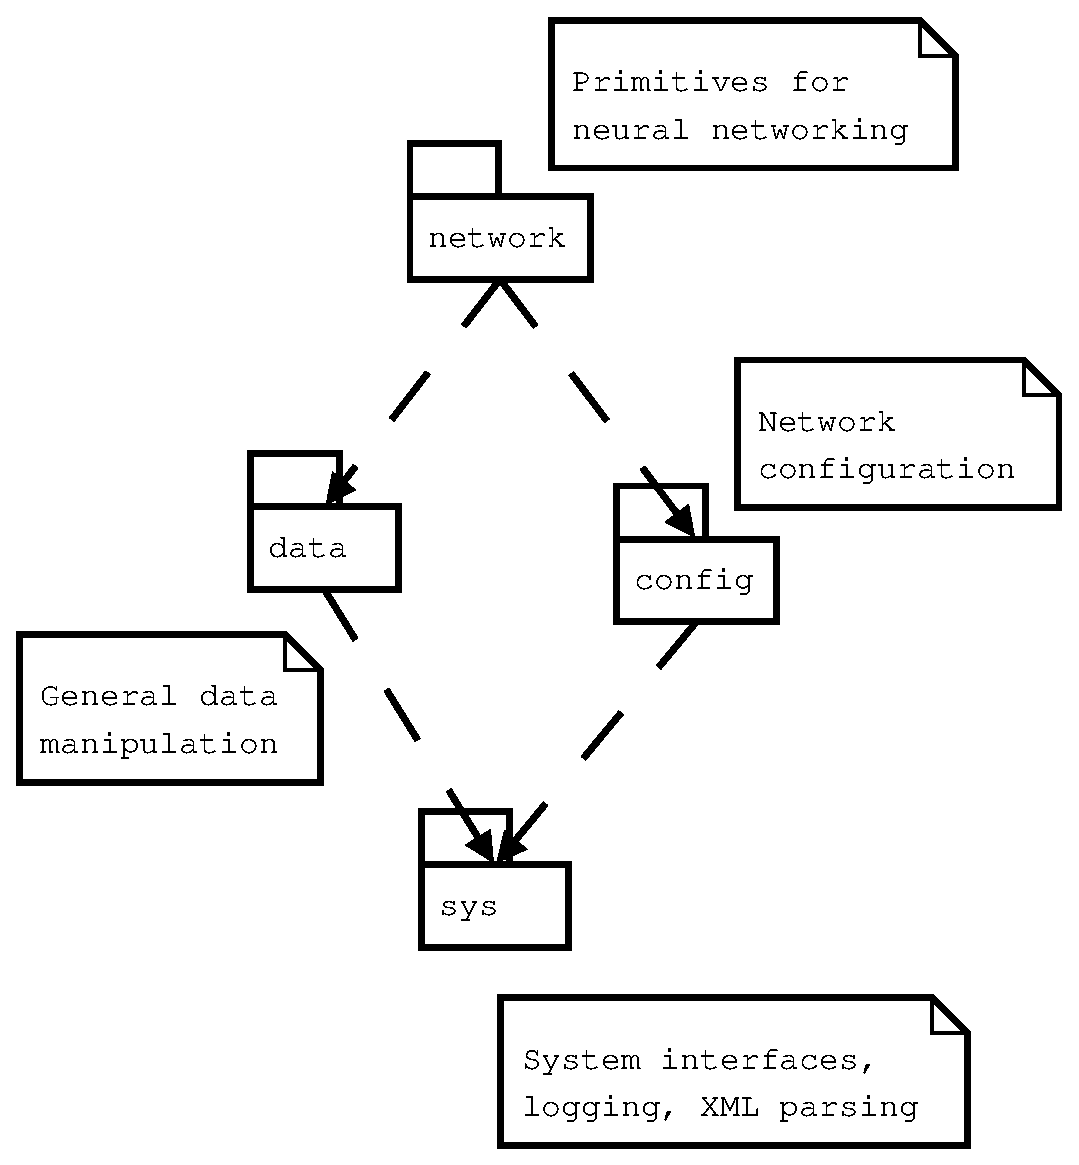
\includegraphics[scale=0.5]{nr-packages}
\end{center}
\caption{Diagrama de blocos mostrando a relação entre os pacotes do
\eng{NeuralRinger}.}
\label{fig:nr-packages}
\end{figure}

\paragraph{\texttt{SYS}:} O sub-pacote \texttt{sys} está abaixo na cadeia de
dependências e não depende de nenhum outro. Este pacote inclui ferramentas
para a manipulação de arquivos no formato XML (do inglês
\eng{eXtensible Markup Language}, \cite{xml}) e um sistema básico para
o relatório de erros. A escolha da linguagem XML como formato de troca de
dados e valores de configuração sucede-se da grande quantidade de
interpretadores (\eng{parsers}) disponíveis livremente na \eng{internet}, já
que é um padrão bastante difundido. O suporte a XML disponível atualmente
inclui, mas não se limita a verificações de sintaxe automatizadas (via
\eng{XML schemas}) e transformações para que se adicione informação ou seja
possível a visualização de forma adequada do conteúdo de uma base de dados
XML.

A Figura~\ref{fig:sys-uml} traz uma visão geral dos componentes e seu
relacionamento dentro deste pacote. Na parte central do diagrama encontra-se o
tipo \texttt{Reporter} que define uma interface para o relatório de
erros. Objetos deste tipo contém uma implementação específica do sistema de
relatório de erros. Inicialmente, somente a implementação baseada em
arquivos-padrão tais como \texttt{std::cout} e \texttt{std::cerr}
\cite{web:gcc-stl} foi desenvolvida. 

À direita observa-se a modelagem para o sistema de interpretadores XML. Uma
interface (abstrata) é utilizada como base para implementações específicas
baseadas em interpretadores habitualmente encontrados nos sistemas
operacionais correntes. Especificamente, implementações para o sistema Xerces
C++ \cite{xerces-c}, do grupo Apache e libxml2 \cite{libxml2}, do grupo Gnome
estão presentes na implementação atual. O interpretador XML utiliza-se do
sistema de relatório de erros para relatar problemas na leitura ou escrita de
arquivos de forma unificada. Uma caixa de ferramentas, baseada no tipo
abstrato \texttt{XMLProcessor} provê um conjunto primitivas para facilitar a
escrita e leitura de parâmetros e trechos de texto. No evento de erros fatais,
uma exceção baseada no tipo \texttt{Exception} será lançada pela parte afetada
do código.

\begin{figure}
\begin{center}
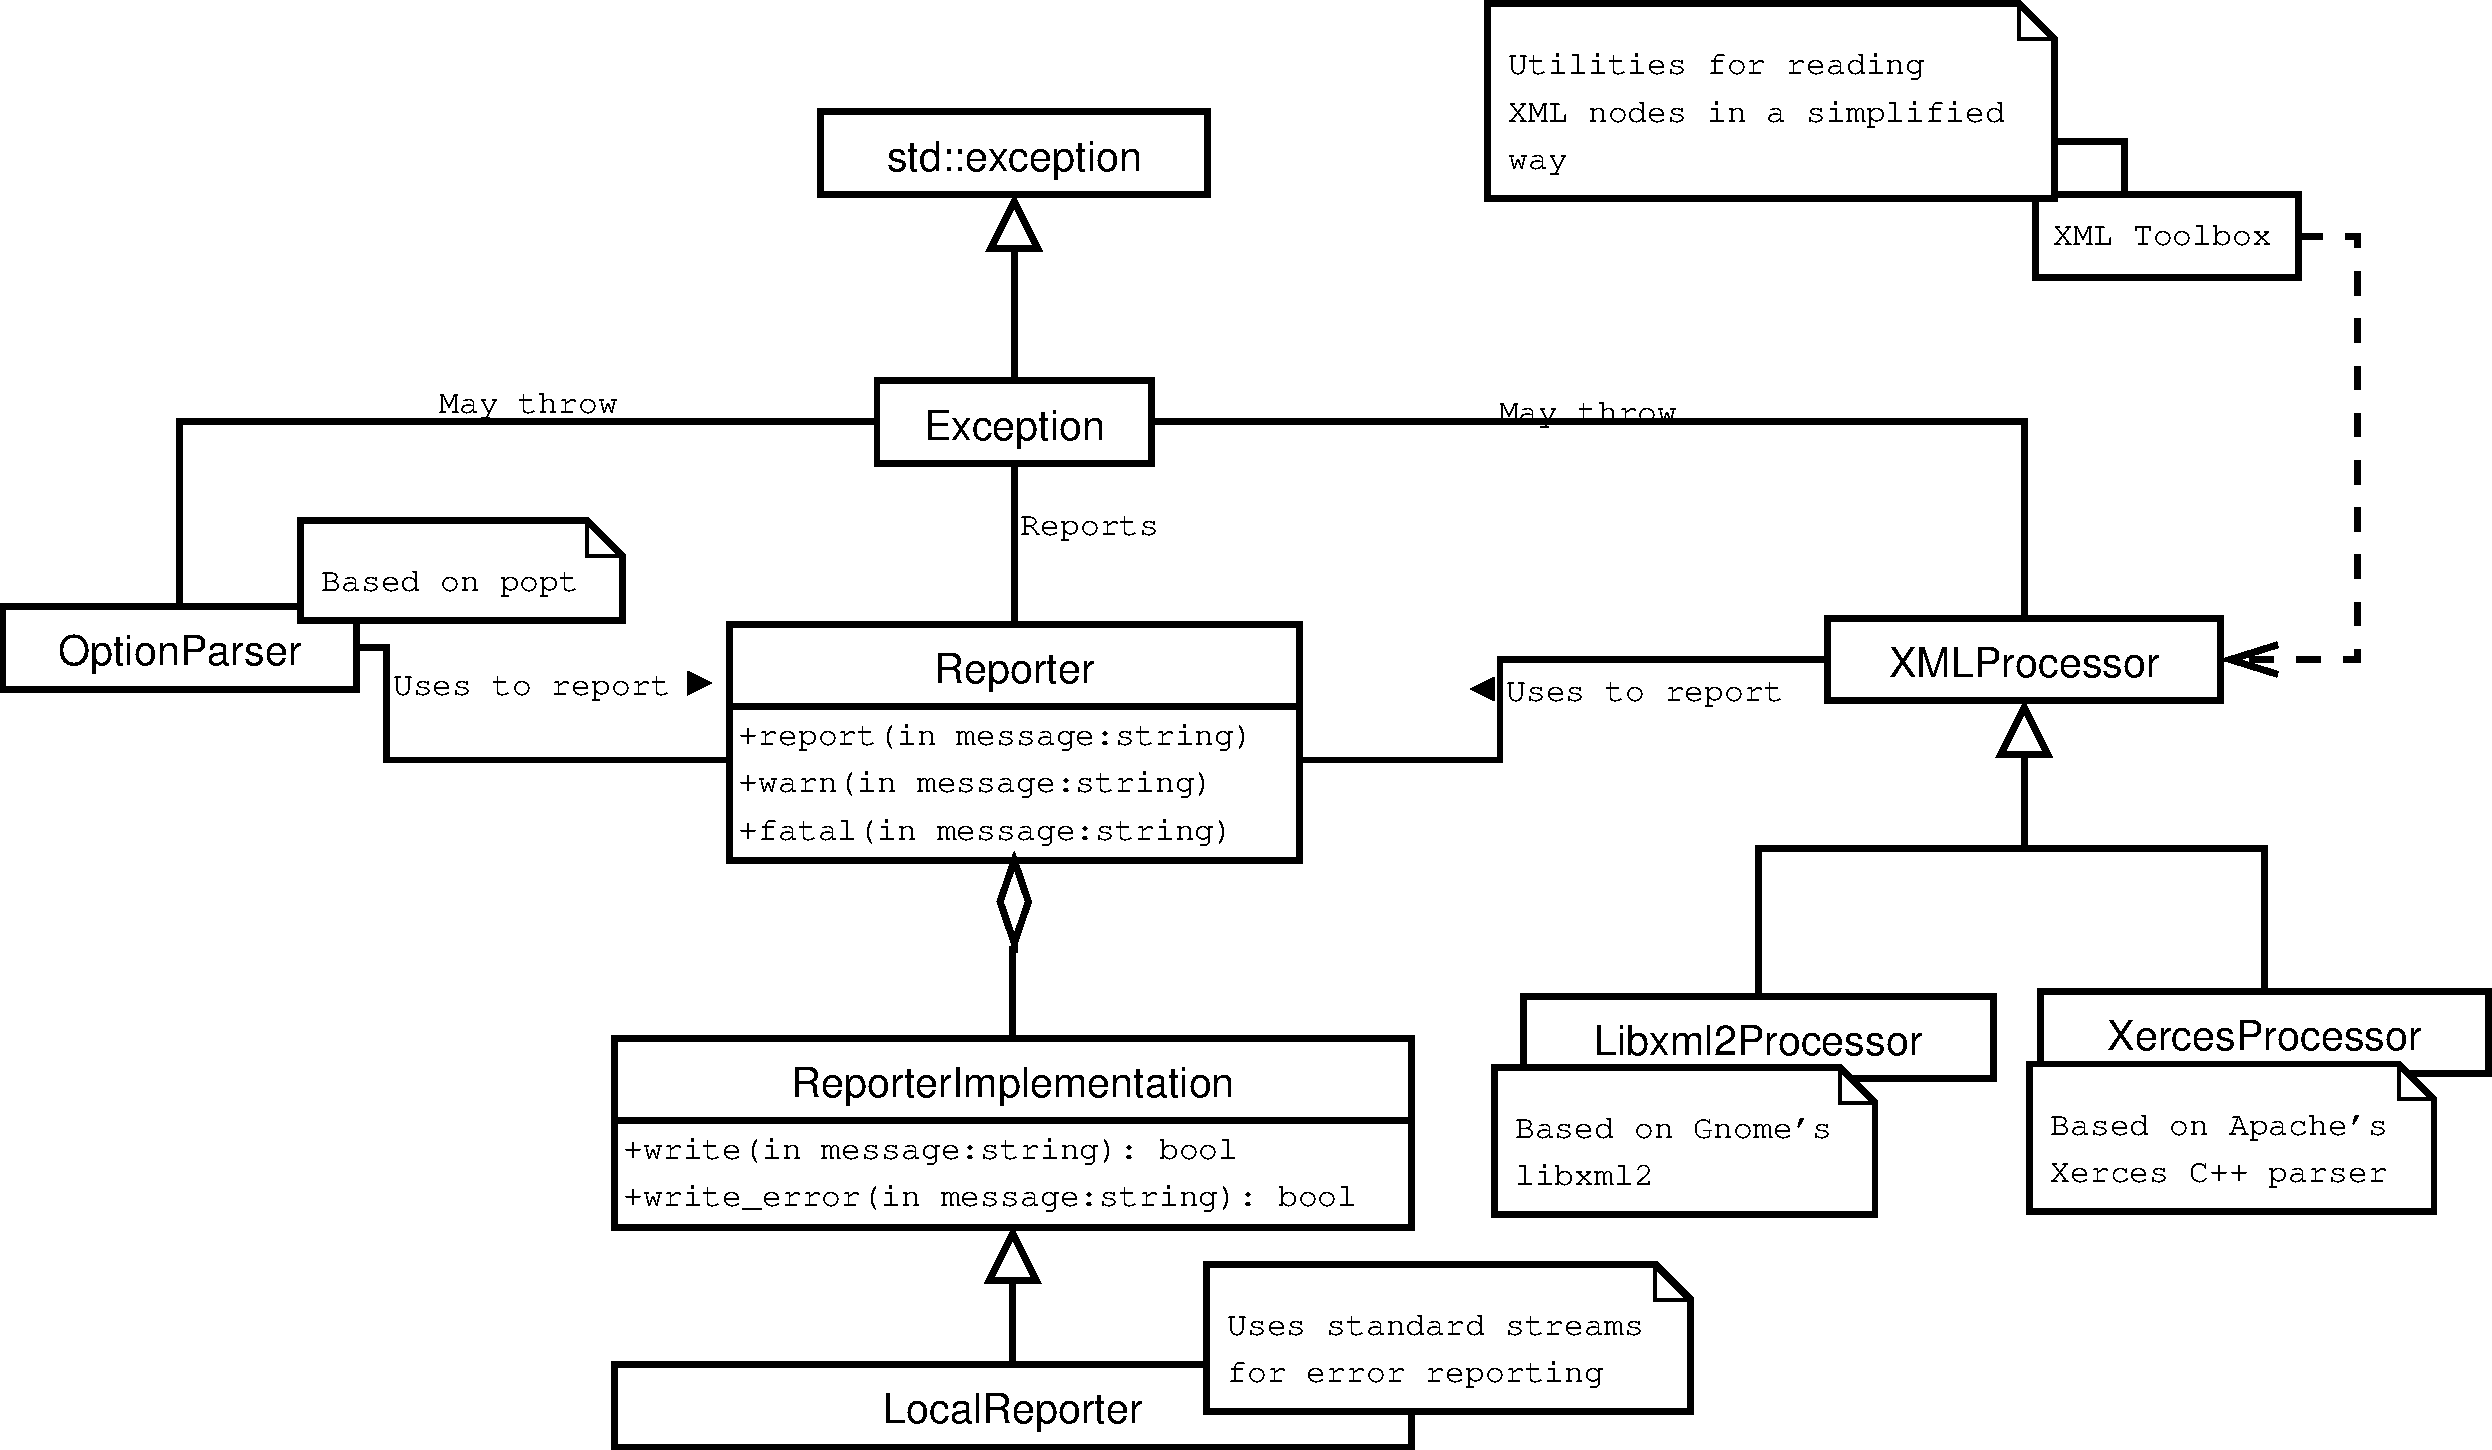
\includegraphics[scale=0.34]{sys-uml}
\end{center}
\caption{Diagrama UML mostrando as relações dos componentes do pacote
\texttt{sys}.}
\label{fig:sys-uml}
\end{figure}

O pacote \texttt{sys} também fornece um sistema para a interpretação de opções
de linha de comando, baseado no interpretador \texttt{popt}. Este tipo imbute
um sistema de atribuição automática e checagem de valores, conectando as
opções na linha de comando diretamente com o contexto onde as opções serão
utilizadas dentro do programa. Seguindo a filosofia dos interpretadores XML,
este tipo também faz uso do sistema central de relatório de erros para
informar problemas ao usuário e poderá, no caso de problemas sérios, também
lançar exceções de operação.

\paragraph{\texttt{DATA}:} O pacote \texttt{data} contém as primitivas para a
manipulação dos dados, prévia e posteriormente ao processamento neural. Este
sub-sistema utiliza-se das primitivas definidas no pacote \texttt{sys} para
executar a reportagem de erros, lançamento de exceções ou a leitura de
arquivos XML. A implementação das primitivas neste pacote utiliza elementos
otimizados da biblioteca GSL (\eng{GNU Scientific Library}, \cite{gsl}) para a
manipulação de valores contidos em matrizes e vetores. A
Figura~\ref{fig:data-uml} contém um diagrama mostrando a relação das classes
dentro do pacote \texttt{data}.

\begin{figure}
\begin{center}
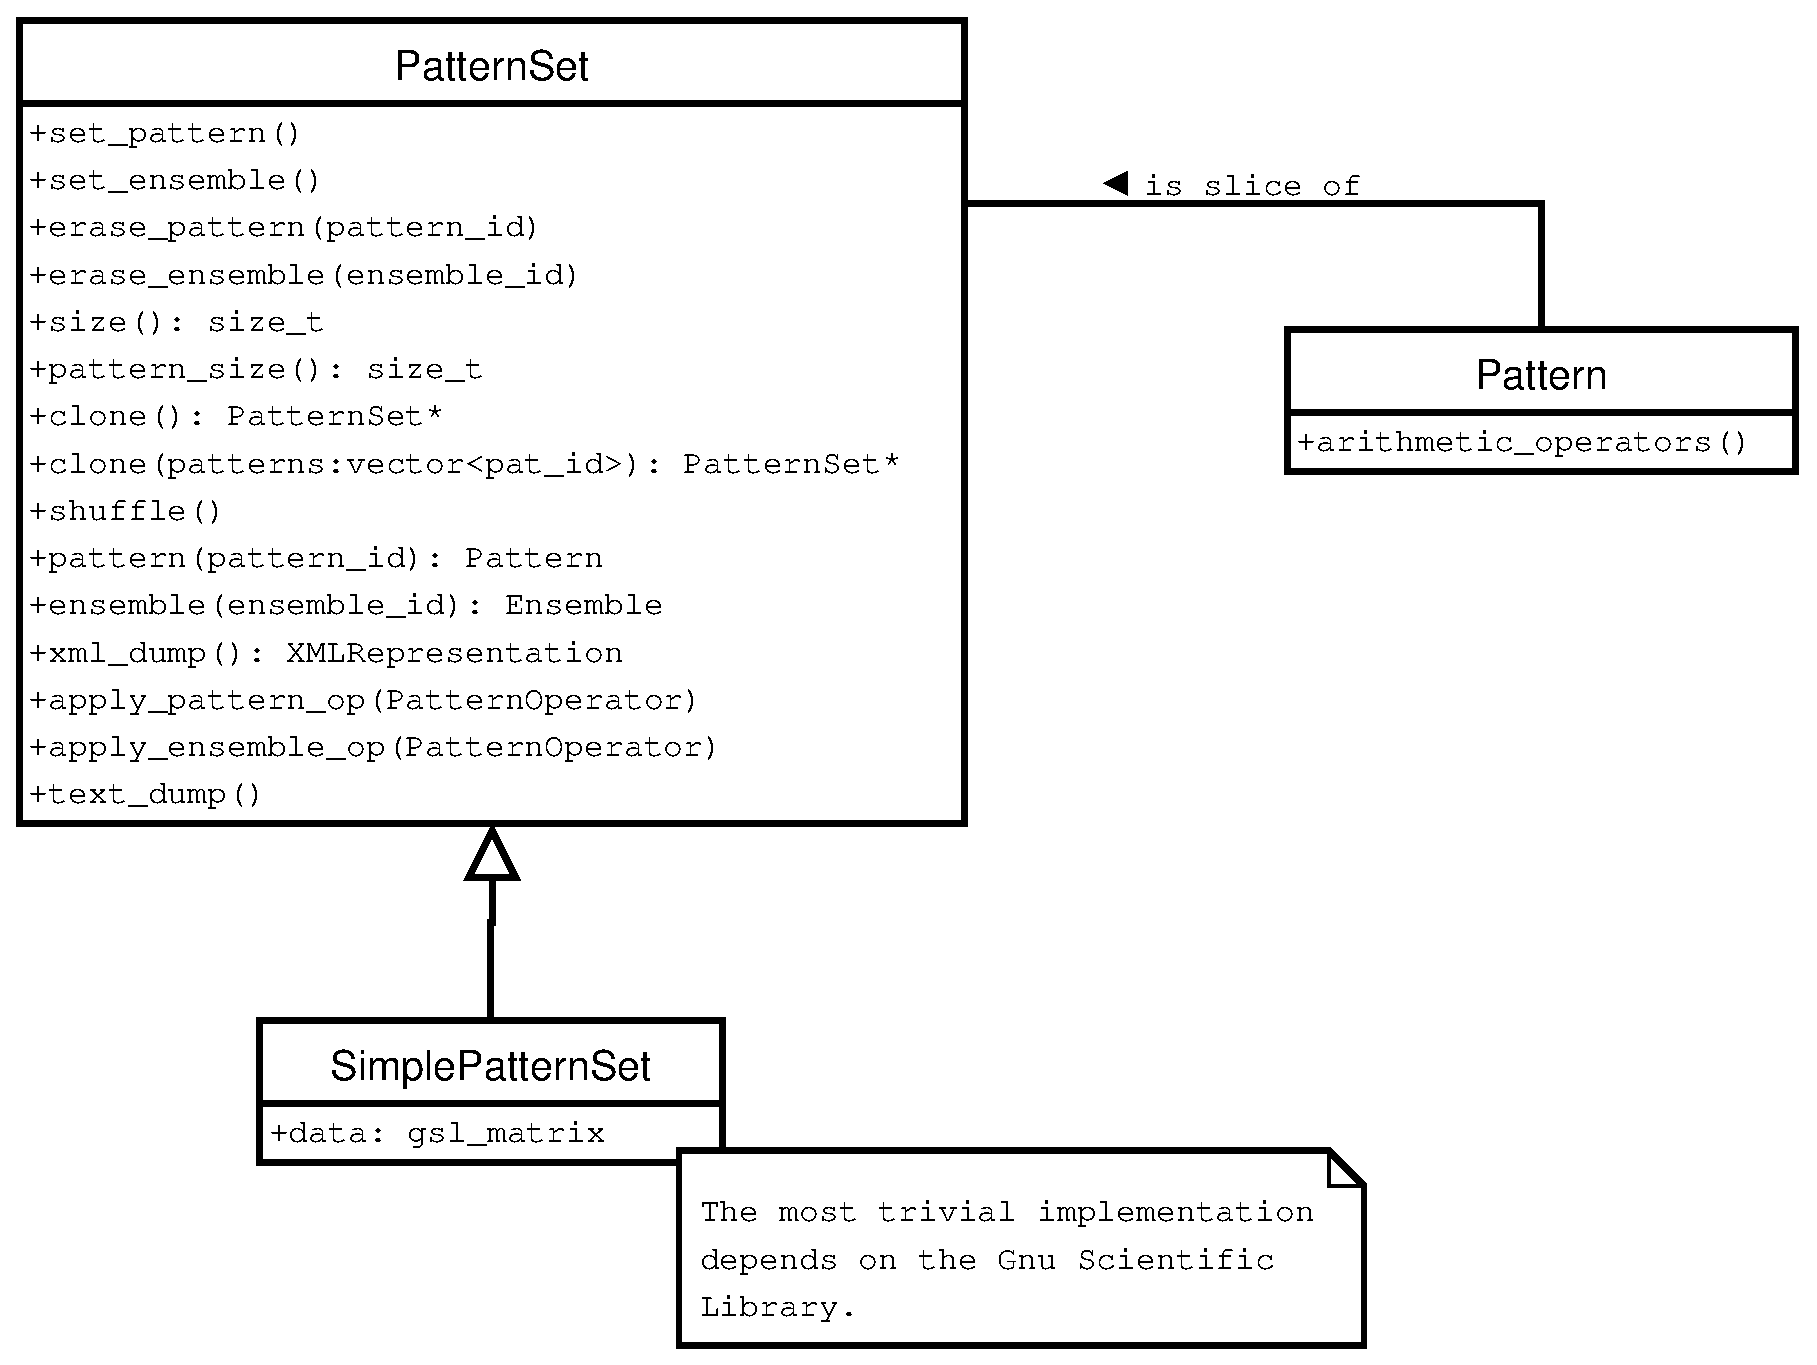
\includegraphics[scale=0.3]{data-uml}
\end{center}
\caption{Diagrama UML mostrando as relações dos componentes do pacote
\texttt{data}.}
\label{fig:data-uml}
\end{figure}

O elemento central deste pacote chama-se \texttt{PatternSet}. Ele representa
um conjunto de vetores ou padrões formando uma matriz de dados. Esta matriz é
representada internamente por um objeto tipo matriz GSL
(\texttt{gsl$\_$matrix}). Para o armazenamento dos dados utilizou-se a seguinte
estratégia: cada evento do fenômeno observado será guardado em uma linha da
matriz. Neste caso, cada coluna representará uma característica (ou
\eng{Feature} no inglês) do dado. A biblioteca GSL permite acesso rápido tanto
aos padrões (linhas) como características (colunas) da matriz de dados. 

Baseando-se nas primitivas de acesso ao tipo matriz GSL, a classe base
\texttt{PatternSet} desenvolve mé\-todos tí\-picos utilizados durante a
manipulação dos dados, tais como acesso simplificado, leitura e escrita em
disco, mistura dos padrões, manipulação de campos específicos e cópia. O
formato de escrita em disco escolhido utiliza o padrão XML. O banco de dados
básico contém um cabeçalho com as informações do autor e dos dados, indicando
a data de criação e última atualização. Dentro do arquivo, os dados podem ser
dividos em classes. Cada classe é dividida por sua vez em padrões, que contém
um número opcional de atributos.

Para o caso específico do processamento de dados de RoIs, uma classe é
derivada da implementação de base de um \texttt{PatternSet}, chamada
\texttt{RoIPatternSet}. Esta classe implementa, adicionalmente à classe de
base, métodos para a salva-guarda, leitura e manipulação de campos
especificamente relacionados a uma RoI assim como os identificadores do
primeiro nível de filtragem e os valores das coordenadas $\eta$ e $\phi$.
Desta forma, é possível correlacionar os resultados obtidos com outros testes
ou com relação ao posicionamento da região de interesse. Exemplos de conjuntos
de padrões são elétrons ou jatos.

Uma coleção de um ou mais conjuntos de padrões é chamada \texttt{Database}, ou
banco de dados. Um banco de dados reúne os diferentes conjuntos de padrões que
se deseja processar através de um mapa. Para cada conjunto de padrões, o
usuário pode atribuir um nome, mapeando os dados propriamente ditos a um valor
legível a uma outra pessoa. Usando um objeto da classe \texttt{Database}, é
possível manipular os conjuntos de padrões de uma forma unificada, por
exemplo, quando deseja-se extrair a média ou desvio padrão global dos
conjuntos de padrões de um problema.

Operadores (\texttt{PatternOperator}s no diagrama), são elementos que podem
modificar um padrão e são usados para extrair a média, variância ou aplicar
normalizações dos mais diferentes critérios nos dados disponíveis. Na figura
mostra-se o mais relevante dos operadores na biblioteca, chamado
\eng{NormalizationOperator}, que é inicializado à partir de uma base de dados
e pode, quando aplicado a um padrão, remover a média e desvio padrão da base
de dados. Este operador é utilizado em todos os testes neste trabalho como
forma de normalização dos dados de entrada de classificadores LMS ou Redes
Neurais. Quando um operator é aplicado a um padrão, primitivas da biblioteca
GSL são utilizadas para que a eficiência do processo seja maximizada.

\paragraph{\texttt{NETWORK}:} Neste pacote contém a definição de
neurônios, sinapses e redes formadas à partir destes elementos. A
Figura~\ref{fig:network-uml} contém um diagrama UML dos tipos neste
sub-sistema. No topo deste diagrama está o tipo \texttt{Network} (Rede), que
representa, de forma abstrata, um conjunto de neurônios (tipo \texttt{Neuron})
interconectados via objetos do tipo sinapse (tipo \texttt{Synapse}). Uma rede
pode ser executada utilizando-se um dos métodos \texttt{run()} e treinada
usando-se uma das variantes de \texttt{train()}. De fato, objetos do tipo
\texttt{Network} não contém nenhuma informação direta sobre a topologia da
rede que executam, funcionando apenas como agentes delegadores de
responsabilidade. O sistema funciona da seguinte forma:

\begin{figure}
\begin{center}
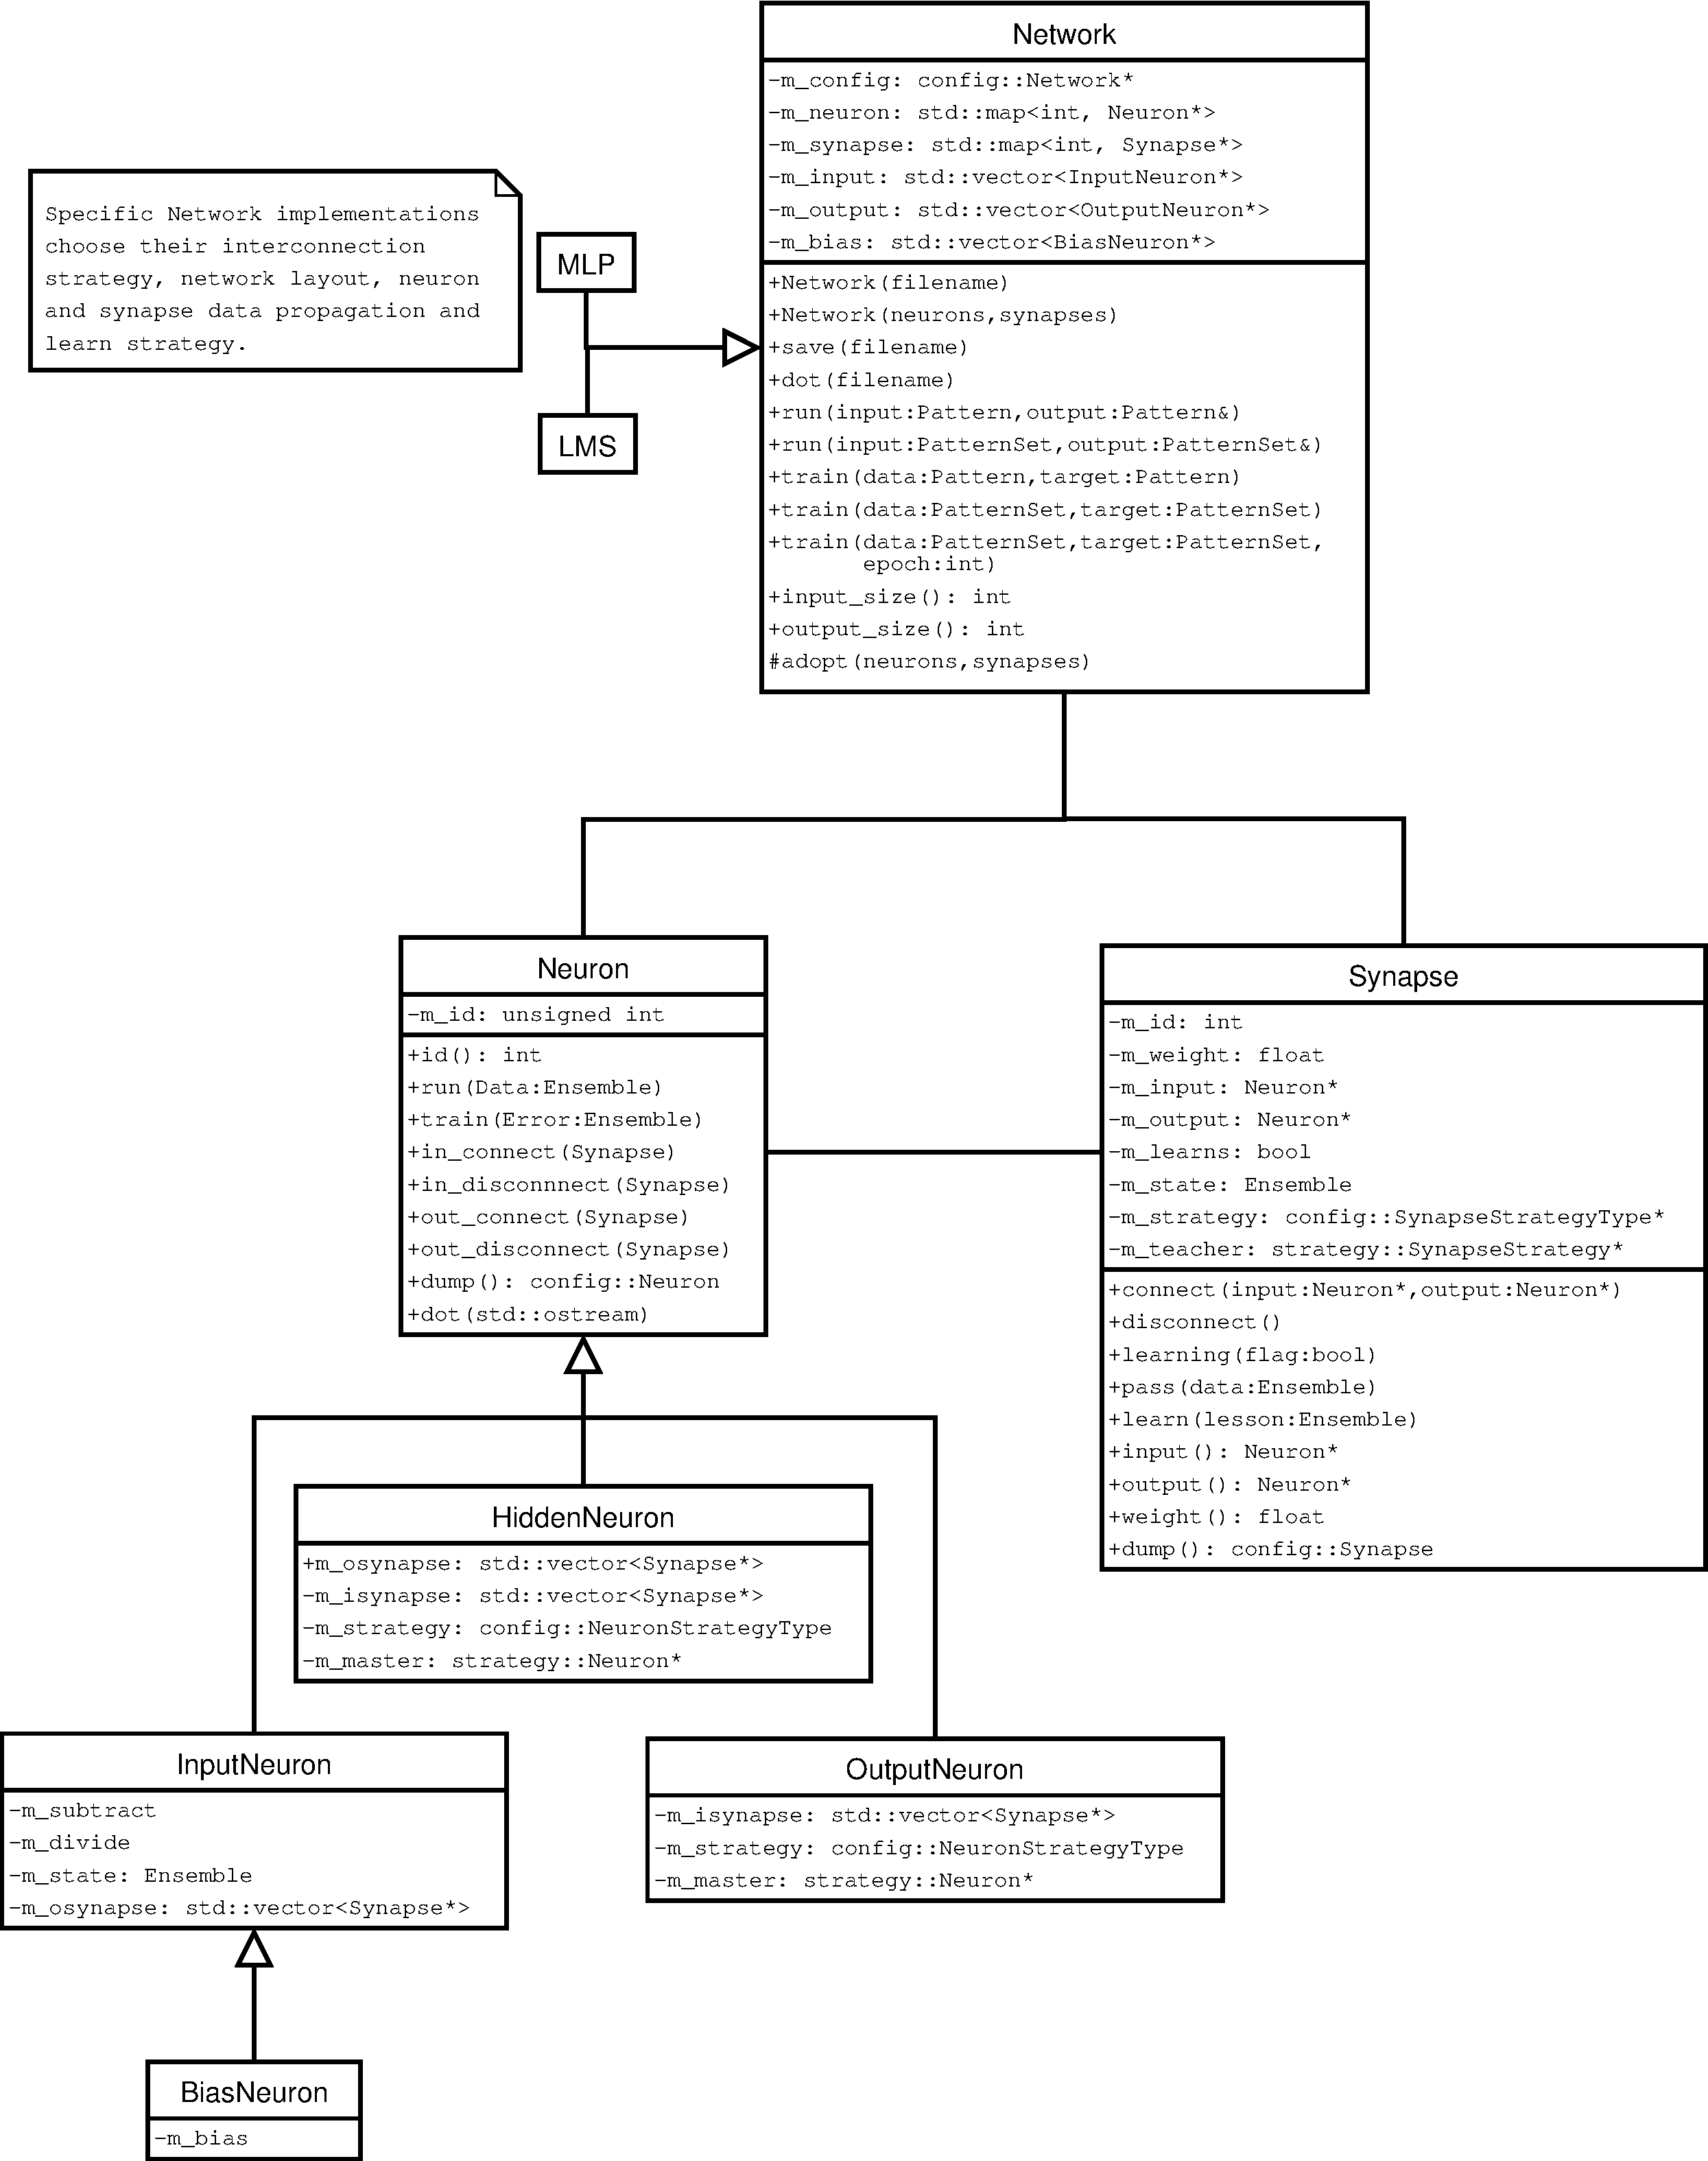
\includegraphics[scale=0.35]{network-uml}
\end{center}
\caption{Diagrama UML mostrando as relações dos componentes do pacote
\texttt{network}.}
\label{fig:network-uml}
\end{figure}

\begin{itemize}
\item \textbf{Para executar a rede}: Neste modo, o usuário irá iniciar o
processo aplicando à entrada da rede um padrão ou conjunto de padrões. O
objeto do tipo \texttt{Network} irá então, para cada coluna da matriz de dados
de entrada, chamar o método \texttt{run()} dos neurônios de entrada,
correlacionando os dados do usuário com as posições relativas do neurônio da
camada de entrada. Opcionalmente, se existirem neurônios de polarização
(\texttt{BiasNeuron}s), o mesmo será feito para cada um destes neurônios. Cada
neurônio de entrada e polarização é responsável por propagar seu sinal aos
neurônios a que está conectado, através das sinapses (objetos do tipo
\texttt{Synapse}). As sinapses irão multiplicar o valor de suas entradas pelo
seu próprio peso e propagar o sinal ao neurônio destino. Este último, após
receber todas as entradas relativas as sinapses que estão conectadas a si,
executará o mesmo procedimento até que o sinal chegue ao neurônio de saída da
rede.

\item \textbf{Para treinar a rede}: O sistema de treinamento funciona de 
modo equivalente. Uma vez calculado o sinal de erro, ou a \textit{lição} à
partir da técnica que convier, este sinal é injetado ao neurônio de saída, que
retropropagará o sinal até o neurônio de entrada.
\end{itemize}

Os tipos de neurônio são divididos nas seguintes classes:

\begin{itemize}
\item Entrada (\texttt{InputNeuron}): são neurônios que recebem a entrada
rede, opcionalmente aplicando um fator de normalização aos dados e propagará o
sinal para neurônios escondidos ou de saída. Como estão no início da rede,
estes neurônios não podem retropropagar sinais recebidos em suas saídas para
fins de treinamento. Uma vez que atingem estes neurônios, os sinais de erro
retropropagados são apagados da memória e o passo de treinamento é considerado
como executado;

\item Polarização (\texttt{BiasNeuron}): este tipo herda suas 
caracte\-rís\-ticas da classe \texttt{In\-put\-Neuron}, mas não permite que o
usu\-á\-rio defina uma entrada arbitrária que será propagada a rede. No lugar,
é possível definir um valor fixo (normalmente $+1$), que é alimentado, via
sinapses de conexão, aos neurônios de saída ou escondidos;

\item Escondido (\texttt{HiddenNeuron}): são neurônios que estão entre os
neurônios de entrada e/ou polarização, conectando a entrada à saída. São
opcionais, já que é possível desenvolver redes sem neurônios desta
classe. Neurônios escondidos transmitem os dados recebidos em suas entradas à
seus neurônios de saída, aplicando uma operação de soma dos valores de
entrada, seguida, opcionalmente de uma função de ativação configurável;

\item Saída (\texttt{OutputNeuron}): são os neurônios que estão na saída da
rede. Seus valores constituem a saída do sistema neural. Assim como os
neurônios escondidos, podem aplicar uma função de ativação ao campo induzido
produzido somando-se os dados de entrada.
\end{itemize}

A execução da rede e treinamento das sinapses é regido por dois parâmetros que
estão atrelados a estes elementos: as estratégias. Estratégias para neurônios
(objetos da classe \texttt{NeuronStrategy}) definem de que forma os neurônios
propagaram os sinais de erro quando são injetados na saída rede, para correção
dos valores sinápticos. No momento, somente há um tipo de stratégia possível:
a retropropagação de erros. Três funções de ativação estão implementadas: a
função linear (utilizada para redes tipo LMS), a função logística
simplificada, definida na Equação~(\ref{eq:logf}) e a função tangente
hiperbólica, definida na Equação~(\ref{eq:tanh}).

Métodos para salva-guardar e restaurar uma rede à partir de um arquivo es\-tão
implementados. A salva-guarda é implementada através de um processo iterativo
de delegação de responsabilidades onde cada neurônio e sinapse involvido na
rede se auto-descreve no arquivo de saída. O formato escolhido é XML, uma vez
que as bibliotecas de base do pacote \texttt{sys} já implementam as primitivas
de leitura e escrita neste formato. Um segundo método (chamado \texttt{dot()})
está disponível para objetos do tipo rede. Este método implementa a
escrita em disco de uma descrição da rede no formato \texttt{dot}
\cite{graphviz}, que permite a visualização dos pesos e interconexões da rede
de forma gráfica. Exemplos de uma rede LMS e uma rede MLP encontram-se nas
Figuras~\ref{fig:lms-dot-example} e ~\ref{fig:mlp-dot-example}
respectivamente. As caixas em verde na parte esquerda da figura representam o
fator de normalização aplicado às entradas. Os círculos azuis, seguindo o
caminho de propagação do sinal representam os neurônios de entrada. Cada
neurônio possui uma numeração única, que o distingue dos outros. Este número
corresponde ao identificador usado dentro das aplicações do
\eng{NeuralRinger}. 

Neurônios escondidos e aqueles pertencentes à camada de saída são
representados por um retângulo com as bordas arredondadas. Neste retângulo, o
identificador do neurônio está representado na parte superior esquerda. Na
parte inferior desta região, abaixo do identificador, um sinal de adição ($+$)
indica que as entradas deste neurônio serão somadas antes da aplicação da
função de ativação, definida na parte esquerda. Nós de polarização são
mostrados junto ao neurônio a que estão conectados. Os diversos neurônios são
conectados por retas que apontam na direção da propagação do sinal de entrada
da rede. A saída da rede é mostrada usando-se um círculo vermelho e localizada
na extrema direita da figura. O número dentro deste círculo corresponde ao
identificar do neurônio de saída e casa com o número indicado no retângulo que
precede o círculo.

\begin{figure}
\begin{center}
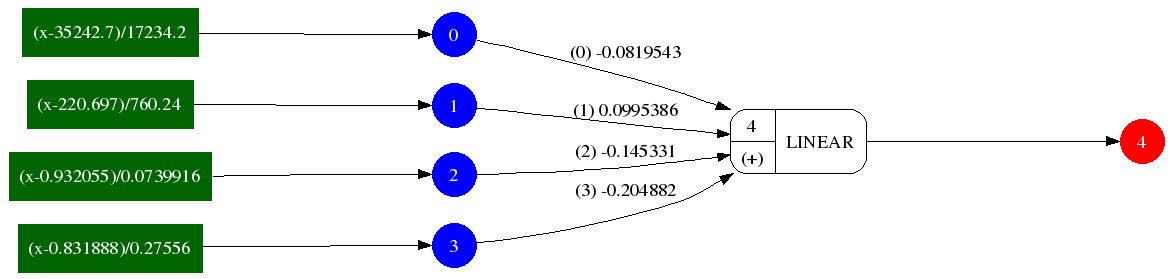
\includegraphics[scale=0.35]{lms-best2}
\end{center}
\caption{Exemplo de uma gráfico de fluxo produzido pelo método \texttt{dot()}
para uma rede LMS, tal qual utilizada para os testes na Seção~\ref{sec:lms}.}
\label{fig:lms-dot-example}
\end{figure}

\begin{figure}
\begin{center}
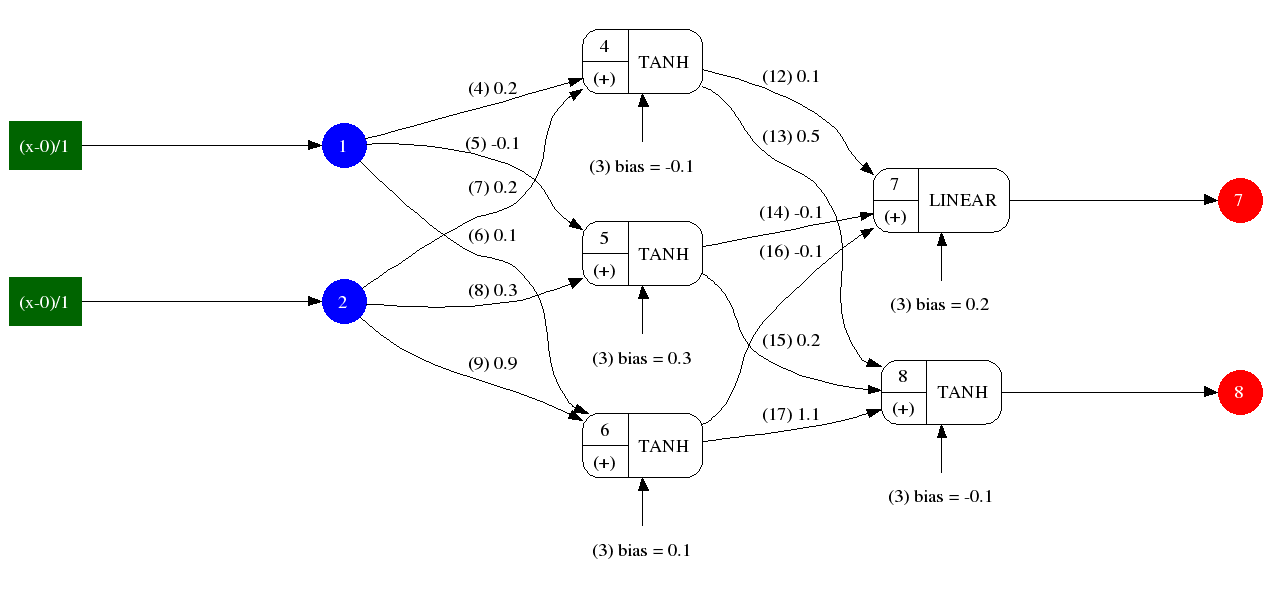
\includegraphics[scale=0.32]{mlp-caloba.png}
\end{center}
\caption{Exemplo de uma gráfico de fluxo produzido pelo método \texttt{dot()}
para uma rede MLP.}
\label{fig:mlp-dot-example}
\end{figure}

\paragraph{\texttt{CONFIG}:} Este pacote implementa a leitura e escrita de
parâmetros de redes a um arquivo XML. É um pacote que depende da
infrasestrutura provida pelo pacote \texttt{sys} e provê suporte a
configuração das redes definidas no pacote \texttt{network}.

\paragraph{Outros pacotes:} O \eng{NeuralRinger} contém, ainda, 3 outros
sub-projetos que apoiam sua funcionalidade:

\begin{itemize}
\item \texttt{lvl1}: contém um simulador simplificado da filtragem baseada em
calorimetria executada no LVL1. Este pacote pode ser utilizado para filtrar,
dentre as regiões de interesse disponíveis, aquelas que seriam aprovadas pelo
LVL1. Ele pode ser usado no lugar de uma simulação completa do Athena para
separar dados para uma análise menos criteriosa. Para o filtro de referência,
é preferível que o usuário utilize o programa Athena;

\item \texttt{roiformat}: define o formato de intercâmbio entre o sistema de
calorimetria implementado no Athena e o \eng{NeuralRinger}, possibilitando que
os dados disponíveis no primeiro, possam ser facilmente escritos em disco e
lidos por versões do \eng{NeuralRinger} não acompladas ao Athena. Isso
normalmente diminui o tempo de desenvolvimento e teste e é aconselhável;

\item \texttt{rbuild}: este pacote contém primitivas para a construções de
anéis baseados nos dados brutos das RoI disponíveis. Este método de deteção é
uma alternativa mais eficaz ao processamento utilizando as características
definidas pelo T2Calo. Este sistema será introduzido mais adiante.
\end{itemize}

\subsubsection{Aplicações:}

Um conjunto de aplicativos foi escrito utilizando o sistema de pacotes
definido na seção anterior. Estes aplicativos podem ser executados
independentemente do sistema Athena, o que simplifica o desenvolvimento e
treinamento das redes neurais, assim como a depuração de eventuais problemas
no código. Estes são os programas disponíveis:

\begin{itemize}

\item \textbf{eta-filter}: Este programa pode sub-dividir uma base de dados
contendo RoIs, de forma a classificar os dados por segmentos em $\eta$. O
programa é iniciado com um arquivo contendo as RoIs no formato XML padrão e
com um valor para $|\Delta_\eta|$. Para cada sub-intervalo de tamanho
$|\Delta_\eta|$ dentro do intervalo $[-2,5, +2,5[$, um arquivo de dados é
gerado. Estes arquivos conterão dados para RoIs nos respectivos intervalos em
$\eta$. O processamento leva em consideração a localização da RoI determinada
pelo LVL1, que está disponível nas bases de dado XML;

\item \textbf{getroi}: Separa RoIs de uma base de dados no formato
\texttt{roiformat} para inspeção por um programa externo;

\item \textbf{lms-train}: Implementa um sistema completo de treinamento 
de uma rede LMS. O sistema é extremamente configurável quanto aos parâmetros de
treinamento, permitindo a especificação da taxa de treinamento, tamanho da
época, critério de parada, tempo de parada abrupta e os nomes dos arquivos de
entrada e saída;

\item \textbf{lvl1-filter}: Este programa implementa um filtro baseado em uma
simulação simplificada do LVL1. Ele pode ser utilizado para filtrar, dentre as
regiões de interesse disponíveis, aquelas que seriam aprovadas pelo LVL1. O
usuário poderá especificar os diversos limites de corte para a filtragem do
primeiro nível:

\begin{itemize}
\item Limite hadrônico;
\item Limite eletromagnético e
\item Isolamento eletromagnético;
\end{itemize}

Assim como está definido na Seção~\ref{sec:lvl2-detect-electron};

\item \textbf{merge}: Este programa pode aglutinar múltiplas bases de dados
XML em um único arquivo de saída; 

\item \textbf{mlp-relevance}: Este programa avalia a relevância das
características de entrada de uma rede (LMS ou MLP), tanto considerando-se o
valor MSE quanto o produto SP originais da rede;

\item \textbf{mlp-run}: Roda uma rede (LMS ou MLP) e escreve uma base de dados
de saída com os resultados;

\item \textbf{mlp-train}: Implementa um sistema completo de treinamento de 
uma rede MLP. De forma análoga ao programa \texttt{lms-train}, esta aplicação
é extremamente configurável quanto aos parâmetros de treinamento, permitindo a
especificação da taxa de treinamento, tamanho da época, critério de parada,
tempo de parada abrupta e os nomes dos arquivos de entrada e saída;

\item \textbf{relevance-filter}: Este programa pode remover uma ou mais
colunas de uma matriz de dados, baseando-se na análise da relevância e um
parâmetro de corte. Com este programa também é possível reduzir o espaço de
entrada de um discriminador, minimizando as perdas na classificação, como será
mostrado mais a frente;

\item \textbf{ringer}: Este programa pode calcular, levando-se em consideração
um padrão de normalização, os anéis de energia que serão utilizados mais a
frente no trabalho. A saída deste programa é uma base de dados no formato XML
padrão do \eng{NeuralRinger};

\item \textbf{ringer-run}: Este programa executa extração e discriminação de
elétrons e jatos baseado na técnica do anelamento a ser descrita nas próximas
seções. Ele pode ser utilizado para o cálculo do desempenho do algoritmo de
filtragem \eng{offline} e permite uma otimização da execução antes da
implementação no ambiente Athena;

\item \textbf{xml2dot}: Escreve a representação de uma rede no formato
\texttt{dot} para que seja possível a visualização tal qual o exemplo das
Figuras~\ref{fig:lms-dot-example} e \ref{fig:mlp-dot-example};

\item \textbf{xml2text}: Este programa converte uma base de dados no formato
XML padrão do \eng{NeuralRinger} em uma representação no formato texto, que
pode ser lido por programas que não suportem XML.
\end{itemize}

Cada um dos programas responde ao command \texttt{--help} que imprime na tela
o conjunto de opções e valores padrões disponíveis. Um conjunto de scripts de
análise é embarcado junto com o pacote permitindo ao usuário a automação do
treinamento e análise dos resultados considerando-se figuras de mérito padrão
para a análise baseada em calorimetria no ATLAS.

\subsection{Discriminação neural aplicada às saídas do T2Calo}

É possível substituir o discriminador LMS definido na Seção{sec:lms} por um
discriminador baseado em uma rede neural tipo MLP como a da
Figura~\ref{fig:simple-mlp}. A implementação desta rede neural foi detalhada
ao longo do capítulo e é facilmente implementável usando o pacote
\eng{NeuralRinger} e o fluxo de treinamento detalhado na
Figura~\ref{fig:train-flow}. A Figura~\ref{fig:t2calo-neural} contém um
diagrama de blocos que ilustra, de forma simplificada, tal sistema. Os fatores
de normalização empregados para o sistema de deteção baseado no algoritmo LMS
não precisam ser substituídos, já que deseja-se empregar o mesmo tipo de
normalização antes de alimentarmos o sistema neural com os dados disponíveis,
a fim de evitar qualquer tipo de tendência devida à variância ou média dos
dados. Os conjuntos de treinamento e teste serão mantidos, o que simplificará
a comparação das duas técnicas.

\begin{figure}
\begin{center}
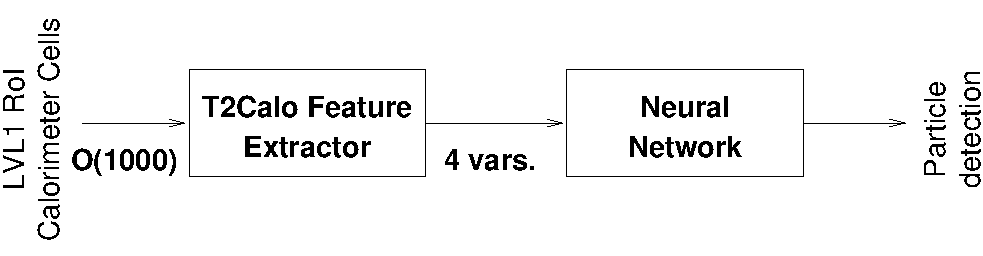
\includegraphics[scale=1]{t2calo-neural}
\end{center}
\caption{Um discriminador neural para as características definidas pelo
T2Calo.}
\label{fig:t2calo-neural}
\end{figure}

Neste novo sistema neural um conjunto maior de parâmetros de treinamento
estará disponível e torna-se necessária a avaliação destes em função do tempo
e qualidade de treinamento das redes. Estes parâmetros são:

\begin{itemize}
\item Taxa de aprendizagem da rede;
\item Tamanho da época;
\item Número de neurônios na camada escondida\footnote{Este estudo
limita-se a utilização de Redes Neurais artificiais com uma única camada
escondida.};
\item Momento.
\end{itemize}

A utilização de um valor de momento tem por objetivo amortecer o treinamento
de forma que a migração para o mínimo da superfície de erro ocorra de forma
suave, e será empregado no caso de observarmos que o treinamento comporta-se
de forma oscilatória. Para cada uma destas variáveis, define-se um conjunto de
sub-valores de interesse:

\begin{itemize}
\item Taxa de aprendizagem: $[0,001; 0,002; 0,005; 0,01; 0,02; 0,05; 0,1;
0,15]$;
\item Tamanho da época: $[50; 100; 200; 500; 1000; 1500]$;
\item Neurônios escondidos: $[2; 3; 4; 5; 6]$;
\item Momento: $[0; 0,01; 0,02; 0,05; 0,1; 0,2]$.
\end{itemize}

Cada conjunto individual de parâmetros deve ser avaliado em função de um
número considerável de pontos de inicialização dos pesos sinápticos da rede
neural. Deseja-se assegurar que as redes convirjam à pontos próximos (se não
idênticos) na superfície de erro considerada, independentemente de sua
inicialização. Estipulou-se que o número de testes para cada conjunto de
parâmetros será 5. Ou seja, para cada ponto no espaço de otimização do
treinamento, conduziremos 5 testes inicializando os pesos sinápticos com
valores aleatórios distintos e disparando o treinamento. Considerar-se-á os
máximos e mínimos obtidos no produto SP do classificador, para o conjunto de
teste, na avaliação de seu desempenho.

Uma inspeção rápida do número de testes a serem executados mostra que, para
este conjunto de parâmetros, cerca de ($8\times6\times5\times6\times5$) 
$7200$ testes devem ser realizados. Embora tentador, este cenário aparenta-se
mais complexo que o problema inicial da otimização do EGammaHypo, com uma
desvantagem: o número de parâmetros aumentou. Uma avaliação mais detalhada da
natureza do espaço de otimização pode ser benéfica a simplificação deste
processo: 

\begin{itemize}
\item Numa análise inicial, é possível suprimir a variação do momento, já que
a contribuição desejada deste parâmetro está no amortecimento do
treinamento. Seria possível adotar a seguinte estratégia: inicialmente
identifica-se a melhor taxa de aprendizagem. Em seguida, estuda-se como
aplicar o momento de forma que o discriminador final seja treinado evitando
transições abruptas do MSE ou do produto SP;

\item O número de neurônios escondidos poderia ser, inicialmente fixado em 4,
igualando o número de entradas. Reconhece-se que um sistema com menos
neurônios escondidos possa apresentar a mesma eficiência ou ainda que um
sistema com mais, convirja mais suavemente. Ainda sim, espera-se que as
tendências no tocante aos outros parâmetros de otimização sejam preservadas e
seja possível identificar o número ótimo de neurônios na camada escondida de
forma \textit{quasi}-independente ao restante dos valores;

\item O tamanho da época pode ser fixado baseando-se na experiência inicial
com o discriminador LMS. O valor utilizado para aquele sistema foi de 500
eventos por época.
\end{itemize}

Desta forma, propõe-se a seguinte heurística de otimização:

\begin{enumerate}
\item Fixa-se todos os parâmetros de treinamento, variando-se a taxa de
aprendizagem em busca de um ótimo para este parâmetro;
\item De posse da taxa de aprendizagem ótima, varia-se o tamanho da época;
\item O número de neurônios escondidos ótimo poderá então ser analisado tendo
em consideração valores ótimos de taxa de aprendizado e o tamanho da época;
\item Por final, varia-se o momento afim de suavizar ao máximo o treinamento
do detetor neural. A utilização de momento será necessária, \textbf{se e
somente se} o treinamento neural se mostrar excessivamente ruidoso.
\end{enumerate}

\subsubsection{Otimização da taxa de aprendizado}

O primeiro parâmetro a ser otimizado, seguindo a heurística proposta é a taxa
de treinamento. Neste caso, 8 valores estão sendo considerados. Para cada um
dos 8 valores, realizou-se 5 testes onde os pesos sinápticos são inicializados
de forma aleatória e distinta. Para cada conjunto de testes relacionados com
um valor fixo de taxa de treinamento, encontra-se a média e o desvio padrão do
produto SP para os conjuntos de treino e teste e do número de passos de
treinamento. Os resultados desta análise podem ser vistos na
Tabela~\ref{tab:t2calo-neural-lr-scan}. O tamanho da época está fixo em 500, o
que indica que, em todos os casos, o sistema teve acesso a um número maior de
padrões que o total disponível para treinamento (cerca de $14500$ padrões,
incluindo elétrons e jatos).

\begin{table}
\begin{center}
\begin{tabular}{|r|r|r|r|} \hline
Tx. de aprendizado & Passos & Prod. SP (treino) & Prod. SP (teste) \\
\hline 
0.0010 & $1339\pm248$ & $1.4935\pm0.0162$ & $1.4943\pm0.0178$ \\ \hline
0.0020 & $1048\pm407$ & $1.4850\pm0.0108$ & $1.4880\pm0.0107$ \\ \hline
0.0050 & $617\pm229$ & $1.4995\pm0.0163$ & $1.4932\pm0.0147$ \\ \hline
0.0100 & $335\pm51$ & $1.4943\pm0.0074$ & $1.4918\pm0.0059$ \\ \hline
0.0200 & $204\pm36$ & $1.5168\pm0.0127$ & $1.5104\pm0.0139$ \\ \hline
0.0500 & $123\pm21$ & $1.5087\pm0.0123$ & $1.5052\pm0.0134$ \\ \hline
0.1000 & $80\pm21$ & $1.5150\pm0.0067$ & $1.5101\pm0.0055$ \\ \hline
0.1500 & $85\pm28$ & $1.5121\pm0.0046$ & $1.5094\pm0.0032$ \\ \hline
\end{tabular}
\end{center}
\caption{Resultados da otimização da taxa de treinamento para um discriminador
neural elétron/jato baseado na saída do T2Calo.}
\label{tab:t2calo-neural-lr-scan}
\end{table}

A tabela mostra que um valor pequeno de taxa de treinamento faz com que a
duração deste processo se extenda demasiado sem, necessariamente compensar em
melhores resultados. Em todos os casos, o sistema parece sempre convergir para
um máximo próximo à 1,50 de produto SP (considerando valores para o conjunto
de teste). Conforme aumenta-se a taxa de treinamento, o número de passos para
a estabilização do sistema diminui, chegando, no caso em que a taxa é igual a
$0,1$, a necessitar apenas de 80 iterações para a convergência. Uma vez que a
média do produto SP apresenta-se maior para o valor de taxa de treinamento
igual a $0,02$, utilizaremos este valor como o valor padrão nas próximas
etapas de otimização.

\subsubsection{Otimização do tamanho da época}

De posse da taxa de aprendizado, é a vez de otimizar-se o tamanho da época,
inicialmente fixa em 500. Os valores de época para o qual deseja-se
experimentar são: $[50; 100; 200; 500; 1000; 1500]$. O mesmo procedimento
utilizado para a otimização da taxa de treinamento será realizado aqui: cinco
testes são realizados para cada tamanho de época. Os resultados destes testes
encontram-se na Tabela~\ref{tab:t2calo-neural-epoch-scan}.

\begin{table}
\begin{center}
\begin{tabular}{|r|r|r|r|} \hline
Padrões por época & Passos & Prod. SP (treino) & Prod. SP (teste) \\
\hline 
50 & $198\pm44$ & $1.5128\pm0.0190$ & $1.5056\pm0.0168$ \\ \hline
100 & $201\pm53$ & $1.5126\pm0.0070$ & $1.5128\pm0.0138$ \\ \hline
200 & $219\pm65$ & $1.5017\pm0.0100$ & $1.5004\pm0.0129$ \\ \hline
500 & $204\pm36$ & $1.5168\pm0.0127$ & $1.5104\pm0.0139$ \\ \hline
1000 & $212\pm34$ & $1.5202\pm0.0167$ & $1.5188\pm0.0121$ \\ \hline
1500 & $185\pm52$ & $1.5083\pm0.0142$ & $1.5051\pm0.0184$ \\ \hline
\end{tabular}
\end{center}
\caption{Resultados da otimização do tamanho da época para um discriminador
neural elétron/jato baseado na saída do T2Calo.}
\label{tab:t2calo-neural-epoch-scan}
\end{table}

Como mostra a tabela, um tamanho de época de $1000$ padrões maximiza a
capacidade discriminante do sistema. O número de iterações não varia
significativamente o que indica que o tempo de treinamento do sistema não está
diretamente correlacionado ao tamanho da época. Utilizar-se-á o valor de
$1000$ como refência na próxima etapa de otimização.

\subsubsection{Otimização do número de neurônios escondidos}

O número de neurônios na camada escondida é a penúltima ou, possivelmente
última etapa na otimização do classificador neural proposto. Neste caso,
utilizaremos os valores pré-estipulados para os dois outros parâmetros: taxa
de treinamento $=0,02$ e tamanho da época de $1000$ padrões. Os valores de
teste são 2, 3, 4, 5 ou 6 neurônios na camada escondida. Mais uma vez, 5
testes são realizados para cada parâmetro e a média e variância do tempo de
treinamento e dos produtos SP é extraída. A
Tabela~\ref{tab:t2calo-neural-hidden-scan} contém os resultados destes testes.

\begin{table}
\begin{center}
\begin{tabular}{|r|r|r|r|} \hline
Número de neur. escondidos & Passos & Prod. SP (treino) &
Prod. SP (teste) \\ \hline 
2 & $259\pm86$ & $1.5086\pm0.0104$ & $1.5078\pm0.0118$ \\ \hline
3 & $178\pm21$ & $1.4967\pm0.0039$ & $1.4921\pm0.0043$ \\ \hline
4 & $212\pm34$ & $1.5202\pm0.0167$ & $1.5188\pm0.0121$ \\ \hline
5 & $173\pm25$ & $1.4982\pm0.0058$ & $1.4941\pm0.0046$ \\ \hline
6 & $198\pm98$ & $1.5025\pm0.0121$ & $1.4986\pm0.0168$ \\ \hline
\end{tabular}
\end{center}
\caption{Resultados da otimização do número de neurônios na camada escondida
para um discriminador neural elétron/jato baseado na saída do T2Calo.}
\label{tab:t2calo-neural-hidden-scan}
\end{table}

Desta tabela, concluímos que o número ótimo de neurônios na camada escondida
deve ser 4. Uma inspeção no desenvolvimento do EMQ e do produto SP nos testes
com os 3 parâmetros de escolha indica que a migração para o mínimo seja suave
e, portanto não seja necessário a aplicação de momento ou qualquer outra
técnica de suavização do treinamento. Em seguida, para confirmar as escolhas,
treina-se um total de 10 redes com os parâmetros selecionados. Os critérios de
parada utilizados são mantidos. Para nos assegurarmos da estabilidade da rede,
deixa-se que a rede treine ainda por cerca de 100 passos depois do ponto de
estabilidade detetado. A Figura~\ref{fig:best-t2calo-mlp-mse} e a
Figura~\ref{fig:best-t2calo-mlp-sp} mostram respectivamente o desenvolvimento,
ao longo do treinamento dos valores EMQ e produto SP para o melhor dos 10
resultados obtidos.

\begin{figure}
\begin{center}
\includegraphics[scale=0.98]{t2calo-mlp/mse-evolution}
\end{center}
\caption{Evolução do EMQ para os conjuntos de treino e teste de um
discriminador elétron/jato neural para as variáveis do T2Calo.}
\label{fig:best-t2calo-mlp-mse}
\end{figure}

\begin{figure}
\begin{center}
\includegraphics[scale=0.98]{t2calo-mlp/sp-evolution}
\end{center}
\caption{Evolução do produto SP para os conjuntos de treino e teste de um
discriminador elétron/jato neural para as variáveis do T2Calo.}
\label{fig:best-t2calo-mlp-sp}
\end{figure}

O sistema estabiliza após cerca de 300 passos, considerando a evolução do
EMQ. No que tange capacidade discriminante, aferida através do produto SP,
após cerca de 100 passos, o sistema parece se tornar irrelevante à contínua
redução do EMQ. A Figura~\ref{fig:best-t2calo-mlp-output} mostra as saídas da
rede, no final do treinamento, para elétrons (em cima) e jatos (em baixo). A
saída para elétrons é fixada em $-1$ e para jatos, em $+1$. Nota-se que,
diferentemente ao sistema LMS, há uma notável separação entre as classes
proporcionada pelo emprego de um discriminador neural. O ponto ótimo de
separação pode ser mais facilmente determinado, inclusive por inspeção
visual. 

\begin{figure}
\begin{center}
\includegraphics[scale=0.98]{t2calo-mlp/test-output}
\end{center}
\caption{Saída para o conjunto de teste, do discriminador neural baseado nas
características extraídas pelo T2Calo.}
\label{fig:best-t2calo-mlp-output}
\end{figure}

Diferentemente do sistema linear baseado no LMS, uma rede neural poderá traçar
uma superfície curva no espaço de entrada (número de dimensões $=4$),
melhorando a separação entre as classes que se deseja detetar. Esta última
figura mostra o resultado desta capacidade discriminativa. Ainda sim, como é
possível inspecionar na Figura~\ref{fig:best-t2calo-test-roc}, a capacidade
discriminante deste algoritmo neural resta bastante próxima à do sistema
baseado num detetor LMS, chegando, em alguns pontos da R.O.C. a ser inferior.

\begin{figure}
\begin{center}
\includegraphics[scale=0.98]{t2calo-mlp/mlp-vs-lms-vs-egamma-roc}
\end{center}
\caption{R.O.C. para o conjunto de teste, do discriminador neural baseado nas
características extraídas pelo T2Calo, comparado com o detetor baseado no LMS
e a técnica de otimização baseado algoritmo EGammaHypo.}
\label{fig:best-t2calo-test-roc}
\end{figure}

O valor do produto SP máximo na curva para o detetor neural está nas
coordenadas onde a deteção de elétrons é igual a $93,25\%$ e o falso-alarme em
jatos é $88,79\%$ ($\approx 2,80$~kHz de falso-alarme). Estes valores
correspondem a um produto SP de $1,51$, tal qual ao caso do discriminador
LMS. Uma verificação das eficiências parcias por região em $\eta$ e em $\phi$
revelam uma estrutura bastante semelhante aos sistemas de deteção precedentes,
como mostram as Figuras~\ref{fig:best-t2calo-test-sp-eta} e
\ref{fig:best-t2calo-test-sp-phi}. 

\begin{figure}
\begin{center}
\includegraphics[scale=0.98]{t2calo-mlp/test-sp-eta}
\end{center}
\caption{Análise do produto SP ao longo de $\eta$ para o discriminador neural
baseado nas saídas do T2Calo.}
\label{fig:best-t2calo-test-sp-eta}
\end{figure}

\begin{figure}
\begin{center}
\includegraphics[scale=0.98]{t2calo-mlp/test-sp-phi}
\end{center}
\caption{Análise do produto SP ao longo de $\phi$ para o discriminador neural
baseado nas saídas do T2Calo.}
\label{fig:best-t2calo-test-sp-phi}
\end{figure}

A Figura~\ref{fig:best-t2calo-test-sp-emet} mostra o valor relativo do produto
SP for faixa de energia transversa na seção e.m.. Um comparativo entre os 3
métodos do produto SP por faixas de energia descritos até agora se segue
na Figura~\ref{fig:best-t2calo-versus-others-emet}. Os dados nesta figura
correspondem aos do conjunto de teste, para um corte efetuado em $-0.273$ para
o discriminador neural, e para os melhores resultados obtidos com os outros
dois sistemas de deteção de forma equivalente.

\begin{figure}
\begin{center}
\includegraphics[scale=0.98]{t2calo-mlp/test-sp-emet}
\end{center}
\caption{Análise do produto SP ao longo de $E^{e.m.}_T$ para o discriminador
neural baseado nas saídas do T2Calo.}
\label{fig:best-t2calo-test-sp-emet}
\end{figure}

\begin{figure}
\begin{center}
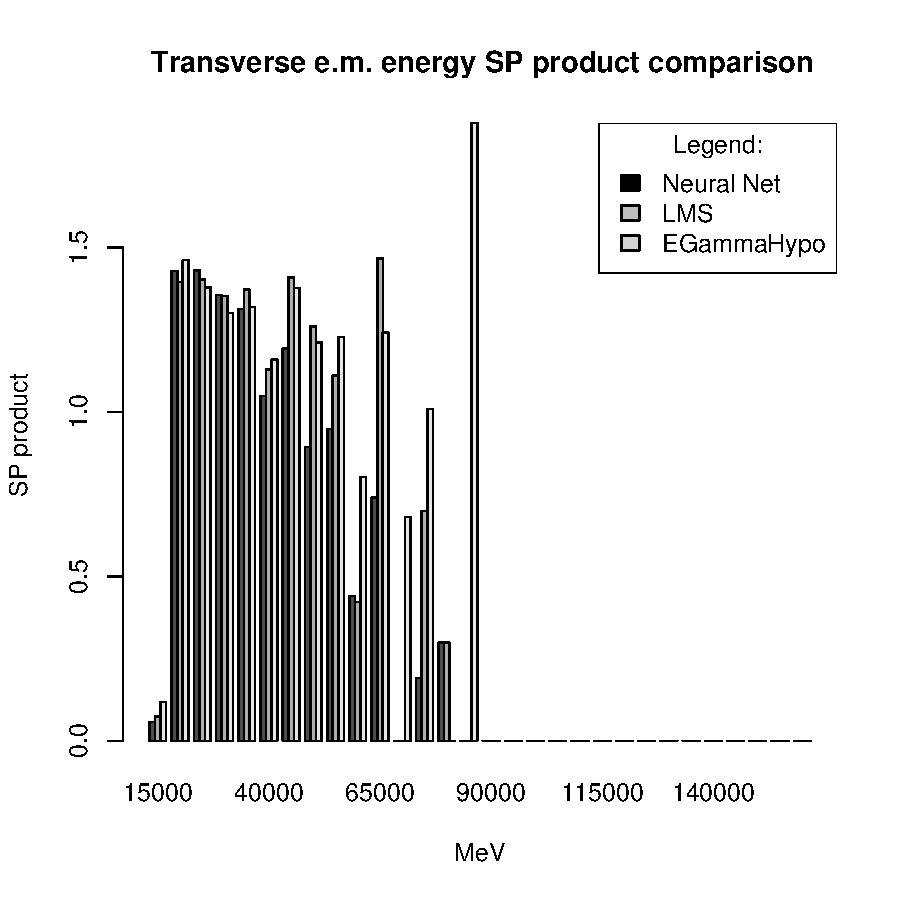
\includegraphics[scale=0.98]{t2calo-mlp/mlp-vs-lms-vs-egamma-et}
\end{center}
\caption{Comparativo do produto SP para os 3 detetores abordados até aqui, por
faixa de energia e.m. transversa.}
\label{fig:best-t2calo-versus-others-emet}
\end{figure}

É possível notar que o sistema neural ganha nas faixas energéticas onde há
mais eventos, porém apresenta uma eficiência marginalmente mais baixa conforme
a energia na seção e.m. aumenta. Num geral, os três sistemas possuem
características bastante próximas nesta análise, concordando entre si. As
análises de relevância, tanto baseadas no EMQ quanto no valor máximo do
produto SP encontram-se nas Figuras~\ref{fig:best-t2calo-mse-relevance} e
\ref{fig:best-t2calo-sp-relevance}. A primeira análise (EMQ) nota-se que há
concordãncia, resguardadas as diferenças nos padrões de saída em cada um dos
casos, na relevância de cada característica neste quesito. O método neural, no
entanto, acentua a falta de importância da componente hadrônica na saída da
rede. Na análise de relevância baseada no máximo do produto SP nota-se que a
ordem de relevância está alterada. Na primeira análise, a variável $\rcore$
parece ser a mais importante, seguindo-se das variáveis $\eratio$, $\ethad$ e
finalmente $\etem$. Baseando-se na variação do produto SP, a variável mais
importante na discriminação é $\eratio$, seguindo-se então de $\rcore$,
$\ethad$ e $\etem$. Diferentemente do sistema linear, as três mais importantes
variáveis de discriminação possuem valores de relevância relativamente
próximos (nos arredores de $0,10$ para $\etem$, $0,15$ para $\rcore$ e $0,20$
para $\eratio$). No sistema linear, a relevância na deteção é fortemente
encabeçada pela variável $\rcore$, com as outras variáveis cerca de uma ordem
de magnitude menos relevantes. 

Um outro ponto observável na análise baseada na variação do produto SP é que,
para o conjunto de treino, a variável $\etem$ possui relevância de
discriminação negativa, encontrando-se aproximadamente em $-0,005$. Este
resultado indica que esta variável estaria atrapalhando o processo de deteção.
Porém, uma vez que seu valor homólogo para o conjunto de teste tenha valor
positivo, nas mesmas proporções, assume-se que este resultado advém,
possivelmente, de uma flutuação estatística e não representa uma real
tendência da variável em questão. Observando os valores de relevância baseados
na diferença do produto SP para os outros 9 testes realizados para o mesmo
conjunto de parâmetros de treinamento, nota-se que esta tendência repete-se em
apenas alguns dos testes, reforçando a conclusão de que este resultado se
trataria apenas de uma flutuação estatística.

\begin{figure}
\begin{center}
\includegraphics[scale=0.98]{t2calo-mlp/relevance-mse}
\end{center}
\caption{Os valores de relevância para os conjunto de treino
(cinza claro) e teste (em cinza escuro), para as 4 variáveis do T2Calo e
considerando-se o classificador neural em estudo.}
\label{fig:best-t2calo-mse-relevance}
\end{figure}

\begin{figure}
\begin{center}
\includegraphics[scale=0.98]{t2calo-mlp/relevance-sp}
\end{center}
\caption{Os valores de relevância de discriminação para os conjunto de treino
(cinza claro) e teste (em cinza escuro), para as 4 variáveis do T2Calo e
considerando-se o classificador neural em estudo.}
\label{fig:best-t2calo-sp-relevance}
\end{figure}

Estas análises também indicam que, tendo por base conjunto de variáveis do
T2Calo, as classes de elétrons e jatos sejam linearmente separáveis. Este
resultado é bastante natural, dado que este conjunto de características tenha
sido otimizado para uma análise baseada em cortes definidos por um operador
experimentado. A Figura~\ref{fig:t2calo-mlp-best-net} mostra uma representação
discriminador neural discutido até agora, para fins ilustrativos. Na próxima
seção definiremos um novo tipo de extração de características que terá por
objetivo maximizar a deteção de elétrons e jatos.

\begin{figure}
\begin{center}
\begin{sideways}
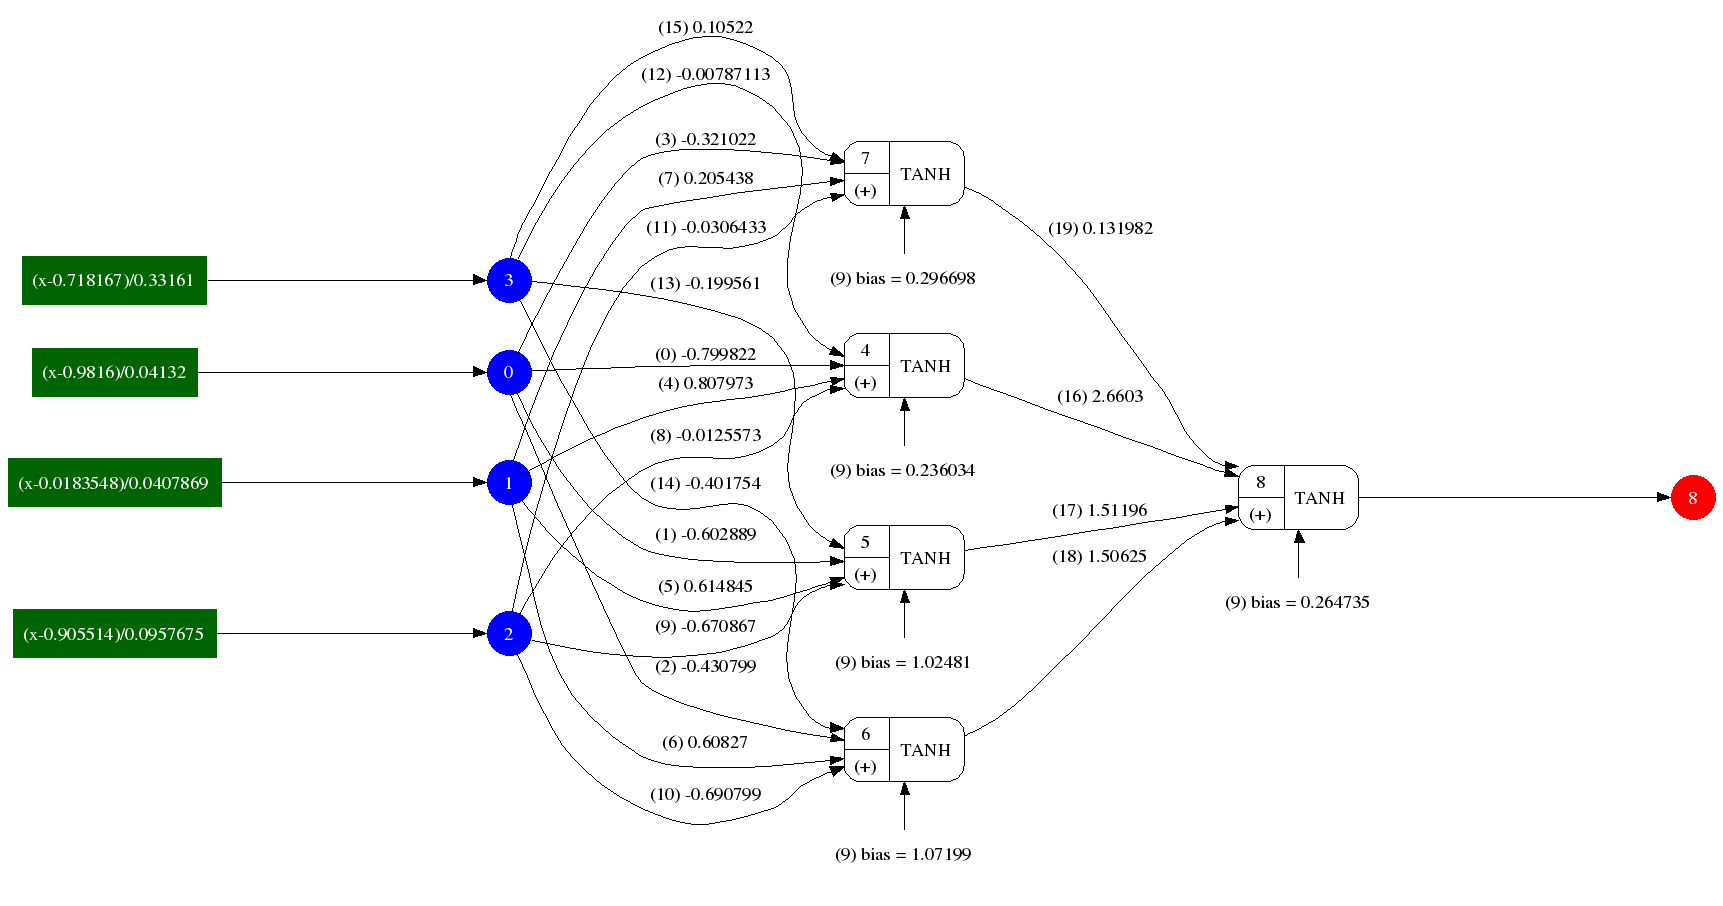
\includegraphics[scale=0.30]{t2calo-mlp/mlp-end}
\end{sideways}
\end{center}
\caption{Diagrama de fluxo do sistema de deteção elétron/jato, neural, usando as
características do T2Calo como entrada.}
\label{fig:t2calo-mlp-best-net}
\end{figure}

\section{Mapeamento topológico}

O algoritmo T2Calo, durante a análise conduzida no LVL2, compacta a informação
da RoI representando um candidato à elétron em quatro quantidades altamente
discrimantes. Tendo estes valores por base obteve-se os seguintes resultados:

\begin{enumerate}
\item Para o EGammaHypo, $91,85\%$ de eficiência na deteção de elétrons contra
$10,19\%$ de falso alarme em jatos;
\item Para detetor LMS, $91,64\%$ para elétrons contra $9,35\%$ de falso alarme;
\item Para uma rede neural, $93,25\%$ para elétrons contra $11,21\%$ de falso
alarme.
\end{enumerate}

Embora as técnicas (LMS e MLP) propostas sejam mais robustas quanto à operação
e manutenção, a qualidade física da separação não é tão afetada. Isto se deve,
principalmente, à agressiva compressão nos dados proporcionada pelo algoritmo
de extração de características. Ainda que não seja viável a deteção de objetos
usando toda a informação da RoI (cerca de 1300 células), é possível encontrar
um método que se situe a meio caminho entre este dois extremos.

Nesta seção, propõe-se um método de compactação da informação da RoI que
utiliza a topologia do evento para gerar um conjunto de características que
pode ser usado para atingir maiores eficiências de deteção de elétrons e
menores valores de falso-alarme.

\subsection{Topologia de uma RoI e anelamento}

Observando-se a interação de elétrons e jatos (enquanto falsos-elétrons) com
os calorímetros, é possível assumir que estes objetos interagirão de forma
aproximadamente isotrópica em relação ao eixo $\eta$ do detetor. Ou seja, dado
um ponto de impacto inicial, a partícula tende a decair em objetos menos
energéticos ao redor do eixo de penetração. Este fenômeno ocorrerá de forma
expansiva, formando finalmente um cone de deposição energética, como o
exemplificado na Figura~\ref{fig:cone}.

\begin{figure}
\begin{center}
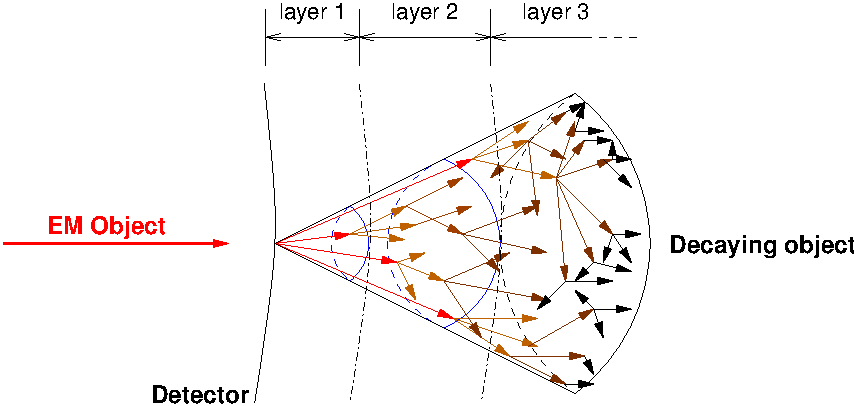
\includegraphics{msc/cone}
\end{center}
\caption{Modelo de um objeto e.m. interagindo com um calorímetro.}
\label{fig:cone}
\end{figure}

A Figura~\ref{fig:electron-roi} mostra um gráfico com a deposição energética na
segunda camada e.m. de uma RoI proveniente de um elétron simulado. As partes
acinzentadas indicam deposição energética, enquanto que as partes em branco
indicam que houve pouca ou nenhuma deposição energética na região.

\begin{figure}
\begin{center}
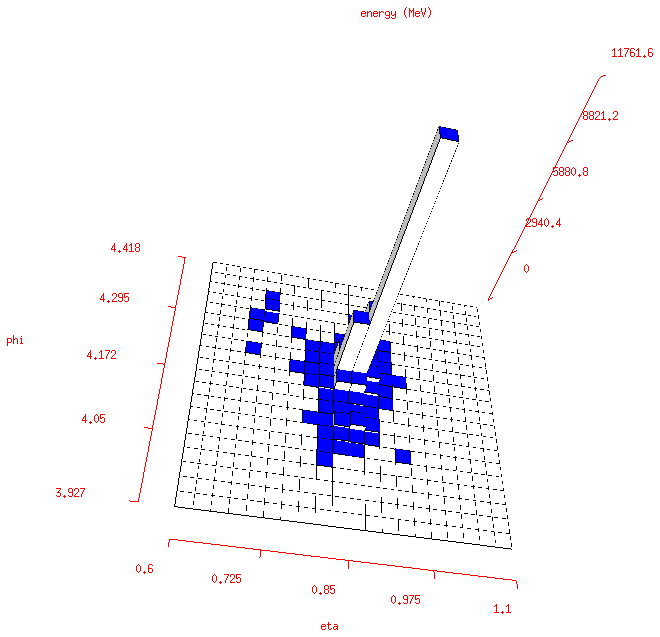
\includegraphics[scale=0.6]{roi-em2}
\end{center}
\caption{Imagem tri-dimensional mostrando o padrão de deposição energética de
um elétron simulado na segunda camada e.m. do calorímetro do ATLAS.}
\label{fig:electron-roi}
\end{figure}

Como colocado na Seção~\ref{sec:e-detection}, a topologia da interação do
objeto em análise com os calorímetros define, com boa margem de sucesso o tipo
do mesmo. Elétrons tendem a um menor espalhamento que jatos, percorrendo
menores distâncias ao longo do eixo $\eta$. Por outro lado, jatos tendem a
radializar a deposição energética, formando cones mais largos e possivelmente
mais profundos.

Levando-se em consideração a formatação dos calorímetros do ATLAS e sua
granularidade, sugere-se o seguinte algoritmo de compactação:

\begin{description}
\item[\ding{182}] Define-se, para cada camada, o centro de posição
energética. Isto é feito de forma simplificada, procurando para todas as
células dentro de uma mesma camada, aquela célula com maior deposição
energética;
\item[\ding{183}] Uma vez que o centro de interação esteja definido, formar um
conjunto de anéis com formato retangular que circumdem este pico. A largura
destes anéis é ajustada de forma que a largura do anel de energia seja a mesma
que de uma célula dentro da camada estudada;
\item[\ding{184}] Para cada anel, somar os valores energéticos das células que
recaem sobre o seu interior.
\end{description}

A Figura~\ref{fig:rings} esquematiza tal algoritmo. Nesta figura encontram-se
exemplos de anéis de energia formados em 4 diferentes camadas dos calorímetros
do detetor ATLAS. Próximo ao centro da RoI, nota-se uma célula que destaca,
hipoteticamente, o centro de deposição energética que a etapa \ding{182} do
algoritmo encontraria. Em seguida, as células de cada segmento são somadas
para a obtenção das ``características'' do objeto a ser discriminado.

\begin{figure}
\begin{center}
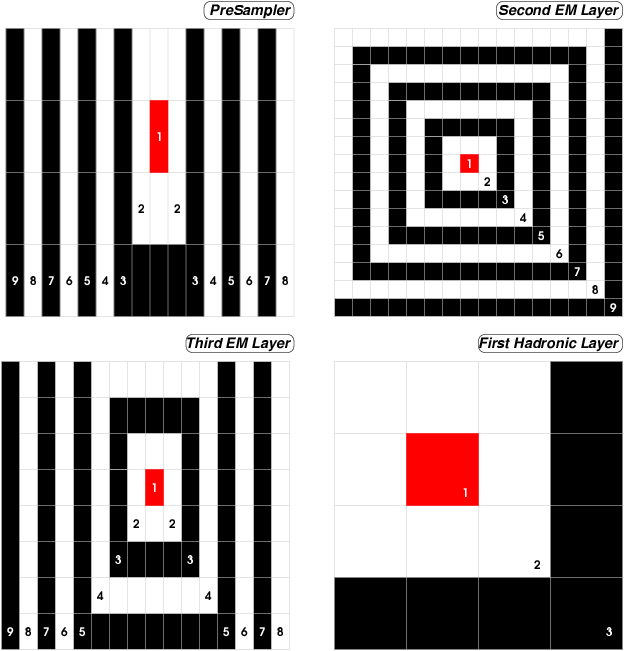
\includegraphics[scale=0.5]{msc/rings}
\end{center}
\caption{Esquematização do processo de anelamento para as diferentes camadas
dos calorímetros do ATLAS.}
\label{fig:rings}
\end{figure}

A granularidade dos anéis respeita a granularidade \emph{típica} das células
na camada. Sabe-se, no entanto, que a granularidade das células varia com
$\eta$ no detetor. Nos casos onde a granularidade é diferente da granularidade
padrão na camada, atribuir-se-á a energia da célula ao anel onde recai o
centro da mesma. Este algoritmo também é resiliente à dados
faltantes\footnote{Ocorrendo, potencialmente, com a falha de um canal de
leitura ou do sistema de aquisição de dados.}, uma vez que células que não
puderem ser lidas apenas não serão contabilizadas. Isto evita procedimentos de
verificação especiais que poderiam comprometer o desempenho do algoritmo de
compactação proposto. Através desta figura observa-se igualmente que algumas
camadas, devido ao formato não simétrico das células (maiores numa direção que
na outra), terão anéis abertos ou incompletos. Desta forma, marcou-se
segmentos que pertencem ao mesmo anel com um número indicando a que anel
determinado segmento pertence.

Um problema recorrente nos algoritmos de filtragem do ATLAS é a região de
\eng{wrap-around} da variável $\phi$, já que o detetor tem formato
cilíndrico. Um cuidado especial deve ser tomado na confecção dos anéis,
levando-se em consideração que, por exemplo, a região com $\phi = 6,18$ está
bastante próxima a região com $\phi = 0,1$, apesar da diferença
numérica. Outro problema encontrado é que diferentes partes do sistema de
localização dos dados dentro do Athena identificam a região do detetor onde
$\phi > \pi$ de maneiras distintas. Para parte do código (relativa à seção
e.m.), o detetor se encontra na área entre $[-\pi, \pi]$ enquanto que para
outra (parte hadrônica), o detetor se encontra na área entre $[0, 2\pi]$. Para
resolver este problema, implementou-se um algoritmo que normaliza as
diferenças em ambos os casos.

Ademais, por se tratar de elétrons ou jatos na qualidade de falsos-elétrons, é
bastante provável que a relação sinal-ruído seja pequena nas camadas traseiras
do detetor, principalmente na região hadrônica. A Figura~\ref{fig:roi-had-9}
mostra a deposição energética de um elétron na primeira camada do detetor
hardrônico. Nesta figura este fenômeno pode ser bem observado.

\begin{figure}
\begin{center}
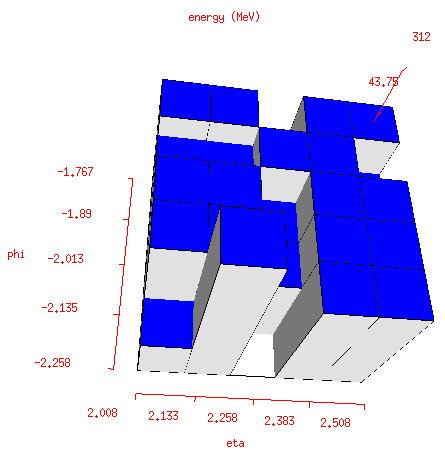
\includegraphics[scale=0.6]{roi-had-9}
\end{center}
\caption{Imagem tri-dimensional mostrando o padrão de deposição energética de
um elétron simulado na primeria camada hadrônica do calorímetro do ATLAS.}
\label{fig:roi-had-9}
\end{figure}

Para evitar que o ruído inerente à eletrônica do detetor possa interferir com
o aferimento do centro de deposição energética, a procura do pico em uma
camada está restrita a uma região de $\eta=0,1\times\phi=0,1$ ao redor do pico
de deposição na segunda camada e.m.. Como já colocado um capítulo anterior
deste trabalho, a segunda camada e.m. é a mais profunda do sistema de
calorimetria, concentrando a maior parte da energia dos elétrons que interagem
com este detetor. Desta forma, se há um pico de deposição energética, este é
considerado para a formação dos anéis. De outra maneira, um ponto aleatório
(aquele com maior energia) dentro da sub-janela definida pelo pico de
deposição energética na segunda camada e.m. é escolhido.

Tomando-se em consideração a granularidade padrão de todas as camadas do
calorímetro (7 no total, incluindo o pré-irradiador), a configuração sugerida
para o número de anéis pode ser encontrada na Tabela~\ref{tab:ring-config}. O
número de anéis em cada camada leva em consideração o número máximo de anéis
que podem ser formados considerando-se uma sub-região de $0,4 \times 0,4$ no
plano $\eta\times\phi$. É interessante notar que nem sempre esta região
cobrirá completamente uma região do mesmo tamanho, já que o posicionamento dos
anéis depende do centro de deposição energética em cada camada. No entanto,
como podemos ver no exemplo do T2Calo, uma região de $0,3 \times 0,3$ está
garantida ao redor do pico de energia, o que é suficiente para a análise de
elétrons \cite{daqnote00-02}.

\begin{table}
\begin{center}
\begin{tabular}{>{\bfseries}l r r r}
Camada & Número de Anéis & Larg. do anel ($\eta$) & Larg. do anel ($\phi$) \\ \hline
Pré-irradiador & 8 & $0,025$ & $\frac{\pi}{32} \approx 0,098174$ \\ 
1\eira\ e.m. & 64 & $0,0031245$ & $\frac{\pi}{32} \approx 0,098174$ \\ 
2\eira\ e.m. & 8 & $0,025$ & $\frac{\pi}{128} \approx 0,024544$ \\ 
3\eira\ e.m. & 8 & $0,05$ & $\frac{\pi}{128} \approx 0,024544$ \\ 
1\eira\ hadrônica & 4 & $0,1$ & $\frac{\pi}{32} \approx 0,098174$ \\ 
2\eira\ hadrônica & 4 & $0,1$ & $\frac{\pi}{32} \approx 0,098174$ \\ 
3\eira\ hadrônica & 4 & $0,1$ & $\frac{\pi}{32} \approx 0,098174$ \\ \hline
Total & 100 & & \\ \hline
\end{tabular}
\end{center}
\caption{Configuração para os anéis formados à partir de uma RoI de tamanho
$\eta = 0,4 \times \phi = 0,4$.}
\label{tab:ring-config}
\end{table}

Um total de $100$ anéis forma o conjunto de entrada para o novo sistema de
discriminação elétron/jato. Nota-se que o primeiro anel de cada conjunto será
considerado o pico de deposição energética na camada. Para classificar os
padrões neste espaço de alta dimensionalidade, utilizaremos detetores baseados
em redes neurais tipo MLP como descrito nas seções anteriores.

\subsubsection{Normalização}

Uma vez que estaremos lidando com os diferenciais energéticos dentro da mesma
camada, por muitas vezes sutis, faz-se necessário que a normalização aplicada
aos conjuntos de anéis seja compatível com a deteção destas
diferenças. Ademais, outros estudos \cite{seixas:pca} já demonstraram que a
informação periférica dentro de cada camada de uma RoI é tão ou mais
importante à discriminação que a quantidade de energia depositada no pico. Por
estas razões, neste trabalho propomos um sistema de normalização dos dados da
RoI baseado em um conjunto de razões cujo o denominador diminui, de forma
relacionada a energia na camada, do centro para as bordas da região de
interesse. Desta forma, o pico de deposição energética na camada (ou
``primeiro anel'') teria um fator de normalização maior que o segundo anel,
que seria por sua vez maior que o fator de normalização aplicado ao terceiro
anel e, assim, sucessivamente. O algoritmo está descrito matematicamente na
Tabela~\ref{tab:seq}.

\begin{table}
\renewcommand{\baselinestretch}{1}
\begin{center}
\begin{tabular}{>{\bfseries}l r r}
Anel & Normalização & Soma em anel \\ \hline
1 & $E$ (total da camada) & $E_1$\\
2 & $E - E_1$ & $E_2$ \\
3 & $E - E_1 - E_2$ & $E_3$\\
4 & $E - E_1 - E_2 - E_3$ & $E_4$\\
\dots  & \dots \\
N-4 & $E - E_1 - E_2 - ... - E_{N-5}$ & $E_{N-4}$ \\
N-3 & $E - E_1 - E_2 - ... - E_{N-5} - E_{N-4}$ & $E_{N-3}$ \\
N-2 & $E - E_1 - E_2 - ... - E_{N-5} - E_{N-4}$ & $E_{N-2}$ \\
N-1 & $E - E_1 - E_2 - ... - E_{N-5} - E_{N-4}$ & $E_{N-1}$ \\
N & $E - E_1 - E_2 - ... - E_{N-5} - E_{N-4}$ & $E_N$ \\
\end{tabular}
\end{center}
\renewcommand{\baselinestretch}{1.5}
\caption{Algoritmo para a ``Normalização Seqüencial''.}
\label{tab:seq}
\end{table}

Neste algoritmo, o primeiro anel (pico de deposição energética) será
normalizado pelo valor da energia total na camada. O segundo anel pelo valor
da camada subtraindo-se o valor de deposição energética no primeiro anel. O
terceiro anel, pelo valor da energia na camada menos o valor do primeiro e
segundo aneís e desta forma, recursivamente até que todos os anéis estejam
normalizados. Nos referiremos à este algoritmo à partir de agora como
algoritmo de ``Normalização Seqüencial''.

Nota-se que este tipo de normalização poderá amplificar em demasiado os
valores periféricos. Isto é desejável para os anéis que se sucedem ao pico de
energia na camada, porém nem tanto para os anéis da periferia da RoI, onde a
relação sinal-ruído é praticamente nula. Desta forma, propõe-se que, à partir
de um determinado limiar de energia, o fator de normalização torne-se
constante. Desta forma evita-se que o sinal ruidoso das bordas influencie o
sistema de discriminação de maneira significativa.

O sub-pacote \texttt{rbuild} do \eng{NeuralRinger} contém a implementação de
referência para este processo de anelamento descrito. Ademais, este pacote
pode ser re-configurado de forma a definir a largura dos aneis de cada camada
ou o número máximo de anéis por camada. Assim, o sistema de anelamento torna-se
independente do tamanho real da RoI e, portanto, independente de quão completo
são os dados recebidos pelo processador do LVL2. Anéis sem dados recebem o
valor \eng{default} que é igual a zero. O formato do arquivo de configuração é
também em XML, o que simplifica a leitura e escrita dentro do contexto do
projeto.

\subsubsection{Dados}

Os dados utilizados nas seções anteriores não podem ser re-utilizados para
esta porção do projeto, uma vez que é necessita-se do acesso aos dados
``brutos'' da RoI. Em outras palavras, deseja-se acesso aos mesmos dados
utilizados pelo T2Calo para a operação de extração de características que este
algoritmo realiza. De posse destes dados, é possível definir a operação de
compactção topológica proposta. A Figura~\ref{fig:datagen} mostra o sistema
que foi utilizado para a obtenção dos dados. Para cada RoI que é analisada
pelo T2Cal, um conjunto de células é carregado dos arquivos de dados
iniciais. Em seguida, os valores das células são calibrados e mapeados na
geometria do detetor de forma que possam ser mais facilmente acessados pelo
algoritmo de extração de características. À partir deste ponto, o T2Calo tem
acesso aos dados e, é exatamente neste ponto que inserimos um \eng{patch}, que
permite que os valores das células ``vistas'' pelo algoritmo sejam guardadas
em um arquivo separado.

\begin{figure}
\begin{center}
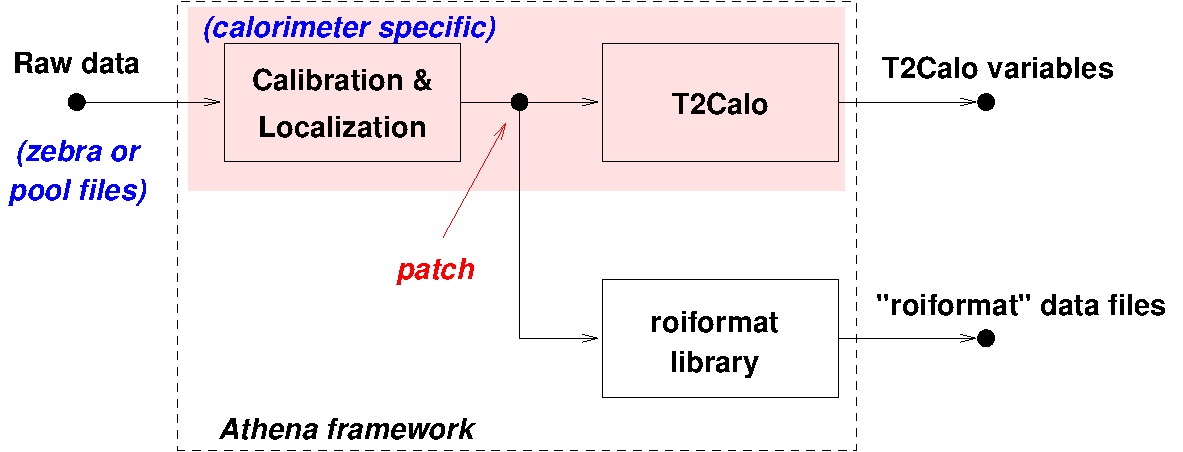
\includegraphics[scale=0.74]{datagen}
\end{center}
\caption{Estratégia para obter acesso aos dados tais quais processados pelo
algoritmo T2Calo.}
\label{fig:datagen}
\end{figure}

O formato deste arquivo é legível pelo sub-pacote \texttt{roiformat} do
\eng{NeuralRinger} e pode ser transformado em uma base de dados de anéis
utilizando-se o programa \texttt{ringer}, descrito anteriormente. Desta forma,
criou-se uma base de dados à partir do mesmo conjunto de eventos analisados na
caracterização do desempenho físico do T2Calo. Esta nova base de dados tem
cerca de $30000$ eventos com a mesma proveniência e características dos
eventos analisados até o momento.

\subsection{Discriminação baseada em anelamento}

O processo de anelamento reduz o espaço de dados de entrada em uma RoI (cerca de
1300 células) para 100 valores correspondes aos anéis formados com os dados
das 7 camadas dos calorímetros. Sería difícil conceber um sistema de
discriminação simples como o proposto para o EGammaHypo neste caso, uma vez
que a possibilidade de combinações é muito grande. Neste caso, adota-se um
sistema de discriminação neural, conectado à saída do sistema de anelamento que
executará o processo de deteção.

Tal qual nos sistemas anteriores, executou-se uma rápida análise do espaço dos
parâmetros de treinamento neural. A Tabela~\ref{tab:ringer-param-optimization}
resume os resultados e indica os valores de taxa de treinamento, tamanho da
época e número de neurônios escondidos utilizados. Para cada tripla destes
parâmetros, 5 testes foram executados e o resultado exposto na tabela
representa a média e desvio padrões levando-se em consideração estas 5
instâncias.

\begin{table}
\begin{center}
\renewcommand{\baselinestretch}{1.0}
{\tiny
\begin{tabular}{|l|l|l|r|r|r|} \hline
\rottext{Tx. de Aprendizado} & \rottext{Tamanho da Época} & \rottext{Neurônios escondidos} & \rottext{Número de iterações} & \rottext{Produto SP (treino)} & \rottext{Produto SP (teste)} \\ \hline \hline

0.0100 & 100 & 4 & $356\pm78$ & $1.6329\pm0.0149$ & $1.6199\pm0.0156$ \\ \hline
0.0100 & 100 & 6 & $372\pm88$ & $1.6237\pm0.0247$ & $1.6202\pm0.0183$ \\ \hline
0.0100 & 100 & 8 & $280\pm39$ & $1.5987\pm0.0210$ & $1.6017\pm0.0215$ \\ \hline
0.0100 & 100 & 10 & $337\pm58$ & $1.6263\pm0.0385$ & $1.6137\pm0.0320$ \\ \hline
0.0100 & 200 & 4 & $366\pm43$ & $1.6119\pm0.0335$ & $1.5986\pm0.0302$ \\ \hline
0.0100 & 200 & 6 & $299\pm33$ & $1.5961\pm0.0236$ & $1.5945\pm0.0264$ \\ \hline
0.0100 & 200 & 8 & $340\pm62$ & $1.6246\pm0.0250$ & $1.6144\pm0.0221$ \\ \hline
0.0100 & 200 & 10 & $287\pm75$ & $1.5994\pm0.0444$ & $1.5968\pm0.0342$ \\ \hline
0.0100 & 500 & 4 & $285\pm64$ & $1.5914\pm0.0211$ & $1.5880\pm0.0225$ \\ \hline
0.0100 & 500 & 6 & $296\pm53$ & $1.6061\pm0.0251$ & $1.5998\pm0.0200$ \\ \hline
0.0100 & 500 & 8 & $254\pm56$ & $1.5981\pm0.0165$ & $1.5937\pm0.0156$ \\ \hline
0.0100 & 500 & 10 & $343\pm68$ & $1.6177\pm0.0273$ & $1.6120\pm0.0225$ \\ \hline
0.0100 & 1000 & 4 & $250\pm44$ & $1.5974\pm0.0215$ & $1.5897\pm0.0183$ \\ \hline
0.0100 & 1000 & 6 & $260\pm24$ & $1.5999\pm0.0307$ & $1.5998\pm0.0201$ \\ \hline
0.0100 & 1000 & 8 & $267\pm41$ & $1.6024\pm0.0175$ & $1.5934\pm0.0193$ \\ \hline
0.0100 & 1000 & 10 & $271\pm46$ & $1.5876\pm0.0182$ & $1.5863\pm0.0164$ \\ \hline

0.0200 & 100 & 4 & $460\pm106$ & $1.7245\pm0.0227$ & $1.6928\pm0.0200$ \\ \hline
0.0200 & 100 & 6 & $347\pm57$ & $1.7056\pm0.0141$ & $1.6774\pm0.0176$ \\ \hline
0.0200 & 100 & 8 & $421\pm78$ & $1.7215\pm0.0163$ & $1.6920\pm0.0149$ \\ \hline
0.0200 & 100 & 10 & $366\pm80$ & $1.7120\pm0.0208$ & $1.6888\pm0.0179$ \\ \hline
0.0200 & 200 & 4 & $265\pm67$ & $1.6716\pm0.0333$ & $1.6549\pm0.0265$ \\ \hline
0.0200 & 200 & 6 & $315\pm72$ & $1.6893\pm0.0192$ & $1.6688\pm0.0147$ \\ \hline
0.0200 & 200 & 8 & $283\pm57$ & $1.6870\pm0.0154$ & $1.6627\pm0.0156$ \\ \hline
0.0200 & 200 & 10 & $301\pm58$ & $1.6903\pm0.0268$ & $1.6662\pm0.0197$ \\ \hline
0.0200 & 500 & 4 & $351\pm42$ & $1.7028\pm0.0094$ & $1.6774\pm0.0098$ \\ \hline
0.0200 & 500 & 6 & $348\pm61$ & $1.6941\pm0.0202$ & $1.6688\pm0.0125$ \\ \hline
0.0200 & 500 & 8 & $298\pm69$ & $1.6793\pm0.0194$ & $1.6570\pm0.0216$ \\ \hline
0.0200 & 500 & 10 & $260\pm23$ & $1.6789\pm0.0076$ & $1.6551\pm0.0041$ \\ \hline
0.0200 & 1000 & 4 & $226\pm58$ & $1.6568\pm0.0287$ & $1.6468\pm0.0176$ \\ \hline
0.0200 & 1000 & 6 & $280\pm68$ & $1.6850\pm0.0162$ & $1.6672\pm0.0144$ \\ \hline
0.0200 & 1000 & 8 & $281\pm65$ & $1.6955\pm0.0212$ & $1.6700\pm0.0194$ \\ \hline
0.0200 & 1000 & 10 & $263\pm47$ & $1.6812\pm0.0218$ & $1.6632\pm0.0214$ \\ \hline

0.0500 & 100 & 4 & $3416\pm655$ & $1.8302\pm0.0144$ & $1.7872\pm0.0091$ \\ \hline
0.0500 & 100 & 6 & $2173\pm1092$ & $1.8095\pm0.0192$ & $1.7755\pm0.0121$ \\ \hline
0.0500 & 100 & 8 & $2263\pm1887$ & $1.8103\pm0.0308$ & $1.7727\pm0.0215$ \\ \hline
0.0500 & 100 & 10 & $2284\pm1657$ & $1.8143\pm0.0278$ & $1.7784\pm0.0166$ \\ \hline
0.0500 & 200 & 4 & $1283\pm324$ & $1.7947\pm0.0028$ & $1.7668\pm0.0036$ \\ \hline
0.0500 & 200 & 6 & $760\pm601$ & $1.7773\pm0.0202$ & $1.7478\pm0.0197$ \\ \hline
0.0500 & 200 & 8 & $705\pm712$ & $1.7730\pm0.0176$ & $1.7473\pm0.0166$ \\ \hline
0.0500 & 200 & 10 & $520\pm273$ & $1.7741\pm0.0155$ & $1.7455\pm0.0154$ \\ \hline
0.0500 & 500 & 4 & $532\pm321$ & $1.7731\pm0.0167$ & $1.7431\pm0.0167$ \\ \hline
0.0500 & 500 & 6 & $382\pm95$ & $1.7654\pm0.0114$ & $1.7386\pm0.0138$ \\ \hline
0.0500 & 500 & 8 & $291\pm74$ & $1.7577\pm0.0101$ & $1.7292\pm0.0136$ \\ \hline
0.0500 & 500 & 10 & $291\pm54$ & $1.7572\pm0.0095$ & $1.7284\pm0.0105$ \\ \hline
0.0500 & 1000 & 4 & $277\pm45$ & $1.7542\pm0.0071$ & $1.7284\pm0.0094$ \\ \hline
0.0500 & 1000 & 6 & $248\pm52$ & $1.7497\pm0.0065$ & $1.7191\pm0.0135$ \\ \hline
0.0500 & 1000 & 8 & $244\pm50$ & $1.7464\pm0.0132$ & $1.7197\pm0.0142$ \\ \hline
0.0500 & 1000 & 10 & $250\pm48$ & $1.7460\pm0.0194$ & $1.7220\pm0.0166$ \\ \hline

0.1000 & 100 & 4 & $4962\pm82$ & $1.8549\pm0.0102$ & $1.7948\pm0.0065$ \\ \hline
0.1000 & 100 & 6 & $4951\pm63$ & $1.8767\pm0.0093$ & $1.8018\pm0.0059$ \\ \hline
\textbf{0.1000} & \textbf{100} & \textbf{8} & \textbf{$4892\pm99$} & \textbf{$1.8852\pm0.0088$} & \textbf{$1.8070\pm0.0048$} \\ \hline
0.1000 & 100 & 10 & $4972\pm27$ & $1.8841\pm0.0120$ & $1.8042\pm0.0054$ \\ \hline

% missing tests with epoch size = 200

0.1000 & 500 & 4 & $2866\pm1435$ & $1.8466\pm0.0285$ & $1.7884\pm0.0143$ \\ \hline
0.1000 & 500 & 6 & $2089\pm421$ & $1.8416\pm0.0133$ & $1.7908\pm0.0057$ \\ \hline
0.1000 & 500 & 8 & $1286\pm868$ & $1.8160\pm0.0322$ & $1.7770\pm0.0156$ \\ \hline
0.1000 & 500 & 10 & $1296\pm652$ & $1.8156\pm0.0316$ & $1.7705\pm0.0204$ \\ \hline
0.1000 & 1000 & 4 & $738\pm607$ & $1.7988\pm0.0283$ & $1.7624\pm0.0205$ \\ \hline
0.1000 & 1000 & 6 & $977\pm408$ & $1.8098\pm0.0139$ & $1.7757\pm0.0080$ \\ \hline
0.1000 & 1000 & 8 & $815\pm285$ & $1.8010\pm0.0078$ & $1.7706\pm0.0034$ \\ \hline
0.1000 & 1000 & 10 & $272\pm116$ & $1.7778\pm0.0160$ & $1.7498\pm0.0148$ \\ \hline

\end{tabular}}
\renewcommand{\baselinestretch}{1.0}
\end{center}
\caption{Análise dos parâmetros de treinamento para um detetor neural cuja a
entrada são os 100 anéis resultantes do processamento de uma RoI.}
\label{tab:ringer-param-optimization}
\end{table}

Os testes realizados sugerem que uma combinação entre a taxa de treinamento
igual à $0,01$, o tamanho da época de treinamento igual à $100$ e o número de
neurônios escondidos igual à $8$ maximizem o potencial discriminante do
sistema, que já se apresenta superior aos testes usando as características do
T2Calo. Uma análise da tabela indica que a utilização de taxas de treinamento
muito pequenas, para este sistema, é prejudicial. Isto pode ocorrer seja
quando a superfície de erro não possui uma inclinação relativamente acentuada
que faça o sistema convergir de forma suficiente rápida, seja pela existência
de mínimos locais, ou ainda, uma combinação destas duas
características. Realizou-se, igualmente, testes com taxas de aprendizado
maior que $0,01$. Estes testes demonstraram grande instabilidade na fase de
treinamento e foram descartados como possibilidade para o sistema final.

O número de neurônios escondidos ideal aparenta estar entre 8 e 10. Os testes
indicam que exista pouca diferença estatítisca entre as duas opções e portanto
escolhe-se 8. Esta escolha se traduz em um sistema de deteção menos complexo,
o que é positivo em geral. O tamanho ideal da época de treinamento, ou
batelada parece ter uma correlação bastante forte com a qualidade do
discriminador final. Quanto maior a época, menor a eficiência do detetor, em
média, tendo-se por vista os valores de produto SP destacados. Mais uma vez,
realizou-se testes com valores para o tamanho da época menores que 100. Estes
testes demonstraram maior instabilidade no treinamento sem que houvesse um
aumento no valor médio do produto SP para o conjunto de testes. Desta forma,
concluiu-se que os valores escolhidos da
Tabela~\ref{tab:ringer-param-optimization} representem um bom compromisso 
dentre os parâmetros de treinamento que se deseja otimizar para este detetor.

\subsubsection{Resultados para o \eng{NeuralRinger}}

Baseando-se nos parâmetros destacados acima, treinou-se dez redes que tiveram
seus pesos sinápticos iniciais fixados em valores aleatórios e diferentes para
cada uma destas iterações. A Figura~\ref{fig:ringer-mlp-mse} mostra a evolução
do EMQ de uma destas redes. A Figura~\ref{fig:ringer-mlp-sp} mostra um gráfico
equivalente para a evolução do produto SP ao longo do treinamento da
rede. Como é possível distinguir, após cerca de 3000 passos de treinamento,
apesar do EMQ continuar a apresentar declínio, a capacidade discriminante da
rede parece pouco influenciada. A capacidade discriminante no que tange o
conjunto de treinamento, apesar da constatação de estagnação do conjunto de
teste, ainda continua a aumentar após os 3000 passos. É interessante observar,
no entanto, que a capacidade discriminante da rede, para o conjunto de teste,
resta inalterada não indicando a ocorrência do fenômeno de
\eng{overtraining}. O mesmo comportamento pode ser observado com a evolução do
EMQ.

\begin{figure}
\begin{center}
\includegraphics[scale=0.98]{ringer-mlp/mse-evolution}
\end{center}
\caption{Evolução do EMQ para os conjuntos de treino e teste de um
discriminador elétron/jato neural para as variáveis do anelador.}
\label{fig:ringer-mlp-mse}
\end{figure}

\begin{figure}
\begin{center}
\includegraphics[scale=0.98]{ringer-mlp/sp-evolution}
\end{center}
\caption{Evolução do produto SP para os conjuntos de treino e teste de um
discriminador elétron/jato neural para as variáveis do anelador.}
\label{fig:ringer-mlp-sp}
\end{figure}

A Figura~\ref{fig:ringer-mlp-output} contém a saída da rede após o treinamento
do detetor neural. Diferentemente aos casos anteriores, o sistema parece
identificar com bastante precisão elétrons e jatos. Um corte em $+0,0302$
estabele o máximo do produto SP (conjunto de teste) para esta rede, com uma
eficiência de $96,55$\% na deteção de elétrons contra apenas $3,12$\% de
falso-alarme em jatos. O produto SP para estes valores é $\approx 1,81$,
representando o melhor valor para este índice obtido até o momento. Este valor
está $0,3$ pontos acima do valor obtido para as saídas do T2Calo usando um
detetor neural ou baseado no algoritmo LMS!

\begin{figure}
\begin{center}
\includegraphics[scale=0.98]{ringer-mlp/test-output}
\end{center}
\caption{Saída para o conjunto de teste, do discriminador neural baseado nas
características extraídas pelo anelador.}
\label{fig:ringer-mlp-output}
\end{figure}

A Figura~\ref{fig:ringer-test-roc} contém um comparativo das R.O.C. entre
todos métodos estudados até o momento. Como é possível perceber, o método
proposto de anelamento, associado a um detetor neural produz um resultado
significativamente melhor para a massa de dados avaliada. Para um mesmo valor
de eficiência na deteção de elétrons, por exemplo $90$\%, o sistema baseado no
anelador aprovará apenas cerca de 400~Hz em jatos ao passo que o sistema
baseado na solução atual (EGammaHypo) para o LVL2, cerca de 2,4~kHz. Por outro
ângulo este resultado traz que, para uma mesma capacidade de aprovar elétrons,
um sistema baseado no anelamento e redes neurais poupará 6 vezes mais o
terceiro nível de filtragem do experimento ATLAS. Se, por outro lado deseja-se
aumentar a eficiência na deteção de elétrons, o anelador consegue, até cerca
de $97$\% de eficiência, manter uma taxa de falso-alarme igual ou inferior a
1~kHz. Para o sistema atual baseado no EGammaHypo, para uma eficiência na
deteção de elétrons de $97$\%, $100$\% dos jatos deveria ser aprovados, o que
seria inviável.

\begin{figure}
\begin{center}
\includegraphics[scale=0.98]{ringer-mlp/mlp-vs-lms-vs-egamma-roc}
\end{center}
\caption{R.O.C. para o conjunto de teste, do discriminador neural baseado nas
características extraídas pelo anelador, comparado com os resultados obtidos
para o T2Calo.}
\label{fig:ringer-test-roc}
\end{figure}

As Figuras~\ref{fig:ringer-test-sp-eta} e \ref{fig:ringer-test-sp-phi} mostram
os valores do produto SP por intervalo em $\eta$ e em $\phi$,
respectivamente. Observa-se, tal qual como nos sistemas anteriores, que a
eficiência de deteção é menor próxima à região do \eng{crack}, no entanto,
maior que nos outros casos. Na parte central do detetor, onde maior parte dos
eventos de interesse se concentrarão, o valor do produto SP é bastante alto,
chegando, em alguns pontos, a aproximar-se de $2,0$. O gráfico equivalente em
$\phi$ mostra a homogenidade esperada.

\begin{figure}
\begin{center}
\includegraphics[scale=0.98]{ringer-mlp/test-sp-eta}
\end{center}
\caption{Análise do produto SP ao longo de $\eta$ para o discriminador neural
baseado nas saídas do anelador.}
\label{fig:ringer-test-sp-eta}
\end{figure}

\begin{figure}
\begin{center}
\includegraphics[scale=0.98]{ringer-mlp/test-sp-phi}
\end{center}
\caption{Análise do produto SP ao longo de $\phi$ para o discriminador neural
baseado nas saídas do anelador.}
\label{fig:ringer-test-sp-phi}
\end{figure}

A Figura~\ref{fig:ringer-test-sp-emet} contém uma análise do produto SP por
intervalo em $\etem$. A eficiência de deteção neste caso apresenta-se
constante, ou aproximadamente constante, até a faixa de energia em torno de
100~GeV, caido abruptamente. Os número no topo de cada barra indicam a
quantidade de RoI's analisadas no intervalo e servem como uma medida da
significância do resultado. Para valores de energia acima de $\approx
100$~GeV, o número de eventos disponíveis para treino e análise cai
significativamente, devido à natureza dos eventos estudados. Por esta razão,
acredita-se que os resultados para altos valores energéticos devam ser
interpretados com maior cuidado.

\begin{figure}
\begin{center}
\includegraphics[scale=0.98]{ringer-mlp/test-sp-emet}
\end{center}
\caption{Análise do produto SP ao longo de $E^{e.m.}_T$ para o discriminador
neural baseado nas saídas do anelador.}
\label{fig:ringer-test-sp-emet}
\end{figure}

As Figuras~\ref{fig:ringer-mse-relevance} e \ref{fig:ringer-sp-relevance}
trazem as análises de relevância para o conjunto de teste, das 100 variáveis
do anelador, tendo em vista a variação do EMQ e do produto SP
respectivamente. Os dois gráficos parecem indicar, igualmente, uma grande
importância nos primeiros anéis de cada camada (veja
Tabela~\ref{tab:ringer-position}). A importância de cada anel diminui com o
afastamento do centro, onde pressupõe-se que a relação sinal ruído seja
inferior. A importância relativa entre os anéis mais importantes e aqueles de
menor importância parece ser menor da perspectiva da relevância de baseada no
produto SP que da relevância clássica. Outra informação que pode ser aferida é
sobre a importância da informação na primeira camada e.m.. Para a relevância
clássica, as variáveis desta camada constituem uma informação essencial na
determinação da saída, estando ao menos uma ordem de magnitude acima da
relevância dos dados de outras camadas. Na avaliação baseada na capacidade
discriminante do sistema, a parte hadrônica é a mais importante. A importância
relativa entre os dados da primeira e segunda camadas e.m. e da primeira
camada hadrônica também difere. Na análise da relevância utilizando a
discriminação, estas três camadas parecem exercer um papel igualmente
importante na deteção de elétrons e jatos.

\begin{figure}
\begin{center}
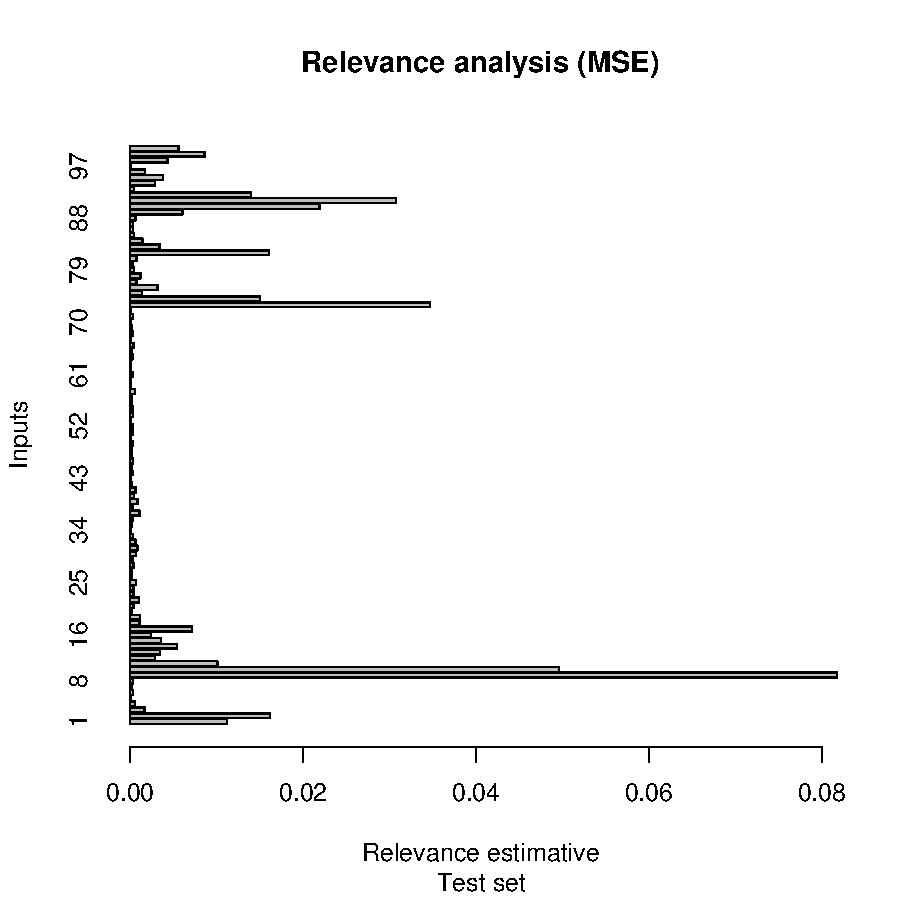
\includegraphics[scale=0.98]{ringer-mlp/test-mse-relevance}
\end{center}
\caption{Os valores de relevância para os conjunto de teste, para as 100
variáveis do anelador e considerando-se o classificador neural em estudo.}
\label{fig:ringer-mse-relevance}
\end{figure}

\begin{figure}
\begin{center}
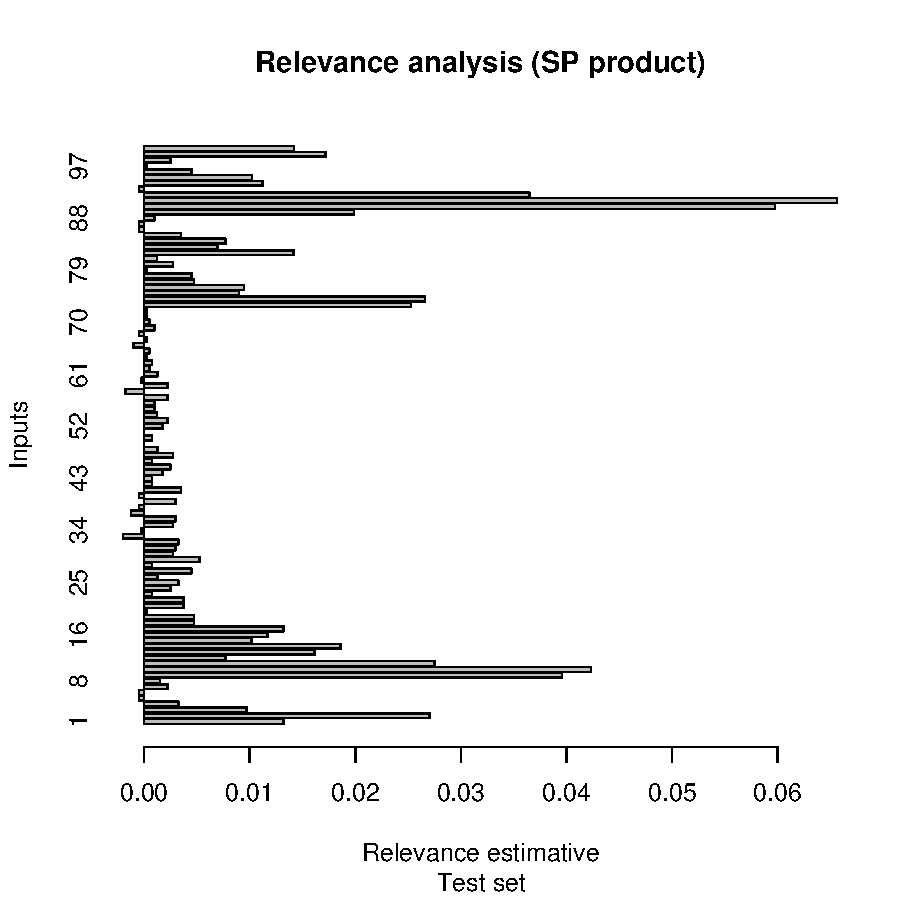
\includegraphics[scale=0.98]{ringer-mlp/test-sp-relevance}
\end{center}
\caption{Os valores de relevância de discriminação para os conjunto de teste,
para as 100 variáveis do anelador e considerando-se o classificador neural em
estudo.}
\label{fig:ringer-sp-relevance}
\end{figure}

\begin{table}
\begin{center}
\begin{tabular}{|l|r|r|r|} \hline
\textbf{Camada} & \textbf{Número de anéis} & \textbf{Primeiro} &
\textbf{Último} \\ \hline
Pré-irradiador & 8 & 1 & 8 \\
1\eira e.m. & 64 & 9 & 72 \\
2\eira e.m. & 8 & 73 & 80 \\
3\eira e.m. & 8 & 81 & 88 \\
1\eira hadrônica & 4 & 89 & 92 \\
2\eira hadrônica & 4 & 93 & 96 \\
3\eira hadrônica & 4 & 97 & 100 \\ \hline
\end{tabular}
\end{center}
\caption{Posicionamento relativo dos anéis produzidos pelo anelador no vetor
de entrada ao sistema de deteção neural.}
\label{tab:ringer-position}
\end{table}

\subsection{Compressão baseada na relevância}

A informação de relevância estudada até aqui pode ser aproveitada para que
aplique-se sobre as entradas do discriminador neural, uma poda baseada na
capacidade discriminante de uma variável. Esta poda pode ser feita
automaticamente \cite{andre-enfpc2000} em muitos casos, ou manualmente se
existirem restrições no processo de poda.

De fato, a técnica de normalização seqüêncial dos anéis que é proposta nesta
seção assume a disponbilidade da energia total camada a camada para o cálculo
do fator de normalização para cada anel. Ademais, para calcular o fator de
normalização para o anel $N+1$ em uma mesma camada, necessita-se do valor de
energia do anel $N$. Portanto, se deseja-se manter o anel $N+1$ de uma camada,
é necessário que se mantenha o anel $N$, ao menos para o cálculo do fator de
normalização. De fato, como veremos mais a frente, esta última sugestão seria
uma prática que recompensaria em pouco, visto que a maior parte do tempo de
processamento não está na discriminação neural e sim na aquisição dos
dados. Por outro lado, seria possível considerar que uma poda sempre seria
positiva no que tange a complexidade do discriminador neural que segue o
sistema de anelamento. Ao retirar uma variável da entrada, ao menos 8 conexões
sinápticas do detetor final seriam removidas simultaneamente, levando-se em
consideração a configuração exemplificada anteriormente. 

Observando-se mais uma vez o gráfico da Figura~\ref{fig:ringer-sp-relevance},
podemos concluir que o grau de importância dos anéis diminui, num geral, do
pico de deposição energética ($N = 0$) para as bordas da RoI. Desta forma o
problema da otimização deste sistema, numa primeira aproximação, poderia se
resumir à poda de elementos da periferia, de acordo com a relevância de
discriminação observada naquele gráfico.

Outra técnica que empregaremos será a combinação de camadas menos relevantes,
reduzindo o número de entradas do processador neural, sem que se perca,
necessariamente, a informação de energia presente nos anéis removidos. Uma
outra forma de manter a informação de energia, mas compactando ainda mais a
entrada seria a utilização de anéis cuja a largura dependesse da relevância
dos dados naquela região. Este estudo, reservaremos a um outro projeto. Tendo
em vista a discussão nos parâgrafos anteriores, propõe-se a seguinte variante
do processo de anelamento, baseando-se na relevância de discriminação da
Figura~\ref{fig:ringer-sp-relevance}

\begin{enumerate}
\item \textbf{Pré-irradiador}: utilizar apenas 4 ao invés de 8 anéis, com a
mesma granularidade anterior;
\item \textbf{1\eira\ camada e.m.}: utilizar apenas 12 dos 64 anéis iniciais, com a
mesma granularidade anterior;
\item \textbf{2\eira\ camada e.m.}: utilizar apenas 6 dos 8 anéis iniciais, com a
mesma granularidade anterior;
\item \textbf{3\eira\ camada e.m.}: utilizar apenas 4 dos 8 anéis iniciais, com a
mesma granularidade anterior;
\item \textbf{1\eira\ camada hadrônica}: manter a configuração atual;
\item \textbf{2\eira\ e 3\eira\ camadas hadrônica}: aglutinar em uma mesma
``camada'' virtual, mantendo a granularidade anterior.
\end{enumerate} 

Um novo total de 34 anéis é calculado da massa de dados originais. Em seguida,
cinco testes mantendo a mesma parametrização do sistema anterior foram
conduzidos. A R.O.C. do melhor destes testes, junto àquelas dos testes
anteriores, pode ser vista na Figura~\ref{fig:relev-cut1-roc}. A figura mostra
que o sistema podado se comporta tão bem quanto o sistema original com o 100
anéis, o superando em alguns pontos. Este novo sistema possui apenas a
terceira parte do número de anéis do sistema anterior, mas tem um desempenho
marginalmente melhor. O discriminador neural tem $66 \times 8 = 528$ menos
conexões sinápticas, somando um total de $289$ sinapses. O máximo do produto
SP ($1,82$) é atingido para uma eficiência na deteção de elétrons de $96,6$\%
contra um falso-alarme em jatos de apenas $2,94$\% (735~Hz).

\begin{figure}
\begin{center}
\includegraphics[scale=0.98]{ringer-mlp/relevance-cut1-roc}
\end{center}
\caption{R.O.C. comparativa entre os sistemas de deteção de elétrons e jatos
analisados até agora e o novo sistema de deteção gerado à partir da poda dos
canais de entrada baseada na relevância.}
\label{fig:relev-cut1-roc}
\end{figure}

A Figura~\ref{fig:relevance-cut1-sp-relevance} contém os valores de relevância
de discriminação para o detetor em questão. A
Tabela~\ref{tab:ringer-position-relevance-cut1} contém a posição relativa de
cada anel dentro do conjunto. A relação de relevância entre os anéis mudou
para este sistema. Anteriormente, os anéis da parte hadrônica eram os mais
relevantes ao processo discriminativo, a passo que neste novo sistema, os
anéis da primeira camada e.m. se mostram mais importantes. Dentro desta
camada, a ordem de importância não decresce com a distância ao pico de
deposição energética, apresentando um padrão menos estruturado.

A primeira camada e.m., como mostra a Figura~\ref{fig:lar-detail} no
Capítulo~\ref{chap:atlas}, é uma camada mais fina, originalmente concebida
para a deteção de jatos de partículas \cite{lar-tdr}. Estes objetos podem ser
também caracterizados analisando-se os padrões de deposição nesta camada:
múltiplas células sensibilizadas dentro de uma mesma RoI aumentam a
probabilidade do objeto em análise não ser um elétron. De fato, a variável
$\eratio$ do T2Calo assume exatamente este papel, como explicado no início do
Capítulo~\ref{chap:baseline}. Por esta razão, é bastante intuitivo que os
dados na primeira camada e.m. apresentem um padrão de relevância distinto aos
das demais camadas. De fato, o mesmo fenômeno pode também ser observado na
Figura`\ref{fig:ringer-sp-relevance}, embora neste contexto a informação
esteja menos evidente dado o contraste entre valores de relevância baixos para
os outros aneís. Para as outras camadas, a relevância parece ser maior para o
segundo anel que para o primeiro, caindo à medida que se afasta do centro.

\begin{figure}
\begin{center}
\includegraphics[scale=0.98]{ringer-mlp/relevance-cut1-sp-relevance-test}
\end{center}
\caption{Relevâncias de discriminação para o detetor neural baseado em 34 (dos
100) anéis resultantes da poda por relevância.}
\label{fig:relevance-cut1-sp-relevance}
\end{figure}

\begin{table}
\begin{center}
\begin{tabular}{|l|r|r|r|} \hline
\textbf{Camada} & \textbf{Número de anéis} & \textbf{Primeiro} &
\textbf{Último} \\ \hline
Pré-irradiador & 4 & 1 & 4 \\
1\eira e.m. & 12 & 5 & 16 \\
2\eira e.m. & 6 & 17 & 22 \\
3\eira e.m. & 4 & 23 & 26 \\
1\eira hadrônica & 4 & 27 & 30 \\
2\eira e 3\eira\ hadrônicas & 4 & 31 & 34 \\ \hline
\end{tabular}
\end{center}
\caption{Posicionamento relativo dos anéis produzidos pelo sistema de
anelamento podado para ter apenas 34 (dos 100) anéis.}
\label{tab:ringer-position-relevance-cut1}
\end{table}

%Levando-se em consideração a largura dos anéis e uma RoI que tem por base um
%tamanho de $\Delta_\eta\times\Delta_\phi = 0,4 \times 0,4$. Este novo sistema
%utiliza uma área cerca 

Uma vez que a eficiência deste novo sistema de deteção não foi afetada pela
poda, propõe-se uma segunda poda com a seguinte configuração:

\begin{enumerate}
\item \textbf{Pré-irradiador}: não se utilizará os dados desta camada;
\item \textbf{1\eira\ camada e.m.}: utilizar apenas 6 dos 64 anéis iniciais,
com a mesma granularidade anterior;
\item \textbf{2\eira\ camada e.m.}: utilizar apenas 4 dos 8 anéis iniciais,
com a mesma granularidade anterior;
\item \textbf{3\eira\ camada e.m.}: não se utilizará os dados desta camada;
\item \textbf{1\eira\ camada hadrônica, 2\eira\ e 3\eira\ camadas hadrônica}: aglutinar em uma mesma ``camada'' virtual, mantendo a granularidade anterior.
\end{enumerate} 

Um total de 14 anéis restam nesta nova configuração. Mantém-se os parâmetros
de treinamento e o número de neurônios na camada escondida do detetor neural
inicial. A Figura~\ref{fig:relev-cut2-roc} mostra a curva R.O.C. de um dos 5
testes realizados, junto à curva R.O.C. dos outros detetores. Mais uma vez o
sistema não apresenta perda no desempenho comparado ao sistema original com
100 anéis. O ponto de máximo do produto SP ocorre quando a eficiência na
deteção de elétrons é de $96,89$\% contra um falso-alarme de $2,72$\%
(680~Hz).

\begin{figure}
\begin{center}
\includegraphics[scale=0.98]{ringer-mlp/relevance-cut2-roc}
\end{center}
\caption{R.O.C. comparativa entre os sistemas de deteção de elétrons e jatos
analisados até agora e o novo sistema de deteção baseado na poda da
relevância, com apenas 14 (dos 100) anéis.}
\label{fig:relev-cut2-roc}
\end{figure}

A Figura~\ref{fig:relevance-cut2-sp-relevance} contém os valores de relevância
de discriminação para a segunda poda baseada no critério da relevância de
discriminação. A Tabela~\ref{tab:ringer-position-relevance-cut2} mostra a
relação entre os números naquele gráfico. Neste novo sistema, a parte
hadrônica re-adquire a importância do sistema baseado nos 100 anéis,
recuperando, possivelmente, a falta de dados para a terceira camada e.m., que
foi suprimida nesta avaliação.

\begin{figure}
\begin{center}
\includegraphics[scale=0.98]{ringer-mlp/relevance-cut2-sp-relevance-test}
\end{center}
\caption{Relevâncias de discriminação para o detetor neural baseado em 14 (dos
100) anéis resultantes da poda por relevância.}
\label{fig:relevance-cut2-sp-relevance}
\end{figure}

\begin{table}
\begin{center}
\begin{tabular}{|l|r|r|r|} \hline
\textbf{Camada} & \textbf{Número de anéis} & \textbf{Primeiro} &
\textbf{Último} \\ \hline
1\eira e.m. & 6 & 1 & 6 \\
2\eira e.m. & 4 & 7 & 10 \\
1\eira\, 2\eira e 3\eira\ hadrônicas & 4 & 11 & 14 \\ \hline
\end{tabular}
\end{center}
\caption{Posicionamento relativo dos anéis produzidos pelo sistema de
anelamento podado usando a análise de relevância discriminante, para ter
apenas 14 (dos 100) anéis.}
\label{tab:ringer-position-relevance-cut2}
\end{table}

\subsection{Desempenho do sistema de discriminação}
\label{sec:performance}

O algoritmo apresentado nesta seção deve respeitar as normas de operação do
Segundo Nível de Filtragem do experimento. Neste nível de filtragem, espera-se
que o tempo médio de processamento para cada evento, incluindo acesso aos
dados no sistema de leitura, seja de 10 milissegundos. No entanto, espera-se
que o sistema opere rejeitando eventos ordinários o mais rápido possível, de
tal forma que, estatisticamente, a maior parte do tempo despendida nos
processadores do LVL2 seja dedicada à eventos interessantes.

Levando-se em consideração que o tempo de acesso aos dados no sistema de
leitura está na ordem de 1~ms, como descrito no Capítulo~\ref{chap:trigger},
deseja-se minimizar o tempo de processamento despendido no algoritmo. Desta
forma, medidas de desempenho são normalmente executadas nos candidatos à
algoritmos ao sistema de filtragem, de modo a determinar seu tempo de execução
e possíveis pontos a serem otimizados.

Nossa referência, o algoritmo do T2Calo, foi completamente descrita na
Seção~\ref{sec:lvl2-detect-electron}. Neste algoritmo, inicia-se o
processamento detetando-se o pico na segunda camada e.m., seguindo-se do
cálculo da variável $\rcore$. A variável $\eratio$ é calculada em seguida,
utilizando-se dos dados da primeira camada e.m.. De posse dos valores parciais
de energia nestas duas camadas, os dados do pré-irradiador e da terceira
camada e.m. são utilizados para definir o valor da variável $\etem$. Na última
parte do processamento define-se o valor da variável $\ethad$, acessando-se os
dados da parte hadrônica. A Tabela~\ref{tab:t2calo-performance} contém as mais
recentes medidas realizadas na avaliação do desempenho do T2Calo
\cite{denis-presentation}. Os valores nesta tabela representam o tempo médio
de processamento, em milissegundos, para cada uma das fases. Estes tempos
também desconsideram a execução do algoritmo de hipótese EGammaHypo. Assume-se
no entanto, que seja desprezível, dado sua simplicidade.

\begin{table}
\begin{center}
\begin{tabular}{|l|r|r|r|} \hline
\textbf{Fase} & \textbf{Calib. e Localização} & 
\textbf{Algoritmo} & \textbf{Tot. parcial}\\ \hline
$\rcore$ & 0,45 & 0,49 & 0,94 \\ 
$\eratio$ & 0,48 & 0,57 & 1,05 \\ 
$\etem$ & 0,56 & 0,17 & 0,73 \\ 
$\ethad$ & 0,59 & 0,33 & 0,92 \\ \hline
\textbf{Total} & \textbf{2,08} & \textbf{1,56} & \textbf{3,64} \\ \hline
\end{tabular}
\end{center}
\caption{Tempo de processamento médio das diversas fases do algoritmo T2Calo
em uma máquina com processadores Intel Xeon de 2,4 GHz e 1~Gb de memória RAM.}
\label{tab:t2calo-performance}
\end{table}

Tomando-se por base que um sistema baseado no anelamento e deteção neural terá
que acessar os mesmos dados que o T2Calo acessa, a primeira parte do tempo
torna-se uma constante para os propósitos deste trabalho. A segunda parte, no
entanto, é completamente dependente do algoritmo e devemos compará-la ao tempo
de execução do \eng{NeuralRinger}.

A complexidade de execução do método baseado no anelador e deteção neural é
variável de acordo com dois parâmetros principais:

\begin{enumerate}
\item Com o número de aneís que se deseja extrair: neste caso, quanto mais
anéis deseja-se extrair dos dados, maior o tempo de execução que será
necessário para cumprir o processo de anelamento. Ademais, com o aumento do
número de anéis aumenta-se igualmente o tamanho da entrada do discriminador
neural e, portanto, o número de operações aritméticas para esta última fase do
processamento;
\item O número de neurônios escondidos na rede neural também influenciará o
tempo de execução do discriminador.
\end{enumerate}

Para determinar a viabilidade em termos desempenho, para algoritmo proposto
por este trabalho, executou-se a aplicação \texttt{ringer-run} em um conjunto
de máquinas de refência ao experimento ATLAS. A
Tabela~\ref{tab:machine-comparison} resume as características destas
máquinas. A primeira das máquinas listadas está sendo utilizada em uma
avaliação de arquiteturas para o sistema de filtragem e aquisição de dados do
ATLAS, conhecido como \textit{pré-série}, (do inglês, \eng{preseries})
\cite{gokhan-chep06}. Esta é a máquina de referência máxima para estudos de
desempenho no ATLAS. A segunda máquina de teste é um modelo com dois núcleos
(do inglês, \eng{dual-core}). A arquitetura desta máquina está sendo
considerada como opção às máquinas atualmente empregadas nas pré-séries, sendo
este modelo de processador o mais recente disponibilizado pelo fabricante. A
terceira e última máquina faz parte de um conjunto de máquinas dedicada a
estudos do sistema de filtragem. Embora possua uma arquitetura mais antiga,
ainda é usada como referência em muitos trabalhos, sendo este o caso das
medidas do T2Calo apresentadas acima.

\begin{table}
\begin{center}
\begin{tabular}{|l|l|r|r|} \hline
Processador & \eng{Clock} & \eng{Cache} de L2 & Memória RAM \\ \hline
AMD Opteron (250) & 2,4~GHz & 1~Mb & 4~Gb \\
AMD Opteron (275) & 2,2~GHz & 1~Mb & 4~Gb \\
Intel Xeon & 2,4~GHz & 512~kb & 1~Gb \\ \hline
\end{tabular}
\end{center}
\caption{Configurações das máquinas utilizadas para o teste de desempenho do
\eng{NeuralRinger}.}
\label{tab:machine-comparison}
\end{table}

Estas máquinas contém uma instalação completamente funcional do sistema
operacional atualmente empregado no CERN, o SLC3 \cite{cern-linx}. Embora
alguns dos processadores possam operar em 64-bits (assim como o
\eng{NeuralRinger}), estas máquinas são operadas em modo de compatibilidade
para 32-bits, já que grande parte do \eng{software} do ATLAS ainda não opera
corretamente nesta plataforma.

Um conjunto idêntico, composto de três diferentes testes foram executados em
cada uma das máquinas, utilizando todos os dados disponíveis (cerca de 22.600
elétrons e 7500 jatos) para este estudo. Para estes testes utilizou-se o
programa \texttt{ringer-run}, que executa as fases de anelamento e
discriminação em seqüência, como aconteceria num sistema \eng{online}.  Os
testes realizados em uma mesma máquina diferem entre si somente pela
configuração da anelamento e da rede neural que discriminará os dados após a
extração dos anéis. As combinações utilizadas equivalem àquelas dos testes
mostrados anteriormente neste capítulo, para o sistema com 100 anéis, o
sistema podado com 34 anéis e o último, utilizando apenas os 14 mais
relevantes anéis. Durante os testes, observou-se a quantidade de memória RAM
disponível na máquina de tal forma que o carregamento dos dados não ativasse o
mecanismo de troca de disco (do inglês, \eng{swap}), já que isso faria com que
a aplicação tivesse um desempenho abaixo do esperado para o experimento.

As Figuras~\ref{fig:timings-histo-full}, \ref{fig:timings-histo-cut1} e
\ref{fig:timings-histo-cut2} contém os resultados dos 3 testes com 100, 34 e
14 anéis respectivamente nas três arquitecturas. Das três arquiteturas
escolhidas, a máquina da pré-série parece ser a mais rápida, apresentando um
tempo de processamento de apenas $445$ microssegundos para o mais complexo dos
testes, utilizando 100 anéis. Em seguida, o sistema baseado no processor
Opteron-275, cerca de 8\% mais lento para o mesmo teste. A máquina de testes
do sistema de filtragem é a mais lenta de todas as plataformas, apresentando
um tempo médio de processamento de $542$ microssegundos para cada RoI. O
desvio padrão está na faixa dos 10\% indicando uniformidade nos resultados.

\begin{figure}
\begin{center}
\includegraphics[scale=0.98]{ringer-mlp/compare-test-full-rings}
\end{center}
\caption{Tempos totais de executação do \eng{NeuralRinger} em três plataformas
distintas, utilizando 100 anéis.}
\label{fig:timings-histo-full}
\end{figure}

\begin{figure}
\begin{center}
\includegraphics[scale=0.98]{ringer-mlp/compare-test-cut1-rings}
\end{center}
\caption{Tempos totais de executação do \eng{NeuralRinger} em três plataformas
distintas, utilizando 34 anéis.}
\label{fig:timings-histo-cut1}
\end{figure}

\begin{figure}
\begin{center}
\includegraphics[scale=0.98]{ringer-mlp/compare-test-cut2-rings}
\end{center}
\caption{Tempos totais de executação do \eng{NeuralRinger} em três plataformas
distintas, utilizando apenas 14 anéis.}
\label{fig:timings-histo-cut2}
\end{figure}

Nos testes seguintes, a relação entre o desempenho das máquinas se
mantém. Para o teste com 34 anéis o tempo de processamento médio na máquina
mais rápida é de $215$ microssegundos, tendo caído aproximadamente a metade do
valor para os 100 anéis. Para o teste com apenas 14 dos 100 anéis originais, o
tempo médio de processamento é de apenas $125$ microssegundos para a máquina
mais veloz, representando quase um-quarto do tempo de processamento para o
sistema de anelamento completo.

Ao compararmos o mais complexo dos exercícios com o tempo de referência do
T2Calo (1,56~ms) para a mesma plataforma, observa-se que o sistema proposto
executa em apenas um-terço do tempo requerido para o T2Calo nesta
arquitetura. Esta análise não leva em conta o acesso aos dados e sua
calibração e localização dentro das bibliotecas de infrastrutura do LVL2. Pela
Tabela~\ref{tab:t2calo-performance}, nota-se que cerca de 57\% do tempo total
do processamento de uma RoI, isto é, aproximadamente 2,1~ms é devido a esta
parte dos dados. Desta forma conclui-se que o sistema proposto pelo anelador
está dentro das especificações de desempenho para o sistema de filtragem do
ATLAS.

A Figura~\ref{fig:p1-full-histos} mostra os histogramas individuais para cada
uma das fases de processamento, para o teste usando 100 anéis rodando na
máquina mais rápida (Opteron/250, 2,4~GHz). Desta figura conclui-se que, no
caso de tempos de processamento menores se tornarem imperativos, uma
implementação dedicada do processo de anelamento (originalmente implementado
na biblioteca \texttt{rbuild}) poderá ser realizada de forma que o tempo total
de deste algoritmo seja otimizado. Junto à discriminação neural as duas fases
representam mais de 90\% do tempo de processamento total. Otimizações na fase
de procura do pico de deposição energética na segunda camada e.m. ou na fase
de normalização dos anéis teriam quase ou nenhum impacto considerando-se a
arquitetura atual do \eng{NeuralRinger}.

\begin{figure}
\begin{center}
\includegraphics[scale=0.98]{ringer-mlp/full-histos-opteron-250}
\end{center}
\caption{Tempos individuais para cada fase de execução do \eng{NeuralRinger},
levando-se em consideração a extração e discriminação baseada em 100 anéis. O
teste foi executado na plataforma Opteron/250 (pré-serie).}
\label{fig:p1-full-histos}
\end{figure}

\subsection{Migração para o sistema de filtragem do ATLAS}

O projeto do \eng{NeuralRinger} evoluiu ao longo de 2 anos de desenvolvimento
de forma que se tornasse facilmente integrável ao ambiente de funcionamento
\eng{online}, que é baseado no \eng{framework} Athena
\cite{athena:home-page, athena:devel-guide}. Neste âmbito, o projeto de um
detetor neural baseado na técnica de anelamento deve seguir os seguintes
passos:

\begin{enumerate}
\item Encontrar os dados que serão utilizados para treino e teste do
discriminador neural. Rodar o programa \texttt{athena}, de forma a extrair
dados no formato nativo do \eng{NeuralRinger};
\item Projetar e treinar o sistema de anelamento e detetor neural no ambiente
do \eng{NeuralRinger};
\item Aplicar as configurações de anelamento e deteção neural no sistema
\eng{online}.
\end{enumerate}

Desta forma, é possível desacoplar o desenvolvimento de detetores ao uso do
ambiente Athena, o que é uma vantagem considerável: diminui-se o tempo de
desenvolvimento e permite-se que o usuário foque sua atenção ao problema da
classificação sem se importar com os detalhes, muitas vezes complexos, deste
ambiente. Os resultados da aplicação de um detetor específico, dentro e fora
do ambiente Athena devem ser idênticos.

\subsubsection{\eng{NeuralRinger} e o Athena}

Para que seja facilmente integrável dentro do ambiente Athena, o
\eng{NeuralRinger} segue a filosofia de funcionamento deste ambiente. Cada uma
das fases de processamento, i.e., a criação dos anéis de energia e a
classificação neural estão codificadas em bibliotecas individualizadas e podem
ser utilizadas tanto conjunta quanto separadamente. No ambiente
\eng{online}, a extração de características e deteção são normalmente
separadas de forma que possam ser desenvolvidas independentemente.

O processamento do evento dentro do sistema filtragem ocorre de forma
seqüencial, como explicado na Seção~\ref{sec:hlt}. Para cada objeto ou RoI
destacado pelo nível de filtragem antecedente, o componente do HLT conhecido
como \eng{Steering} (que poderia ser traduzido, neste contexto, como
Coordenador ou Agendador) irá definir o algoritmo que será chamado para
tratá-lo. O algoritmo poderá realizar um conjunto de operações no objeto em
questão, aumentando a quantidade de informações disponíveis para análise deste
ítem ou interrompendo o processamento.

Desta forma, é possível definir duas classes de algoritmos:

\begin{itemize}
\item \textbf{Extração}: Algoritmos que apenas adicionam informação a um
objeto no evento, através da extração de características nos dados do detetor;
\item \textbf{Hipótese}: Algoritmos que interrompem o processamento de um
objeto por o considerarem como física ordinária que não deve ser registrada em
mídia permanente.
\end{itemize}

Sendo, o processo de hipótese, separado do processo de extração, é possível
desenvolver sistemas de decisão mais e mais complexos conforme se avance
dentro da análise do evento. A Figura~\ref{fig:simple-menu} exemplifica este
cenário para uma configuração fictícia para o \eng{Steering}. Este é um
exemplo que pode ser reproduzido no LVL2: um objeto tipo e.m. é encontrado no
resultado do LVL1 passado ao \eng{Steering}. Este objeto causa o agendamento
de um algoritmo que possa tratá-lo. A primeira fase do processamento é a
extração de características do objeto. Neste exemplo, a primeira extração de
característica considerada é a extração dos anéis. O passo seguinte a extração
é a hipótese. Se o objeto atender às características de um elétron, o
\eng{Steering} irá agendar o passo seguinte. Caso, não, a hipótese de que o
objeto seja um objeto tipo e.m. é rejeitada e o processamento é parado,
causando a rejeição do evento pelo sistema de filtragem. Caso a hipótese seja
afirmativa, neste exemplo, tentar-se-á encontrar um traço relativo ao objeto
nos detetores de traço. Caso isto falhe, o objeto será rejeitado como indica a
figura. Se, finalmente, nenhuma das fases de processamento conseguir rejeitar
o objeto, ele será rotulado como um elétron, os valores extraídos das
características do objeto serão apendicionadas a este novo elemento e o evento
será aprovado.

\begin{figure}
\begin{center}
\includegraphics[scale=0.40]{simple-menu}
\end{center}
\caption{Exemplo de um cenário de seleção simples para o \eng{Steering}
operando no LVL2, baseado em uma RoI tipo E.M..}
\label{fig:simple-menu}
\end{figure}

Para atender à alta complexidade do experimento, muitas seqüências como a
descrita na Figura~\ref{fig:simple-menu} podem co-existir dentro do
\eng{Steering}. Cabe a este sistema de agendamento escolher apropriadamente
a seqüência de passos e combinações de objetos apropriadas para que se possa
analisar o evento adequadamente.

Para a integração do \eng{NeuralRinger} e observando-se a estrutura de
processamento \eng{online}, divide-se o anelamento e a decisão neural em dois
passos distintos, que podem ser executados independentemente. Para evitar a
dispersão de código, criou-se 3 pacotes assim denominados:

\begin{itemize}
\item \textbf{TrigRingerTools}: Este pacote contém as bibliotecas 
originais do \eng{NeuralRinger} e é usado como base funcional dos outros
pacotes;
\item \textbf{TrigCaloRinger}: Este pacote implementa um algoritmo de 
extração de características. As características neste caso são os valores
energéticos dos anéis;
\item \textbf{TrigMultiVarHypo}: Este pacote implementa um algoritmo de
hipótese baseada em redes neurais. Nele encontra-se a implementação do
algoritmo de hipótese baseada em redes neurais. 
\end{itemize}

Com esta configuração é possível manter o conjunto de bibliotecas do
\eng{NeuralRinger} coeso em um único pacote (\texttt{TrigRingerTools}) e
apenas implementar um conjunto de algoritmos que usam a funcionalidade de base
deste pacote. Os algoritmos de extração de características e hipótese são
configuráveis em todos os aspectos da sua versão desacoplada e podem escrever
em disco os resultados parciais de suas operações para verificação externa ao
Athena.

Para determinar o correto funcionamento deste sistema, é necessário testar,
baseado na entrada, a saída de cada passo, para um conjunto de eventos. Para
tal, utilizou-se uma base de dados com eventos simulados tipo $Z \rightarrow
e^- + e^-$ que estava disponível no formato adequado. Uma configuração de
anelamento utilizando 100 anéis como descritos anteriormente e uma rede neural
com 100 entradas, 8 neurônios escondidos e um neurónio na camada de
saída. Cerca de 850 RoI's foram selecionadas pela simulação do LVL1 indicando
objetos a serem averiguados no LVL2. Roda-se o sistema Athena, configurado
para utilizar os algoritmos de anelamento e deteção neural extraindo-se 3
tipos de dados:

\begin{enumerate}
\item O valores de energia e posicionamento das células utilizadas para o
cálculo dos anéis, num formato compatível com o padrão do \eng{NeuralRinger}; 
\item Uma base de dados de anéis já processados e normalizados, em formato
XML;
\item Uma base de dados com as saídas do processamento neural, também no
formato XML.
\end{enumerate}

Com base na versão desacoplada do \eng{NeuralRinger}, executa-se os mesmos
processos:

\begin{enumerate}
\item Basedo nos valores originais das células provida pelo Athena, calcula-se
os anéis; 
\item Baseado na saída dos anéis provida pelo Athena, calcula-se a saída da
rede neural.
\end{enumerate}

A Figura~\ref{fig:athena-vs-nr} mostra as diferenças, RoI a RoI, nos cenários
1 e 2 descritos anteriormente. Como é possível observar no primeiro histograma
desta figura, os resultados são idênticos com uma precisão melhor que $1
\times 10^{-7}$ no caso do Teste~1. Este erro existe pois os valores relativos
às energias das células, escritos em disco para a análise pelo
\eng{NeuralRinger}, são truncados na décima casa decimal.

\begin{figure}
\begin{center}
\includegraphics[scale=0.98]{athena-vs-nr-error}
\end{center}
\caption{Erros entre os processos de extração de características e hipótese
neural entre o Athena e o \eng{NeuralRinger} rodando em modo desacoplado.}
\label{fig:athena-vs-nr}
\end{figure}

Para o Teste~2, no histograma na parte inferior da
Figura~\ref{fig:athena-vs-nr}, o resultados são idênticos para uma precisão
melhor que $2 \times 10^{-6}$. Este erro existe pois os valores relativos às
energias dos anéis, escritos em disco para a análise pelo \eng{NeuralRinger},
são truncados à partir da sexta casa decimal.

Para completar a análise, roda-se o processo completo de extração e
classificação neural, baseando-se nos valores das células, comparando a saída
deste procecedimento à saída provida pelo sistema neural acoplado ao ambiente
Athena. A Figura~\ref{fig:athena-vs-nr-full} mostra um gráfico de dispersão
das saídas dos dois sistemas para as configurações de anelamento e rede neural
descritas anteriormente. Neste caso, onde não há escrita em disco entre os
dois passos do processamento, o erro observado é literalmente zero entre os
dois sistemas. Estes resultados, portanto, indicam que a precisão de escrita é
suficiente para a reprodução desacoplada e que o sistema migrado funciona
adequadamente.
% Cabe-se notar que a rede neural utilizada para este teste não
%havia sido treinada para a deteção eficiente de dados com empilhamento, sendo
%esta a razão da distribuição tão homegênea da saída do detetor neural.

\begin{figure}
\begin{center}
\includegraphics[scale=0.98]{athena-vs-nr-error-full-chain}
\end{center}
\caption{Gráfico de dispersão entre a saída final do Athena e de uma versão do
\eng{NeuralRinger} rodando em modo desacoplado.}
\label{fig:athena-vs-nr-full}
\end{figure}

O segundo passo é a confirmação dos tempos de operação destacados na
Seção~\ref{sec:performance}. Neste caso deseja-se averiguar se a migração não
acarretou algum impacto ao desempenho do sistema. Por outro lado, obtém-se com
este estudo um conjunto de valores comparativos mais justos a outros
métodos. Por questões de praticidade ligadas à disponibilidade dos dados e
quantidade de memória disponível, escolhe-se a máquina baseada no processador
AMD Opteron $275$ utilizada anteriormente, para realizar-se os testes.

\paragraph{Serviço de Temporização do Athena:} O serviço de temporização do
Athena (no pacote \eng{TrigTimeSvc}) utiliza a função \texttt{gettimeofday}
\cite{web:gcc-libc} para executar a operação de medida de tempo entre dois
pontos quaisquer dentro do código. A utilização de um relógio em tempo-real é
benéfica quando deseja medir tempos de processamento com uma precisão menor
que 10~milissegundos (fornecida pela função \texttt{clock}). 

Um dos inconvenientes da função \texttt{gettimeofday} é que o valor obtido em
uma chamada é uma medida absoluta do tempo. Como um processo unix está sujeito
à interrompimentos de sua execução, o tempo parado também será contado
eventualmente. Ademais, máquinas modernas possuem normalmente mais de um
processador. É portanto provável que processos que estejam parados, neste
contexto, sejam mais rapidamente agendados. Desta forma, o tempo final
observado será uma mistura de tempos de execução reais, somados aos tempos de
parada e re-agendamento. Estes tempos não são normalmente significativos para
longos processos, mas pode facilmente afetar a percepção de processos mais
curtos. Para evitar que estes tipos de evento ocorram com freqüência durante
a medida de tempo, ajustou-se a prioridade de execução do processo Athena de
forma a minimizar o tempo que o processo estaria parado ou em transição de
processador.

A Figura~\ref{fig:timings-athena} mostra 7 histogramas correspondentes às
diversas fases do processamento do \eng{NeuralRinger} integrado ao ambiente
Athena. Na parte superior da figura, observa-se o tempo de acesso aos
dados. Este tempo de acesso é partilhado por todos os algoritmos de
calorimetria, e apresenta neste caso uma média de 2,2~milissegundos por
RoI. No ambiente Athena, este valor inclui o tempo de formatação dos dados no
padrão dos detetores do ATLAS. Os quatro histogramas que seguem representam
histogramas equivalentes aos da Figura~\ref{fig:p1-full-histos}, onde é
possível observar os tempos individuais de cada uma das fases do processo de
extração de características e classificação neural. Os dois histogramas no
final da figura mostram os tempos de processamento totais, por algoritmo.

\begin{figure}
\begin{center}
\includegraphics[scale=0.98]{timings-pcuwtr1}
\end{center}
\caption{Tempos de execução do \eng{NeuralRinger} funcionando integrado no
ambiente Athena.}
\label{fig:timings-athena}
\end{figure}

Removendo-se a contribuição do tempo de acesso aos dados, o processo de
extração leva em média $2720-2194=526$ microssegundos. O tempo médio de
classificação baseado em uma rede neural leva $259$ microssegundos. Desta
forma, o tempo total, comparável àquele da
Figura~\ref{fig:timings-histo-full}, é de $526+259=785$ microssegundos. Este
valor representa um acréscimo de cerca de 56\% do tempo total calculado
anteriormente. Uma parte do tempo adicional é gasto na criação de estruturas
de dados que sejam repassáveis entre os algoritmos, passo necessário no
ambiente Athena e que foi suprimido na execução desacoplada. Uma outra parte
advém da utilização da infrastrutura de acesso à dados e reportagem de erros
disponível no ambiente Athena, que é mais lenta que no ambiente desacoplado.

O tempo total de processamento do algoritmo integrado é de cerca de
3,2~milissegundos. Comparando-se os tempos relativos de processamento para
diversas configurações de anéis e detetores neurais das
Figuras~\ref{fig:timings-histo-full}, \ref{fig:timings-histo-cut1} e
\ref{fig:timings-histo-cut2} observa-se uma relação aproximadamente constante
de cerca de 10 a 15\% de diferença entre as plataformas AMD Opteron-275 e
Intel Xeon, dependendo do número de aneís utilizados. Escalando o valor de
tempo observado considerando-se a diferença máxima de 15\%, chega-se a um
valor de $\approx 3,8$ milissegundos. Este valor é comparável ao tempo total
na Tabela~\ref{tab:t2calo-performance}, de $3,64$ milissegundos. Portanto, com
este exercício, demonstra-se a viabilidade deste sistema de deteção para que
seja empregado \eng{online}.

A Figura~\ref{fig:timings-eta-dep} ilustra a dependência dos tempos parciais
de processamento com a localização da região de interesse, por $\eta$. A
Figura~\ref{fig:timings-phi-dep} mostra a relação com a variável
$\phi$. Naturalemente, o processo é tendencioso com relação à variável $\eta$,
devido às variações da granularidade e independente da localização em $\phi$.

\begin{figure}
\begin{center}
\includegraphics[scale=0.98]{timings-eta-dep}
\end{center}
\caption{Relação entre o posicionamento da RoI em $\eta$ e os tempos de
processamento do \eng{NeuralRinger} em diversas das fases da extração de
características no ambiente Athena.}
\label{fig:timings-eta-dep}
\end{figure}

\begin{figure}
\begin{center}
\includegraphics[scale=0.98]{timings-phi-dep}
\end{center}
\caption{Relação entre o posicionamento da RoI em $\phi$ e os tempos de
processamento do \eng{NeuralRinger} em diversas das fases da extração de
características no ambiente Athena.}
\label{fig:timings-phi-dep}
\end{figure}

\subsubsection{\eng{NeuralRinger} e o sistema de aquisição}

O último passo da integração é demonstração da viabilidade do sistema de
filtragem em um protótipo do sistema de aquisição, junto à outros algoritmos
de filtragem. Neste caso, inicialmente validamos o funcionamento do algoritmo
no contexto de uma configuração mais complexa baseada na aplicação AthenaMT
\cite{aa:tns-2004-2}, que simula, ainda \eng{offline}, o ambiente de aquisição
tal qual será encontrado pelos algoritmos do HLT \eng{online}. Este é um passo
simples, dado que re-utiliza-se o mesmo conjunto de bibliotecas usadas para o
ambiente Athena, sem necessitar que se recompilem-nas. A vantagem é que o
sistema já encontra-se depurado e a única verificação a ser feita é se a
utilização dos novos algoritmos não introduz erros para os demais.

Executou-se a aplicação AthenaMT incluindo uma configuração para a deteção de
objetos tipo e.m. (T2Calo e algoritmos de deteteção de traços) junto ao
sistema baseado no anelamento e deteção neural. Observou-se o consumo de
memória enquanto executava-se a aplicação para que se rastreie possíveis
vazamentos. Não foram observados problemas em nenhum aspecto.

O passo final é a configuração de uma bancada de testes para executar os
algoritmos dentro do ambiente do Sistema de Filtragem do ATLAS. Para tal
utilizou-se 7 máquinas conectadas via \eng{gigabit} ethernet e uma máquina
adicional para controlar o sistema remotamente.  A
Figura~\ref{fig:online-schema} esquematiza o sistema utilizado para o teste e
o mapeamento das diversas aplicações nas máquinas. Esta bancada é,
naturalmente, uma versão bastante reduzida do sistema que estará disponível no
experimento. Para emular as condições de funcionamento do ATLAS, carregam-se
dados de elétrons simulados nos nós nomeados \texttt{ROS-*} e
\texttt{L2SV-*}. Desta forma, para as L2PU's, as condições de operação são
idênticas ao do sistema final. A bancada consiste de 8 L2PU's, 8 Emuladores do
Sistema de Leitura do detetor (ROS) e 1 L2SV. Estes sistemas estão conectados
através de uma chave \eng{Gigabit ethernet} e conectados ao sistema
controlador através da rede do CERN.

\begin{figure}
\begin{center}
\includegraphics[scale=0.5]{online-schema}
\end{center}
\caption{Esquema de bancada de testes para a verificação do funcionamento do
NeuralRinger dentro do ambiente de aquisição de dados do ATLAS.}
\label{fig:online-schema}
\end{figure}

O sistema de filtragem e aquisição do ATLAS provê um conjunto de ferramentas
que podem ser utilizadas para monitorar a execução do sistema. A
Figura~\ref{fig:ringer-screenshot} mostra uma captura de tela na máquina
controladora, mostrando algumas destas ferramentas em atuação durante o
teste. A luz verde na maior das janelas indica que o sistema está operante e
nenhum erro foi detetado. O número de eventos processado, no total, pelas oito
unidades de processamento é de aproximadamente meio milhão. O valor está
marcado em vermelho na parte inferior esquerda da figura. A taxa de
funcionamento do sistema parece estável em cerca de 245~Hz, como indica o
gráfico na parte inferior direita da figura. Na parte superior direita, uma
janela do sistema de monitoração \eng{online} mostra um histograma, preenchido
durante a execução do sistema e atualizado durante a operação com o tempo de
processamento de um dos algoritmos de anelamento rodando na L2PU número 2. O
tempo de processamento médio deste algoritmo nesta L2PU é de cerca de
3,8~ms. Este tempo inclui o tempo de acesso aos dados através da rede
\eng{Gigabit ethernet} levando-se em conta a configuração da bancada.

\begin{figure}
\begin{center}
\includegraphics[scale=0.33]{ringer-online-3}
\end{center}
\caption{Captura de tela mostrando a operação do sistema de extração de
características baseado em anéis rodando dentro de uma banca de testes do
sistema de filtragem e aquisição do ATLAS.}
\label{fig:ringer-screenshot}
\end{figure}

\typeout{ *************** End of file neuralringer.tex *************** }
